%!TEX encoding = UTF-8 Unicode
\documentclass[a4paper]{compendium}

%\usepackage{xr} %to crossreference ???
\externaldocument{lectures} %to crossreference
\externaldocument{exercises} %to crossreference


\usepackage[swedish]{babel}
\addto\captionsswedish{%
  \renewcommand{\appendixname}{Appendix}%
}
%TODO: Glossary
%http://tex.stackexchange.com/questions/5821/creating-a-standalone-glossary/5837#5837

\setlength{\columnsep}{16mm}

\newcommand{\LibVersion}{0.1.0} % latest version of introlib at https://github.com/lunduniversity/introprog-scalalib
\newcommand{\LibJar}{\texttt{introprog-\LibVersion.jar}}
\newcommand{\JDKApiUrl}{\url{https://docs.oracle.com/javase/8/docs/api/}}


\title{
{\vspace{-3.0cm}\bf\sffamily\Huge\selectfont  Introduktion till programmering med Scala}
\\ \vspace{1em}%\hspace*{1.5cm}\inputgraphics[width=0.6\textwidth]{../img/gurka} \\
{\sffamily  Laborationer och projekt}\\\vspace{2cm}
%
\includegraphics[height=4cm]{../img/scala-logo.png}
%
\includegraphics[height=4cm]{../img/java-logo.png}
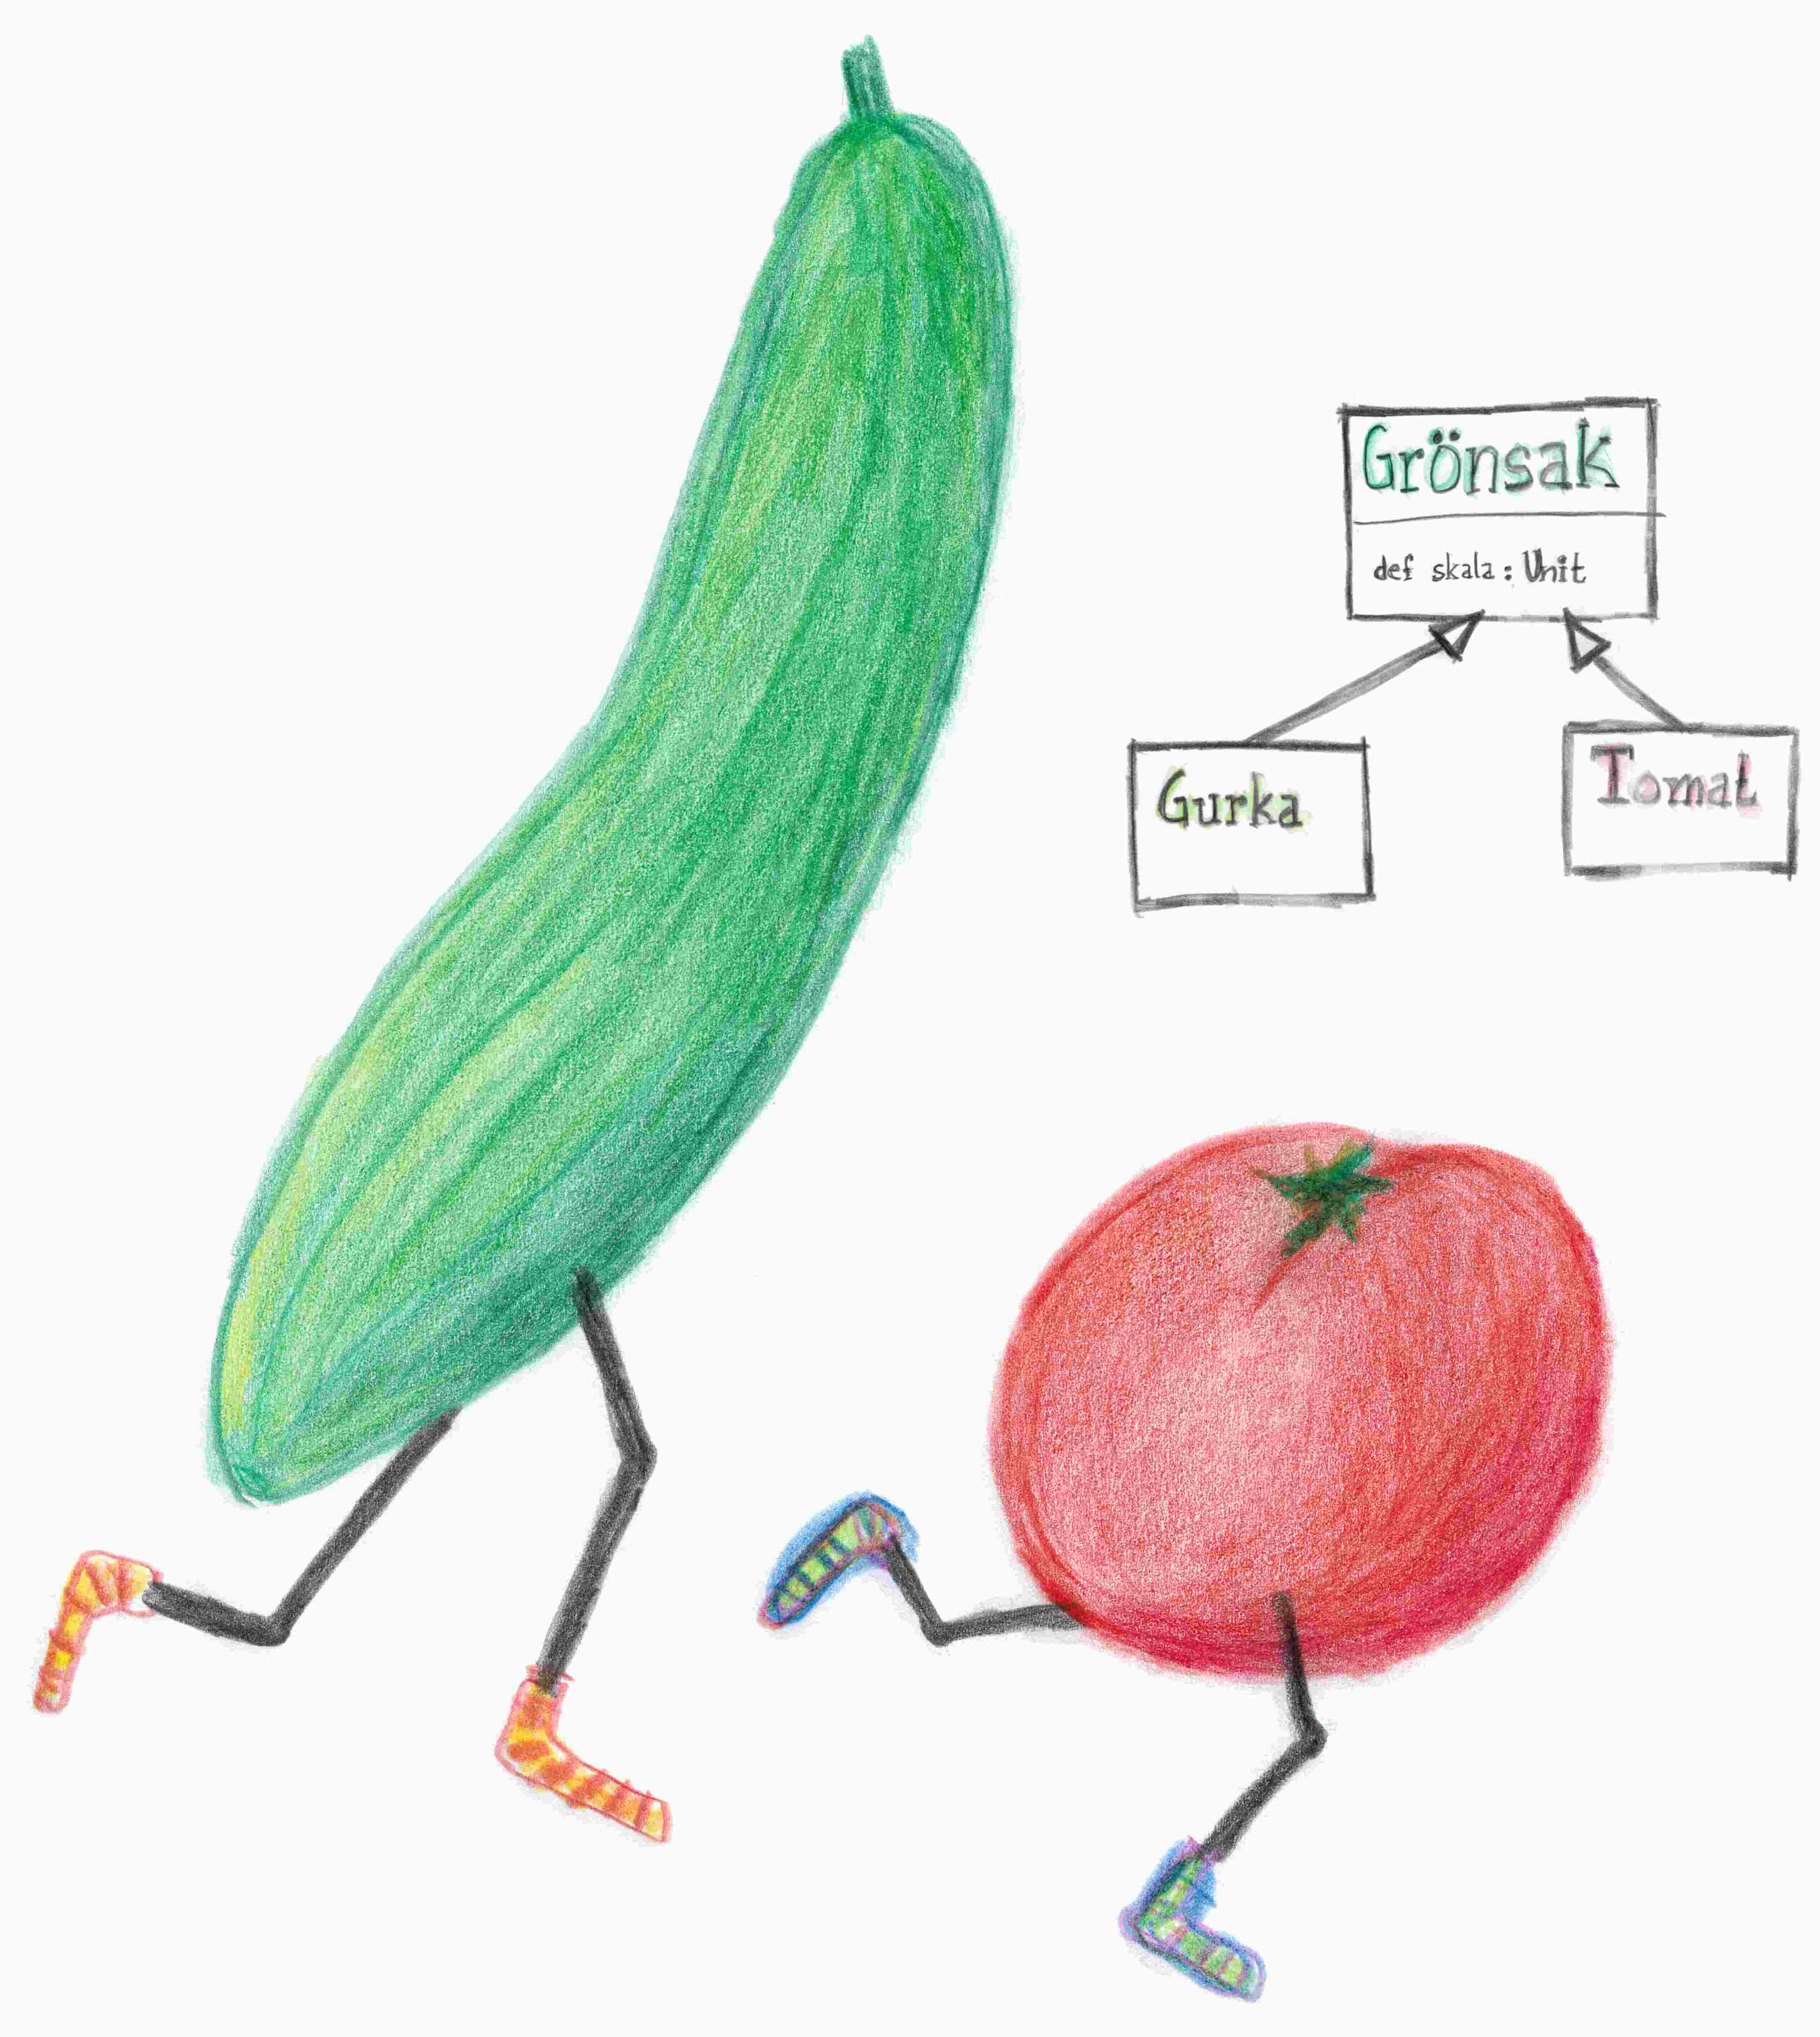
\includegraphics[height=12cm]{cover/gurka.jpg}
}

%\author{Redaktör: Björn Regnell}
\date{\raggedbottom%
\vspace{-2em}\begin{minipage}{1.0\textwidth}\centering
EDAA45, Lp1-2, HT \CurrentYear\\
Datavetenskap, LTH\\
Lunds Universitet\\
~\\
Kompileringsdatum: \today \\
\url{http://cs.lth.se/pgk}
\end{minipage}
}

\usepackage{multicol}

\usepackage{pgffor}  %% http://stackoverflow.com/questions/2561791/iteration-in-latex
                     %  allows:  \foreach \n in {1,...,4}{ do something with \n }

\usepackage{framed}  %  allows:   \begin{framed}\end{framed}
%\newenvironment{Slide}[2][]
%  {\begin{framed}\setlist{noitemsep}\section*{#2}}
%  {\end{framed}}


\newcommand{\SlideHeading}[1]{} %ignore slide headings
\newcommand{\Subsection}[1]{} %ignore slide sections
\newcommand{\SlideOnly}[1]{} %ignore slide font size

\newif\ifkompendium  % to allow conditional text in slides only showing up in compendium
\kompendiumtrue      % in slides: \kompendiumfalse

%!TEX encoding = UTF-8 Unicode

\newcommand{\ModWeekONE}{Introduktion}
\newcommand{\ExeWeekONE}{expressions}
\newcommand{\LabWeekONE}{kojo}


\newcommand{\ModWeekTWO}{Program, kontrollstrukturer}
\newcommand{\ExeWeekTWO}{programs}
\newcommand{\LabWeekTWO}{--}


\newcommand{\ModWeekTHREE}{Funktioner, abstraktion}
\newcommand{\ExeWeekTHREE}{functions}
\newcommand{\LabWeekTHREE}{irritext}


\newcommand{\ModWeekFOUR}{Objekt, inkapsling}
\newcommand{\ExeWeekFOUR}{objects}
\newcommand{\LabWeekFOUR}{blockmole}


\newcommand{\ModWeekFIVE}{Klasser, datamodellering}
\newcommand{\ExeWeekFIVE}{classes}
\newcommand{\LabWeekFIVE}{--}


\newcommand{\ModWeekSIX}{Mönster, felhantering}
\newcommand{\ExeWeekSIX}{patterns}
\newcommand{\LabWeekSIX}{blockbattle}


\newcommand{\ModWeekSEVEN}{Sekvenser, enumerationer}
\newcommand{\ExeWeekSEVEN}{sequences}
\newcommand{\LabWeekSEVEN}{shuffle}


\newcommand{\ModWeekEIGHT}{Matriser, typparametrar}
\newcommand{\ExeWeekEIGHT}{matrices}
\newcommand{\LabWeekEIGHT}{life}


\newcommand{\ModWeekNINE}{Mängder, tabeller}
\newcommand{\ExeWeekNINE}{lookup}
\newcommand{\LabWeekNINE}{words}


\newcommand{\ModWeekTEN}{Arv, komposition}
\newcommand{\ExeWeekTEN}{inheritance}
\newcommand{\LabWeekTEN}{snake0}


\newcommand{\ModWeekELEVEN}{Kontextuella abstraktioner, api}
\newcommand{\ExeWeekELEVEN}{context}
\newcommand{\LabWeekELEVEN}{snake1}


\newcommand{\ModWeekTWELVE}{Valfri fördjupning, Projekt}
\newcommand{\ExeWeekTWELVE}{extra}
\newcommand{\LabWeekTWELVE}{Projekt0}


\newcommand{\ModWeekTHIRTEEN}{Repetition}
\newcommand{\ExeWeekTHIRTEEN}{examprep}
\newcommand{\LabWeekTHIRTEEN}{Projekt1}


\newcommand{\ModWeekFOURTEEN}{Muntligt prov}
\newcommand{\ExeWeekFOURTEEN}{Munta}
\newcommand{\LabWeekFOURTEEN}{Munta}



\newif\ifPreSolution  % to allow tasks and solutions in same file
\PreSolutiontrue      % in solutions: \PreSolutionfalse


\begin{document}

\pagenumbering{roman}
\frontmatter
\maketitle
%!TEX encoding = UTF-8 Unicode
%!TEX root = ../compendium.tex

\clearpage\null\thispagestyle{empty}
\vfill

{
\setlength{\parindent}{0pt}
\emph{Editor}: Björn Regnell \\

%  LIST OF CONTRIBUTORS to https://github.com/lunduniversity/introprog
%    Please contact bjorn.regnell@cs.lth.se if you think you should be
%    on this list, or make a pull request with an update of file briefly
%    describing your contribtion in the commit text.
%    This work is licenced under CC-BY-SA-4.0.
%!TEX encoding = UTF-8 Unicode
%!TEX root = compendium/compendium.tex
\hyphenation{Borg-lund Da-ne-bjer Grampp Palm-qvist Ravn-borg Ro-sen-qvist Schrei-ter Wih-lan-der}
\emph{Contributors} in alphabetical order:
Anders Buhl,
André Philipsson Eriksson,
Anna Axelsson,
Anna Palmqvist Sjövall,
Anton Andersson,
Benjamin Lindberg,
Björn Regnell,
Casper Schreiter,
Cecilia Lindskog,
Dag Hemberg,
Elliot Bräck,
Elsa Cervetti Ogestad,
Emelie Engström,
Emil Wihlander,
Erik Bjäreholt,
Erik Grampp,
Evelyn Beck,
Fredrik Danebjer,
Gustav Cedersjö,
Henrik Olsson,
Hussein Taher,
Jakob Hök,
Jakob Sinclair,
Johan Ravnborg,
Jonas Danebjer,
Jos Rosenqvist,
Maj Stenmark,
Maria Kulesh,
Måns Magnusson,
Nicholas Boyd Isacsson,
Niklas Sandén,
Oliver Persson,
Oscar Sigurdsson,
Oskar Berg,
Oskar Widmark,
Patrik Persson,
Per Holm,
Philip Sadrian,
Sandra Nilsson,
Sebastian Hegardt,
Simon Persson,
Stefan Jonsson,
Theodor Lundqvist,
Tim Borglund,
Tom Postema,
Valthor Halldorsson,
Viktor Claesson,
Wilhelm Wanecek,
William Karlsson.

\\ \newline

\emph{Home}: \url{https://cs.lth.se/pgk} \newline

\emph{Repo}: \url{https://github.com/lunduniversity/introprog} \\ \newline

This compendium is on-going work. \\ \textbf{Contributions are welcome!} \\
\emph{Contact}: \url{bjorn.regnell@cs.lth.se}
\\ \newline

%\emph{Cover art}: Björn Regnell (inspired by Poul Ströyer's illustration of Lennart Hellsing's lyrics to  the childrens song ''Herr Gurka'' with music by Knut Brodin)\\ \newline

~\\ \newline

You can use this work if you respect this \emph{LICENCE}: CC BY-SA 4.0 \\
\url{http://creativecommons.org/licenses/by-sa/4.0/} \\
Please do \emph{not} distribute your solutions to lab assignments and projects.
\\ \newline
Copyright \copyright~ 2015-2017. \\
Dept. of Computer Science, LTH, Lund University. Lund. Sweden.\\
}

%%!TEX encoding = UTF-8 Unicode
%!TEX root = ../compendium.tex

\ChapterUnnum{Framstegsprotokoll} 


\subsubsection*{Genomförda övningar}

\vspace{1em}\noindent 
{Till varje laboration hör en övning med uppgifter som utgör förberedelse inför labben. Du behöver minst behärska grundövningarna för att klara labben inom rimlig tid. Om du känner att du behöver öva mer på grunderna, gör då även extrauppgifterna. Om du vill fördjupa dig, gör fördjupningsuppgifterna som är på mer avancerad nivå. Kryssa för nedan vilka övningar du har gjort, så blir lätt för din handledare att se vilka kunskaper du förvärvat hittills.}

\newcommand{\TickBox}{\raisebox{-.50ex}{\Large$\square$}}
\newcommand{\ExeRow}[1]{\texttt{#1} & \TickBox  &  \TickBox &  \TickBox  \\ \addlinespace }

\begin{table}[h]
\centering
\vspace{2em}
\begin{tabular}{lccc}
\toprule \addlinespace 
{\sffamily\small Övning} & 
{\sffamily\small Grund} &	
{\sffamily\small Extra} &
{\sffamily\small Fördjupning}\\ \addlinespace \midrule \\[-0.7em]
\ExeRow{expressions}
\ExeRow{statements}
\ExeRow{functions}
\ExeRow{data}
\ExeRow{vectors}
\ExeRow{classes}
\ExeRow{traits}
\ExeRow{matching}
\ExeRow{matrices}
\ExeRow{sorting}
\ExeRow{scalajava}
\ExeRow{threads}
\bottomrule
\end{tabular}
\end{table}

\newpage

\subsubsection*{Godkända obligatoriska moment}

\vspace{1em}\noindent 
För att bli godkänd på laborationsuppgifterna och projektuppgiften måste du lösa deluppgifterna och diskutera dina lösningar med en handledare. Denna diskussion är din möjlighet att få feedback på dina lösningar. Ta vara på den!
Se till att handledaren noterar nedan när du blivit godkänd på respektive labb. Spara detta blad tills du fått slutbetyg i kursen. 


\vspace{2.5em}\noindent Namn: \dotfill\\

\vspace{1em}\noindent Namnteckning: \dotfill\\

\newcommand{\LabRow}[1]{\\[-1.1em] \texttt{#1} & \dotfill &  \dotfill  \\ \addlinespace }

\begin{table}[h]
\centering
\vspace{1em}
\begin{tabular}{lcc}
\toprule \addlinespace 
{\sffamily\bfseries\small Lab} & {\sffamily\small Datum gk} &	{\sffamily\small Handledares namnteckning}\\ \addlinespace \midrule \\[-0.5em]
%!TEX encoding = UTF-8 Unicode
%!TEX root = ../compendium2.tex
\LabRow{kojo}
\LabRow{irritext}
\LabRow{blockmole}
\LabRow{blockbattle}
\LabRow{shuffle}
\LabRow{words}
\LabRow{life}
\LabRow{snake}
\LabRow{music}
\LabRow{javatext}
\LabRow{survey}
%\toprule 
\addlinespace \midrule \addlinespace
 \\
{\sffamily\small {\bfseries Projektuppgift} (välj en)	} & \dotfill&\dotfill \\ \addlinespace\addlinespace %\midrule
\texttt{( ) bank}  &  &  \\
\texttt{( ) imageprocessing}  \\
\texttt{( ) tictactoe} \\  
\texttt{( ) }\textit{egendefinerad}  \\
\textit{\small Om egen, ge kort beskrivning:}\\
%\dotfill  \\
\bottomrule
\end{tabular}
\end{table}
%%!TEX root = ../compendium.tex


\ChapterUnnum{Förord} 

Programmering är inte bara ett sätt att ta makten över systemen som styr vårt samhälle. Det är också ett kraftfullt verktyg för tanken. Att lära sig programmering och systemutveckling är första steget på en livslång resa av kontinuerligt lärande. Programmeringsspråk och utvecklingsverktyg kommer och går, men de grundläggande koncepten sekvens, alternativ, repetition och abstraktion som ligger bakom all mjukvara består. 

Detta kompendium utgör kursmaterial för studier i grundläggande programmering, med syfte att ge en solid bas för ingenjörsstudenter och andra som utvecklar system som innehåller mjukvara. 

Kompendiet är framtaget av, med och för studenter och lärare på universitetsnivå, och distribueras som öppen källkod. Det får användas fritt så länge erkännande ges och eventuella ändringar också publiceras som öppen källkod under samma licens som ursprungsmaterialet. På kursens hemsida \href{http://cs.lth.se/pgk}{cs.lth.se/pgk} och repo \href{http://github.com/lunduniversity/introprog}{github.com/lunduniversity/introprog} finns instruktioner om hur du kan bidra till kursmaterialet.

Läromaterialet fokuserar på lärande genom eget arbete och innehåller övningar och laborationer som är organiserade i moduler. Varje modul har ett tema och tillhörande föreläsningsanteckningar.

I kursen används språken Scala och Java för att illustrera grunderna i imperativ och objektorienterad programmering, tillsammans med elementär funktionsprogrammering. Mer avancerad objektorientering och funktionsprogrammering och  lämnas till fortsättningskurser. 



Den kanske viktigaste framgångsfaktorn vid studier i programmering är att bejaka din egen upptäckarglädje och experimentlusta. Det fantastiska med programmering är att dina egna intellektuella konstruktioner faktiskt \emph{gör} något som just \emph{du} har bestämt! Ta vara på det och prova dig fram genom att koda egna idéer -- det är kul när det funkar men minst lika lärorikt är felsökning, buggrättande och alla misslyckade försök som efter hårt arbete vänds till lyckade lösningar och bestående lärdomar. 

Välkommen i programmeringens fascinerande värld och hjärtligt lycka till med dina studier!




\setcounter{tocdepth}{2} % set headings level in table of contents
\tableofcontents
\mainmatter

\pagenumbering{arabic}

%\renewcommand{\section}{\chapter}
\renewcommand{\Lab}[1]{\newpage\chapter{Laboration: {\tt #1}}\label{section:lab:#1}}
\renewcommand{\Teamlab}[1]{\newpage\chapter{Grupplaboration: {\tt #1}}\label{section:lab:#1}}
\renewcommand{\subsection}{\section}

%\renewcommand{\SlideHeading}[1]{\subsection{#1}}  %numbering sections in compendium slides

\part{Första läsperiodens laborationer}

%\toggletrue{IsTask}\togglefalse{IsSolution}

%\chapter{Introduktion}\label{chapter:W01}
\begin{itemize}[nosep]
\item sekvens
\item alternativ
\item repetition
\item abstraktion
\item programmeringsspråk
\item programmeringsparadigmer
\item editera-kompilera-exekvera
\item datorns delar
\item virtuell maskin
\item värde
\item uttryck
\item variabel
\item typ
\item tilldelning
\item namn
\item val
\item var
\item def
\item if
\item else
\item true
\item false
\item MinValue
\item MaxValue
\item aritmetik
\item slumptal
\item math.random
\item logiska uttryck
\item de Morgans lagar
\item while-sats
\item for-sats
\end{itemize}
%!TEX encoding = UTF-8 Unicode
%!TEX root = ../labs.tex

\Lab{\LabWeekONE}
%\externaldocument{compendium}
\begin{Goals}
%!TEX encoding = UTF-8 Unicode

\item Kunna kombinera principerna sekvens, alternativ, repetition, och abstraktion i skapandet av egna program om minst 20 rader kod.
\item Kunna förklara vad ett program gör i termer av sekvens, alternativ, repetition, och abstraktion.
\item Kunna tillämpa principerna sekvens, alternativ, repetition, och abstraktion i enkla algoritmer.
\item Kunna formatera egna program så att de blir lätta att läsa och förstå.
\item Kunna förklara vad en variabel är och kunna skriva deklarationer och göra tilldelningar.
\item Kunna genomföra upprepade varv i cykeln \emph{editera-exekvera-felsöka/förbättra} för att successivt bygga upp allt mer utvecklade program.

\end{Goals}

\begin{Preparations}
\item Repetera veckans föreläsningsmaterial.
\item \DoExercise{\ExeWeekONE}{01}%Gör övning {\tt \ExeWeekONE} i kapitel \ref{exe:W01}.
\item Läs om Kojo i appendix \ref{appendix:kojo}. Kojo Desktop är förinstallerat på LTH:s datorer; om du vill installera Kojo Desktop på din egen dator, följ instruktionerna i \ref{appendix:ide:kojo:install}. Du kan också köra Kojo i din webbläsare här: \url{http://kojo.lu.se/}
\item Läs igenom hela laborationen nedan. Fundera på möjliga lösningar till de uppgifter som är markerade med en penna i marginalen.
% \item Ladda hem och studera översiktligt detta dokument (25 sidor, det räcker att du bläddrar igenom dokumentet och får en uppfattning om hur Kojo kan användas): \\ ''Introduction to Kojo'' \url{http://www.kogics.net/kojo-ebooks#intro}
\end{Preparations}

\subsection{Obligatoriska uppgifter}

Om det förekommer en penna i marginalen ska du anteckna något inför redovisningen.


%%%%%%%%%%%%%%NEDAN ÄR FLYTTAT TILL ÖVNING 1 FÖR ATT GÖRA TYDLIGARE KOPPLING MELLAN LABBAR OCH ÖVN
%\Task \textit{Sekvens}.
%
%\Subtask Starta Kojo. Om du inte redan har svenska menyer: välj svenska i språkmenyn och starta om Kojo.  Skriv in nedan program och tryck på den \emph{gröna} play-knappen.
%
%\begin{Code}
%sudda
%
%fram; höger
%fram; vänster
%färg(grön)
%fram
%\end{Code}
%\noindent
%%Genom att börja din Kojo-program med \code{sudda} så startar du exekveringen i samma utgångsläge: en tom canvas där paddan pekar uppåt, pennan är nere och pennans färg är röd.
%%Då blir det lättare att resonera om vad programmet gör från början till slut, jämfört med om exekveringen beror på resultatet av tidigare exekveringar.
%
%\Subtask\Pen Vad händer om du \emph{inte} börjar programmet med \code{sudda} och kör samma program upprepade gånger? Varför är det bra att börja programmet med \code{sudda}?
%
%\Subtask Rita en kvadrat enligt bilden nedan.
%\vspace{1em}\\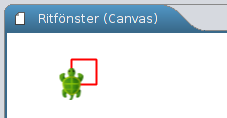
\includegraphics[width=0.45\textwidth]{../img/kojo/kvadrat}
%
%\Subtask Prova olika sätt att skriva din kod \emph{utan} att resultatet ändras: skriv satser i sekvens på flera rader eller satser i sekvens på samma rad med semikolon emellan; använd blanktecken och blanka rader i koden. Hur vill du gruppera dina satser så att de är lätta för en människa att läsa?
%
%\Subtask Prova att ändra på \emph{ordningen} mellan satserna och studera hur resultatet påverkas. Använd den \emph{gula} play-knappen  (programspårning) för att studera exekveringen i detalj. Klicka på satser i ditt program och på rutor i programspårningen och se vad som händer.
%
%
%\Subtask Rita en trappa enligt bilden nedan.
%
%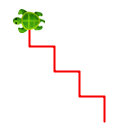
\includegraphics[width=0.2\textwidth]{../img/kojo/stairs}
%
%\Subtask Rita valfri bild på valfri bakgrund med hjälp av några av procedurerna i tabellen nedan. Du kan till exempel rita en rosa triangel med lila konturer mot svart bakgrund. % \ref{lab:kojo:kojo-procedures}.
%Försök att underlätta läsbarheten av din kod med hjälp av lämpliga radbrytningar och gruppering av satser. Undersök hur ordningen av satserna i din kod påverkar resultatet.
%
%
%
%\begin{table}[H]
%\begin{tabular}{l l}\small
%\code|fram(100)| & Paddan går framåt 100 steg (25 om argument saknas).\\
%\code|färg(rosa)| & Sätter pennans färg till rosa. \\
%\code|fyll(lila)| & Sätter ifyllnadsfärgen till lila. \\
%\code|fyll(genomskinlig)| & Gör så att paddan \emph{inte} fyller i något när den ritar. \\
%\code|bredd(20)| & Gör så att pennan får bredden 20. \\
%\code|bakgrund(svart)| & Bakgrundsfärgen blir svart. \\
%\code|bakgrund2(grön,gul)| & Bakgrund med övergång från grönt till gult. \\
%\code|pennaNer|  & Sätter ner paddans penna så att den ritar när den går. \\
%\code|pennaUpp|  & Sänker paddans penna så att den \emph{inte} ritar när den går. \\
%\code|höger(45)|   & Paddan vrider sig 45 grader åt höger. \\
%\code|vänster(45)| & Paddan vrider sig 45 grader åt vänster. \\
%\code|hoppa|       & Paddan hoppar 25 steg utan att rita. \\
%\code|hoppa(100)|  & Paddan hoppar 100 steg utan att rita. \\
%\code|hoppaTill(100, 200)| & Paddan hoppar till läget (100, 200) utan att rita. \\
%\code|gåTill(100, 200)|    & Paddan vrider sig och går till läget (100, 200). \\
%\code|öster|   & Paddan vrider sig så att nosen pekar åt höger. \\
%\code|väster|  & Paddan vrider sig så att nosen pekar åt vänster. \\
%\code|norr|    & Paddan vrider sig så att nosen pekar uppåt. \\
%\code|söder|   & Paddan vrider sig så att nosen pekar neråt. \\
%\code|mot(100,200)|   & Paddan vrider sig så att nosen pekar mot läget (100, 200) \\
%\code|sättVinkel(90)| & Paddan vrider nosen till vinkeln 90 grader. \\
%\end{tabular}
%%\label{lab:kojo:kojo-procedures}
%%\caption{Några användbara procedurer i Kojo.}
%\end{table}


%%% NEDAN ÄR BORTTAGEN FÖR ATT MINSKA MÄNGDEN ARBETE

%\Subtask \emph{Rita och mät}.
%\begin{itemize}[noitemsep]
%\item Börja ditt program med dessa satser:\\ \code{sudda; axesOn; gridOn; sakta(0); osynlig}
%\item Rita sedan en kvadrat som har 444 längdenheter i omkrets.
%\item Ta fram linjalen med höger-klick i ritfönstret och mät så exakt du kan hur lång diagonalen i kvadraten är. Skriv ner resultatet. \\ \emph{Tips:} Du kan zooma med mushjulet om du håller nere Ctrl-knappen. Du kan flytta linjalen om du klick-drar på linjalens skalstreck. Du kan vrida linjalen om du klickar på skalstrecken och håller nere Shift-tangenten.
%\item Kontrollera med hjälp av \code{math.hypot} och \code{println} vad det exakta svaret är. Skriv ner svaret med 3 decimalers noggrannhet. Du kan t.e.x. använda REPL i ett terminalfönster bredvid, eller öppna ett nytt extra Kojo-fönster i Arkiv-menyn, eller lägga in utskrifterna sist i ditt befintliga program. Utskrifter med \code{println} i Kojo sker i utdatafönstret.
%\end{itemize}
%
%\Subtask Rita en liksidig triangel med sidan 300 längdenheter genom att ge lämpliga argument till \code{fram} och \code{höger}. Vinklar anges i grader.
%
%\Subtask\Checkpoint Visa dina resultat för en handledare och diskutera hur uppgifterna ovan illustrerar principen om sekvens.

\vspace{1em}

% \Task Läs om hur du gör grafikprogram med Kojo i Appendix \ref{appendix:kojo} och övning {\tt \ExeWeekONE} i kapitel \ref{exe:W01}.


\Task \textit{Sekvens och repetition}. Rita en kvadrat med hjälp av \code+upprepa(n){ ??? }+ där du ersätter \code{n} med antalet repetitioner och \code{???} med de satser som ska repeteras.

%\Subtask Om du kör Kojo Desktop: Prova att köra ditt program med den \emph{gula} play-knappen för programspårning. Studera exekveringssekvensen. Klicka på anropen i programspårningsfönstret och studera markeringarna i ritfönstret.





\Task \textit{Variabel och repetition}.

\Subtask Funktionen \code{System.currentTimeMillis} ingår i Javas standardbibliotek och ger ett heltal av typen \code{Long} med det nuvarande antalet millisekunder sedan midnatt den första januari 1970.  Med Kojo-proceduren \code{sakta(0)} blir det ingen fördröjning när paddan ritar och utritningen sker så snabbt som möjligt. Prova nedan program och förklara vad som händer.
\begin{Code}
sakta(0)
val n = 800 * 4
val t1 = System.currentTimeMillis
upprepa(n){ upprepa(4){ fram; höger } }
val t2 = System.currentTimeMillis
println(s"$n kvadratvarv tog ${t2 - t1} millisekunder")
\end{Code}
\noindent Om du kör Kojo Desktop är det bra att börjar programmet med \code{sudda}. (Varför?)

\Subtask\Pen Anteckna ungefär hur många kvadratvarv per sekund som paddan kan rita när den är som snabbast. Kör flera gånger eftersom den virtuella maskinen behöver ''värmas upp'' för att maskinkoden ska optimeras. Vissa körningar kan gå långsammare om skräpsamlaren behöver lägga tid på att frigöra minne.

\Subtask\Pen Vad har variablerna i koden ovan för namn? Vad har variablerna för värden?

\Subtask Rita en kvadrat igen, men nu med hjälp av en \code{while}-sats och en loopvariabel. %Studera exekveringen med programspårning (den gula play-knappen).

\begin{Code}
sakta(100)
var i = 0
while (???) { fram; höger; i = ??? }
\end{Code}

\Subtask\Pen Vad är det för skillnad på variabler som deklareras med \code{val} respektive \code{var}?

\Subtask Rita en kvadrat igen, men nu med hjälp av en \code{for}-sats. Skriv ut värdet på den lokala variabeln \code{i} i varje loop-runda.

\begin{Code}
for (i <- 1 to ???) { ??? }
\end{Code}

\Subtask\Pen Går det att tilldela variabeln \code{i} ett nytt värde i loopen?

\Subtask\Pen Går det att referera till namnet \code{i} utanför loopen?


\Subtask Rita en kvadrat igen, men nu med hjälp av \code{foreach}. Skriv ut loopvariabelns värde i varje runda.

\begin{Code}
(1 to ???).foreach{ i => ??? }
\end{Code}

%\Subtask\Pen För var och en av de fyra repetitionskonstruktionerna du sett ovan, \code{upprepa}, \code{while}, \code{for} och \code{foreach}: skriv kod med penna på papper som skriver ut de första 100 jämna heltalen med blanktecken emellan: \code{2 4 6 8 10 12 ...} etc.\\ Vilken typ av loop tycker du är enklast att använda i detta fall?


\Task \textit{Abstraktion}.

\Subtask Använd en repetition för att abstrahera nedan sekvens, så att programmet blir kortare:
\begin{Code}
fram; höger; hoppa; fram; vänster; hoppa; fram; höger;
hoppa; fram; vänster; hoppa; fram; höger; hoppa; fram;
vänster; hoppa; fram; höger; hoppa; fram; vänster; hoppa;
fram; höger; hoppa; fram; vänster; hoppa
\end{Code}

%\Subtask\Pen Sök på nätet efter ''DRY principle programming'' och beskriv med egna ord vad DRY betyder och varför det är en viktig princip.

\Subtask Definiera en egen procedur som heter \code{kvadrat} med hjälp av nyckelordet \code{def} som vid anrop ritar en kvadrat med hjälp av en \code{for}-loop.

\begin{Code}
def kvadrat = for (???) {???}
\end{Code}


\Subtask Anropa din abstraktion efter att den deklarerats och efter att du exekverat:\\\code{sakta(100)}


\Subtask Anropa din abstraktion inuti en \code{for}-loop så att paddan ritar en stapel som är 10 kvadrater hög enligt bilden nedan.

\begin{figure}
  \begin{multicols}{2}

  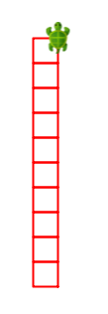
\includegraphics[scale=0.6]{../img/kojo/square-column}

  \columnbreak

  \begin{Code}
  def kvadrat = for (???) {???}
  for (???) {???}
  \end{Code}

  \end{multicols}
  \caption{En kvadratstapel.\label{fig:kojo-lab:column}}
\end{figure}

\Subtask %Kör ditt program med den \emph{gula} play-knappen. 
Studera hur anrop av proceduren \code{kvadrat} påverkar exekveringssekvensen av dina satser genom att göra lämpliga utskrifter så att du kan se när olika delar av koden exekveras. Vid vilka punkter i programmet sker ett ''hopp'' i sekvensen i stället för att efterföljande sats exekveras?  Använd lämpligt argument till \code{sakta} för att du ska hinna studera exekveringen.


\Subtask Rita samma bild med 10 staplade kvadrater (se bild \ref{fig:kojo-lab:column} på sidan \pageref{fig:kojo-lab:column}), men nu \emph{utan} att använda abstraktionen \code{kvadrat} -- använd i stället en nästlad repetition (alltså en upprepning inuti en upprepning). Vilket av de två sätten (med och utan abstraktionen \code{kvadrat}) är lättast att läsa? %\emph{Tips:} Varje gång du trycker på någon av play-knapparna, sparas ditt program. Du kan se dina sparade program om du klickar på \emph{Historik}-fliken. Du kan också stega bakåt och framåt i historiken med de blå pilarna bredvid play-knapparna.

\Subtask Generalisera din abstraktion \code{kvadrat} genom att ge den en parameter \code{sida: Double} som anger hur stor kvadraten blir. Rita flera kvadrater i likhet med bild \ref{fig:kojo-lab:resize} på sidan \pageref{fig:kojo-lab:resize}).

\begin{figure}[H]

\includegraphics{../img/kojo/square-param}
  \caption{Olika stora kvadrater.\label{fig:kojo-lab:resize}}

\end{figure}



%\Subtask\Pen%\Checkpoint
%Se över ditt program i föregående uppgift och säkerställ att det är lättläst och följer en struktur som börjar med alla definitioner i logisk ordning och därefter fortsätter med huvudprogrammet.
%%Diskutera ditt program med en handledare.



%\Subtask\Pen Spara ditt program i en fil men lämpligt namn och ha programmet redo när det är din tur att redovisa vad du gjort under laborationen.
%Anteckna några åtgärder du vidtagit för att göra programmet mer lättläst.







\Task \emph{Alternativ.} \label{kojo:alt}

\Subtask Kör programmet nedan. Förklara vad som händer. %Använd den gula play-knappen för att studera exekveringen.

\begin{Code}
sakta(5000)

def move(key: Int): Unit = {
  println("key: " + key)
  if (key == 87) fram(10)
  else if (key == 83) fram(-10)
}

move(87); move('W'); move('W')
move(83); move('S'); move('S'); move('S')
\end{Code}

\Subtask \label{subtask:keypress}  Kör programmet nedan. Notera \code{activateCanvas} för att du ska slippa klicka i ritfönstret innan du kan styra paddan. Anropet \code{onKeyPress(move)} gör så att \code{move} kommer att anropas då en tangent trycks ned. Lägg till kod i \code{move} som gör att tangenten A ger en vridning moturs med 5 grader medan tangenten D ger en vridning medurs 5 grader. Med \code{onKeyPress} bestämmer man vilken procedur som ska köras vid tangenttryck.

\begin{Code}
sakta(0); activateCanvas

def move(key: Int): Unit = {
  println("key: " + key)
  if (key == 'W') fram(10)
  else if (key == 'S') fram(-10)
}

onKeyPress(move)
\end{Code}



%\Subtask Spara ditt program i en fil men lämpligt namn och ha programmet redo när det är din tur att redovisa vad du gjort under laborationen.


\subsection{Kontrollfrågor}\Checkpoint

\noindent Repetera teorin för denna vecka och var beredd på att kunna svara på dessa frågor när det blir din tur att redovisa vad du gjort under laborationen:

\begin{enumerate}
\item Vad innebär sekventiell exekvering av satser?
\item Vad är skillnaden mellan en sats och ett uttryck?
\item Vad är skillnaden mellan en procedur och en funktion?
\item Spelar ordningen mellan argument någon roll vid anrop av en funktion med flera parametrar?
\item Vad är en variabel? Ge exempel på deklaration, initialisering och tilldelning av variabler, samt användning av variabler i uttryck.
\item Vad är ett logiskt uttryck? Ge exempel på användning av logiska uttryck.
\item Vad är abstraktion? Ge exempel på användning av abstraktion.
\item Vad är nyttan med abstraktion?
\item Vad innebär sidoeffekt? Förklara och ge exempel.
\item Hur deklareras och initialiseras en variabel vars värde är förändringsbart?
\item Hur deklareras och initialiseras en variabel vars värde är oföränderligt?
\item Är det ett körtidsfel eller kompileringsfel att tilldela en oföränderlig variabel ett nytt värde?
\item Ange vilken av \code{for} och \code{while} som är lämpligast i dessa fall:
\begin{itemize}[noitemsep, nolistsep]
\item[A.] Summera de hundra första heltalen.
\item[B.] Räkna antal tecken i en sträng innan första blanktecken.
\item[C.] Dra 100 slumptal mellan 1 och 6 och summera de tal som är mindre än 3.
\item[D.] Summera de första heltalen från 1 och uppåt tills summan är minst 100.
\end{itemize}
\end{enumerate}


\subsection{Frivilliga extrauppgifter}

\noindent Gör i mån intresse och träningsbehov nedan uppgifter i valfri ordning.

\Task \emph{Abstraktion och generalisering}.

\Subtask Skapa en abstraktion \code{def stapel = ???} som använder din abstraktion \code{kvadrat}.

\Subtask Du ska nu \emph{generalisera} din procedur så att den inte bara kan rita exakt 10 kvadrater i en stapel. Ge proceduren \code{stapel} en parameter \code{n} som styr hur många kvadrater som ritas.
\begin{Code}
def kvadrat = ???
def stapel(n: Int) = ???

sakta(100)
stapel(42)
\end{Code}



\Subtask Rita nedan bild med hjälp av abstraktionen \code{stapel}. Det är totalt 100 kvadrater och varje kvadrat har sidan 25. \emph{Tips:} Med ett negativt argument till procedur \code{hoppa} kan du få sköldpaddan att hoppa baklänges utan att rita, t.ex. \code{hoppa(-10*25)}

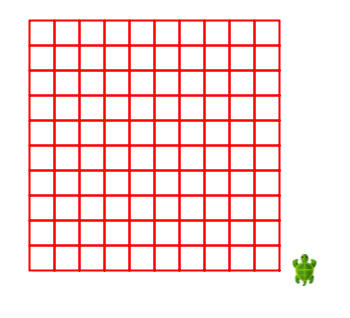
\includegraphics[width=0.3\textwidth]{../img/kojo/square-grid}

\Subtask Generalisera dina abstraktioner \code{kvadrat} och \code{stapel} så att man kan påverka storleken på kvadraterna som ritas ut.

\Subtask Skapa en abstraktion \code{rutnät} med lämpliga parametrar som gör att man kan rita rutnät med olika stora kvadrater och olika många kvadrater i både x- och y-led.

\Subtask Generalisera dina abstraktioner \code{kvadrat} och \code{stapel} så att man kan påverka fyllfärgen och pennfärgen för kvadraterna som ritas ut.

\Task \emph{Växling med booleska värden.}

\Subtask Bygg vidare på programmet i uppgift \ref{kojo:alt} och lägg till nedan kod i början av programmet. Lägg även till kod som gör så att om man trycker på tangenten G så sätts rutnätet omväxlande på och av. Observera att det är exakt \emph{en} procedur som anropas vid \code{onKeyPress}.

\begin{Code}
var isGridOn = false

def toggleGrid =
  if (isGridOn) {
    gridOff
    isGridOn = false
  } else {
    gridOn
    isGridOn = true
  }
\end{Code}

\Subtask Gör så att när man trycker på tangenten X så sätter man omväxlande på och av koordinataxlarna. Använd en variabel \code{isAxesOn} och definiera en abstraktion \code{toggleAxes} som anropar \code{axesOn} och \code{axesOff} på liknande sätt som i föregående uppgift.


\Task \emph{Repetition.}~Skriv en procedur \code{randomWalk} med detta huvud: \\
\code{def randomWalk(n: Int, maxStep: Int, maxAngle: Int): Unit}\\ som gör så att paddan tar \code{n} steg av slumpmässig längd mellan \code{0} och \code{maxStep}, samt efter varje steg vrider sig åt vänster en slumpmässig vinkel mellan \code{0} och \code{maxAngle}. Anropa din procedur med olika argument och undersök hur dess värden påverkar bildens utseende. \emph{Tips:} Uttrycket \code{math.random() * 100} ger ett tal från 0 till (nästan) 100. Du kan styra hur långsamt paddan ritar genom anrop av \code{sakta(???)} (prova dig fram till något  lämpligt heltalsargument i stället för \code{???}).
\vspace{2em}\\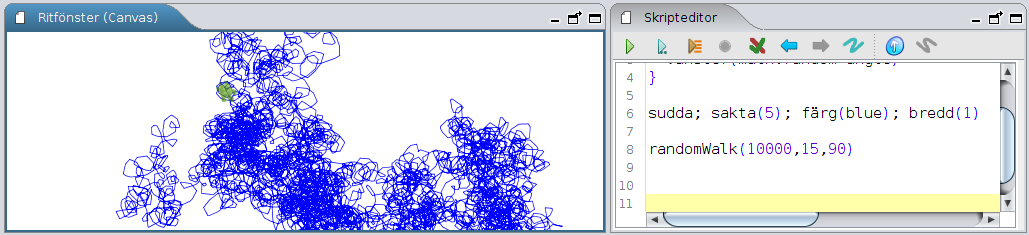
\includegraphics[width=\textwidth]{../img/kojo/random-walk.png}


\Task \emph{Variabler, namngivning och formatering.}

\Subtask Klistra in nedan konstigt formatterade program \emph{exakt} som det står med blanktecken, indragningar och radbrytningar. Kör programmet och förklara vad som händer.

\begin{figure}[H]
\begin{Code}
// Ett konstigt formaterat program med en del konstiga namn.

def gurka(x: Double,
y: Double, namn: String,
typ: String,
värde:String) = {
val tomat = 15
val h = 30
hoppaTill(x,y)
norr
skriv(namn+": "+typ)
hoppaTill(x+tomat*(namn.size+typ.size),y)
skriv(värde); söder; fram(h); vänster
fram(tomat * värde.size); vänster
fram(h); vänster
fram(tomat * värde.size); vänster }
sudda; färg(svart); val s = 130
val h = 40
var x = 42; gurka(10, s-h*0, "x","Int", x.toString)
var y = x; gurka(10, s-h*1, "y","Int", y.toString)
x = x + 1; gurka(10, s-h*2, "x","Int", x.toString)
gurka(10, s-h*3, "y","Int", y.toString); osynlig
\end{Code}
\end{figure}

\Subtask\Pen Skriv ner namnet på alla variabler som förekommer i programmet.

\Subtask\Pen Vilka av dessa variabler är lokala?

\Subtask\Pen Vilka av dessa variabler kan förändras efter initialisering?

\Subtask\Pen Föreslå tre förändringar av programmet ovan (till exempel namnbyten) som gör att det blir lättare att läsa och förstå.

\Subtask Gör sök-ersätt av \code{gurka} till ett bättre namn. \emph{Tips:} undersök kontextmenyn i editorn i Kojo genom att högerklicka. Använd kortkommandot för Sök/Ersätt.

\Subtask Gör automatisk formatering av koden med hjälp av lämpligt kortkommando. Notera skillnaderna. Vilka autoformateringar gör programmet lättare att läsa? Vilka manuella formateringar tycker du bör göras för att öka läsbarheten? Ge funktionen \code{gurka} ett bättre namn.  Diskutera läsbarheten med en handledare.



\Task \label{task:measuretime} \emph{Tidmätning.} Hur snabb är din dator?

\Subtask \label{task:timer} Skriv in koden nedan i Kojos editor och kör upprepade gånger med den gröna play-knappen. Tar det lika lång tid varje gång? Varför?

\begin{Code}
object timer {
  def now: Long = System.currentTimeMillis
  var saved: Long = now
  def elapsedMillis: Long = now - saved
  def elapsedSeconds: Double = elapsedMillis / 1000.0
  def reset: Unit = { saved = now }
}

// HUVUDPROGRAM:
timer.reset
var i = 0L
while (i < 1e8.toLong) { i += 1 }
val t = timer.elapsedSeconds
println("Räknade till " + i + " på " + t + " sekunder.")
\end{Code}


\Subtask Ändra i loopen i uppgift \ref{task:timer}) så att den räknar till 4.4 miljarder. Hur lång tid tar det för din dator att räkna så långt?\footnote{Det går att göra ungefär en heltalsaddition per klockcykel per kärna. Den första elektroniska datorn \href{https://sv.wikipedia.org/wiki/ENIAC}{Eniac} hade en klockfrekvens motsvarande 5 kHz. Den dator på vilken denna övningsuppgift skapades hade en i7-4790K turboklockad upp till 4.4 GHz.
%\href{http://www.extremetech.com/computing/185512-overclocking-intels-core-i7-4790k-can-devils-canyon-fix-haswells-low-clock-speeds/2}{www.extremetech.com/computing/185512-overclocking-intels-core-i7-4790k-can-devils-canyon-fix-haswells-low-clock-speeds/2}
}

\Subtask  Om du kör på en Linux-maskin: Kör nedan Linux-kommando upprepade gånger i ett terminalfönster. Med hur många MHz kör din dators klocka för tillfället? Hur förhåller sig klockfrekvensen till antalet rundor i while-loopen i föregående uppgift? (Det kan hända att din dator kan variera centralprocessorns klockfrekvens. Prova både medan du kör tidmätningen i Kojo och då din dator ''vilar''. Vad är det för poäng med att en processor kan variera sin klockfrekvens?)
\begin{REPLnonum}
> lscpu | grep MHz
\end{REPLnonum}


\Subtask Ändra i koden i uppgift \ref{task:timer}) så att \code{while}-loopen bara kör 5 gånger. %Kör programmet med den \emph{gula} play-knappen. Scrolla i programspårningen och förklara vad som händer. Klicka på \code{CALL}-rutorna och se vilken rad som markeras i ditt program.

\Subtask Lägg till koden nedan i ditt program och försök ta reda på ungefär hur långt din dator hinner räkna till på en sekund för \code{Long}- respektive \code{Int}-variabler. Använd den gröna play-knappen.
\begin{CodeSmall}
def timeLong(n: Long): Double = {
  timer.reset
  var i = 0L
  while (i < n) { i += 1 }
  timer.elapsedSeconds
}

def timeInt(n: Int): Double = {
  timer.reset
  var i = 0
  while (i < n) { i += 1 }
  timer.elapsedSeconds
}

def show(msg: String, sec: Double): Unit = {
  print(msg + ": ")
  println(sec + " seconds")
}

def report(n: Long): Unit = {
  show("Long " + n, timeLong(n))
  if (n <= Int.MaxValue) show("Int  " + n, timeInt(n.toInt))
}

// HUVUDPROGRAM, mätningar:

report(Int.MaxValue)
for (i <- 1 to 10) report(4.26e9.toLong)
\end{CodeSmall}

\Subtask Hur mycket snabbare går det att räkna med \code{Int}-variabler jämfört med \code{Long}-variabler? Diskutera gärna svaret med en handledare.

\Task Lek med färg i Kojo. Sök på internet efter dokumentationen för klassen \code{java.awt.Color} och studera vilka heltalsparametrar den sista konstruktorn i listan med konstruktorer tar för att skapa sRGB-färger. Om du högerklickar i editorn i Kojo och väljer ''Välj färg...'' får du fram färgväljaren och med den kan du välja fördefinierade färger eller blanda egna färger. När du har valt färg får du se vilka parametrar till \code{java.awt.Color} som skapar färgen. Testa detta i REPL:

\begin{REPL}
scala> val c = new java.awt.Color(124,10,78,100)
c: java.awt.Color = java.awt.Color[r=124,g=10,b=78]

scala> c.  // tryck på TAB
asInstanceOf    getColorComponents      getRGBComponents
brighter        getColorSpace           getRed
createContext   getComponents           getTransparency
darker          getGreen                isInstanceOf
getAlpha        getRGB                  toString
getBlue         getRGBColorComponents

scala> c.getAlpha
res3: Int = 100
\end{REPL}
Skriv ett program som ritar många figurer med olika färger, till exempel cirklar som nedan. Om du använder alfakanalen blir färgerna genomskinliga.

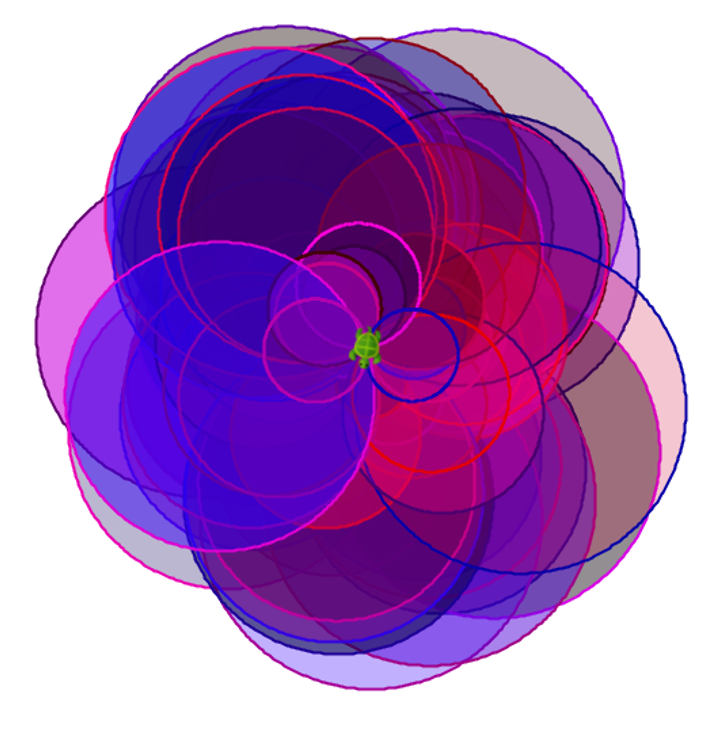
\includegraphics[width=0.82\textwidth]{../img/kojo/random-color-circles.png}


\Task Ladda ner ''Uppdrag med Kojo'' från \href{http://lth.se/programmera/uppdrag}{lth.se/programmera/uppdrag}  och gör några uppgifter som du tycker verkar intressanta.

%\Subtask ''Programming Fundamentals with Kojo'' som kan laddas ner här:\\
%\href{http://wiki.kogics.net/kojo-codeactive-books}{wiki.kogics.net/kojo-codeactive-books}

\Task Om du vill jobba med att hjälpa skolbarn att lära sig programmera med Kojo, kontakta \url{http://www.vattenhallen.lth.se} och anmäl ditt intresse att vara handledare.


%\chapter{Kodstrukturer}\label{chapter:W02}
\begin{itemize}[nosep]
\item samling: Range
\item for-uttryck
\item map
\item foreach
\item flatMap
\item algoritm vs implementation
\item pseudokod
\item algoritm: swap
\item algoritm: summering
\item algoritm: min/max
\item paket
\item import
\item filstruktur
\item jar
\item dokumentation
\item programlayout
\item JDK
\item konstanter vs föränderlighet
\item objektorientering
\item klasser
\item objekt
\item punktnotation
\item referensvariabler
\item referenstilldelning
\item anropa metoder
\item block
\item namnsynlighet
\item namnöverskuggning
\item SimpleWindow
\end{itemize}
%%!TEX encoding = UTF-8 Unicode
%!TEX root = ../compendium2.tex

% INGEN LAB DENNA VECKA


\setcounter{chapter}{2}

%\chapter{Funktioner, Objekt}\label{chapter:W03}
Koncept du ska lära dig denna vecka:
\begin{multicols}{2}\begin{itemize}[nosep,label={$\square$},leftmargin=*]
\item definera funktion
\item anropa funktion
\item parameter
\item returtyp
\item värdeandrop
\item namnanrop
\item default-argument
\item namngivna argument
\item applicera funktion på alla element i en samling
\item procedur
\item värdeanrop vs namnanrop
\item uppdelad parameterlista
\item skapa egen kontrollstruktur
\item objekt
\item modul
\item punktnotation
\item tillstånd
\item metod
\item medlem
\item funktionsvärde
\item funktionstyp
\item äkta funktion
\item stegad funktion
\item apply
\item lazy val
\item lokala funktioner
\item aktiveringspost
\item rekursion
\item basfall
\item anropsstacken
\item objektheapen
\item cslib.window.SimpleWindow\end{itemize}\end{multicols}

%!TEX encoding = UTF-8 Unicode
%!TEX root = ../compendium2.tex

\Lab{\LabWeekTHREE}
\begin{Goals}
%!TEX encoding = UTF-8 Unicode
%!TEX root = ../compendium2.tex

%\item Kunna kompilera Scalaprogram med \texttt{scalac}.
%\item Kunna köra Scalaprogram med \texttt{scala}.
%\item Kunna definiera och anropa funktioner.
%\item Kunna använda och förstå default-argument.
%\item Kunna ange argument med parameternamn.
\item Kunna skapa ett större program med din egen kod efter dina egna idéer.
\item Kunna använda en editor och terminalen för att iterativt editera, kompilera, och testa din kod.
\item Kunna använda variabler i kombination med alternativ och repetetition i flera nivåer.
\item Kunna stegvis förbättra din kod för att underlätta förändring och öka läsbarhet.
\item Kunna skapa och använda abstraktioner för att generalisera och möjliggöra återanvändning av kod.

\end{Goals}

\begin{Preparations}
\item \DoExercise{\ExeWeekTWO}{02}
\item \DoExercise{\ExeWeekTHREE}{03}
\end{Preparations}



\subsection{Obligatoriska uppgifter}


\begin{quote}
\textbf{Blockmullvad} (\textit{Talpa laterculus}) är ett fantasidjur i familjen mullvadsdjur.
Den är känd för sitt karaktäristiska kvadratiska utseende.
Den lever mest ensam i sina underjordiska gångar som till skillnad från mullvadens (\emph{Talpa europaea}) har helt raka väggar.
\end{quote}

\begin{figure}
\end{figure}

\Task
Du ska skriva ett Scala-program med en vanlig texteditor och kompilera ditt program med kommandot \texttt{scalac} och sedan köra programmet med kommandot \texttt{scala}.

\Subtask
Öppna en texteditor, till exempel gedit eller Atom (se appendix~\ref{appendix:edit} för hjälp).
Skapa en ny fil med namnet \texttt{Mole.scala} och spara den i en ny katalog i din hemkatalog, till exempel \texttt{\textasciitilde/pgk/mole/Mole.scala}, där \texttt{\textasciitilde} är din hemkatalog.

\Subtask
Öppna ett terminalfönster (se appendix~\ref{appendix:terminal} för hjälp).
Navigera till din nya katalog med \texttt{cd}-kommandot \Eng{change directory} och kontrollera med \texttt{ls}-kommandot \Eng{list} att din nya fil finns där.
\begin{REPLnonum}
> cd ~/pgk/mole
> ls
\end{REPLnonum}
Om allt går bra ska \texttt{ls}-kommandot skriva ut \texttt{Mole.scala}.

\Subtask
Gå tillbaka till din texteditor och skriv in ett objekt med namnet \code{Mole} i din fil.
Lägg till en \code{main}-funktion i objektet som skriver ut texten \emph{Keep on digging!} med hjälp av funktionen \code{println}.
Behöver du hjälp kan du gå tillbaka till övningarna i kapitel~\ref{exe:W03}.

\Subtask
Kör kommandot \texttt{scalac Mole.scala} i terminalfönstret för att kompilera ditt program.
Om kompilatorn rapporterar några fel rättar du till det i din texteditor kompilerar igen.
Kontrollera sedan med \texttt{ls}-kommandot att några filer som slutar på \texttt{class} har skapats.

\Subtask
Kör kommandot \texttt{scala Mole} för att köra ditt program.
Om att går bra ska texten du angivit skrivas ut i terminalfönstret.


\Task
Nu har du skrivit ett Scala-program som skriver ut en uppmaning till en mullvad att fortsätta gräva.
Det programmet är inte så användbart, eftersom mullvadar inte kan inte läsa.
Nästa steg är att skriva ett grafiskt program, snarare än ett textbaserat.

Funktionen \code{println} som anropas i \code{main}-funktionen ingår i Scalas standardbibliotek.
Ett programbibliotek innehåller kod eller kompilerade programsnuttar som kan användas av andra program, och för de flesta programspråk ingår ett standardbibliotek som alla program kan nyttja.
Till grafiken i denna uppgift ska du använda ett bibliotek som kallas \emph{cslib} och som kommer att användas även i senare labbar.

\Subtask

Ladda ner \texttt{cslib.jar} via länken \url{http://cs.lth.se/pgk/cslib} och lägg jar-filen i samma katalog som ditt Scala-program.
En jar-fil används för att paketera färdigkompilerade program, kod, dokumentation, resursfiler, etc, och är komprimerad på samma sätt som en zip-fil.

\Subtask
Byt ut \code{main}-funktionens kropp mot följande block:
\begin{Code}
{
	val w = new cslib.window.SimpleWindow(300, 500, "Digging")
	w.moveTo(10, 10)
	w.lineTo(10, 20)
	w.lineTo(20, 20)
	w.lineTo(20, 10)
	w.lineTo(10, 10)
}
\end{Code}
Den första raden skapar ett nytt \code{SimpleWindow} som ritar upp ett fönster som är 300 bildpunkter brett och 500 bildpunkter högt med titeln \emph{Digging}.
\code{SimpleWindow} har en \emph{penna} som kan flyttas runt och rita linjer.
Anropet \code{w.moveTo(10, 10)} flyttar pennan för fönstret \code{w} till position $(10,10)$ utan att rita något, och anropet \code{w.lineTo(10, 20)} ritar en linje därifrån till position $(10, 20)$.

\Subtask
Nu ska du kompilera ditt program, men eftersom \code{SimpleWindow} inte finns i Scalas standardbibliotek utan i \texttt{cslib.jar} behöver du visa kompilatorn var den ska leta.
Det gör du genom att ange en \emph{classpath}, dvs. en sökväg till \texttt{class}-filer, när du kompilerar.
Använd flaggan \texttt{-cp cslib.jar} för att ange \texttt{cslib.jar} som classpath och kompilera ditt Scala-program igen:
\begin{REPLnonum}
> scalac -cp cslib.jar Mole.scala
\end{REPLnonum}

\Subtask
Nu ska du köra ditt program, och då behöver du också ange var \texttt{class}-filerna ligger.
Du ska ange den katalog där \texttt{class}-filerna för \code{Mole} ligger, som du just kompilerat, men du ska också ange \texttt{cslib.jar}, och det gör du med en kolon-separerad lista\footnote{Kolon används i Linux och macOS, medan Windows använder semikolon.}, till exempel \code{"sökväg1:sökväg2:sökväg3"}.
Katalogen du står i, där dina \texttt{class}-filer ligger, kan anges med en punkt (\texttt{.}).
Kör programmet med följande kommando (om Windows använd semikolon):
\begin{REPLnonum}
> scala -cp ".:cslib.jar" Mole
\end{REPLnonum}
Du ska nu få upp ett fönster med en liten kvadrat utritad i övre vänstra hörnet.


\Task
Hela ditt program är för tillfället samlat i en och samma funktion, vilket fungerar bra för väldigt små program.
Nu ska vi strukturera programmet så det blir lättare att återanvända samma kodsnuttar.

\Subtask
Lägg till ett objekt med namnet \code{Graphics} i \texttt{Mole.scala} och flytta dit deklarationen av fönstret \code{w}.
Skapa en ny funktion med namnet \code{square} i det nya objektet och flytta dit koden som ritar kvadraten.
Anropa \code{square} i din \code{main}-funktion.
Filen \texttt{Mole.scala} ska se ut såhär (förutom \code{???}):
\begin{Code}
object Graphics {
	val w = new cslib.window.SimpleWindow(300, 500, "Digging")
	def square(): Unit = ???
}
object Mole {
	def main(args: Array[String]): Unit = {
		Graphics.square()
	}
}
\end{Code}
Observera att du inte kan anropa \code{square} direkt i funktionen \code{main}, utan måste ange att det är \code{square}-funktionen inuti \code{Graphics} du vill anropa.

\Subtask
Kompilera \texttt{Mole.scala} med \texttt{scalac}.
Glöm inte att ange korrekt classpath.
(\emph{Tips:} Du kan trycka uppåtpil för att komma till tidigare kommandon i terminalen.)
Kontrollera med \texttt{ls} att det nu också finns \texttt{class}-filer för \code{Graphics}-objektet.

\Subtask
Kör programmet \code{Mole} med \texttt{scala}.
Glöm inte att ange korrekt classpath.
Om allt fungerar ska programmet göra samma sak som innan.

\Task
Nu har du gjort ett grafiskt program, men ännu syns ingen mullvad.
Det är dags att ta reda på hur koordinatsystemet fungerar i denna grafiska miljö, så vi kan få mullvaden att hitta rätt.

\Subtask
Ändra i \code{Graphics.square} så att kvadraten ritas upp i \emph{övre högra} hörnet istället.
Prova dig fram för att ta reda på hur koordinatsystemet fungerar genom att ändra i koden, kompilera och köra programmet tills du får rätt på det.

\Subtask\Checkpoint
Visa kvadraten för din labbhandledare och förklara vad de två parametrarna gör genom att peka ut ungefär var positionerna $(0,0)$, $(300, 0)$, $(0, 300)$ och $(300, 300)$ ligger.

\Subtask
Ta bort anropet till funktionen \code{square} när du har visat den för din labbhandledare.

\Task
Nu ska du skapa ett nytt koordinatsystem för \code{Graphics} som har \emph{stora} bildpunkter.
Vi kallar \code{Graphics} stora bildpunkter för \emph{block} för att lättare skilja dem från \code{SimpleWindow}s bildpunkter.
Om blockstorleken är $b$, så ligger koordinaten $(x, y)$ i \code{Graphics} på koordinaten $(bx, by)$ i \code{SimpleWindow}.

\Subtask
Lägg till följande deklarationer överst i objektet \code{Graphics}.
\begin{Code}
val width = 30
val height = 50
val blockSize = 10
\end{Code}
Ändra bredden på ditt \code{SimpleWindow} till \code{width * blockSize} och ändra höjden till \code{height * blockSize}.

\Subtask
Skapa en ny funktion i \code{Graphics} med namnet \code{block} och två parametrar \code{x} och \code{y} av typen \code{Int} och returtypen \code{Unit}.
Metodens \emph{kropp} ska se ut såhär:
\begin{Code}
{
    val left = x * blockSize
    val right = left + blockSize - 1
    val top = y * blockSize
    val bottom = top + blockSize - 1

    for (row <- top to bottom) {
      w.moveTo(left, row)
      w.lineTo(right, row)
    }
}
\end{Code}

\Subtask\Pen
Metoden \code{block} ritar ett antal linjer.
Hur många linjer ritas ut?
I vilken ordning ritas linjerna?

\Subtask
Anropa funktionen \code{Graphics.block} några gånger i \code{Mole.main} så att några block ritas upp i fönstret när programmet körs.
Kompilera och kör ditt program.


\Task
Det finns många sätt att beskriva färger.
I naturligt språk har vi olika namn på färgerna, till exempel \emph{vitt}, \emph{rosa} och \emph{magenta}.
I datorn är det vanligt att beskriva färgerna som en blandning av \emph{rött}, \emph{grönt} och \emph{blått} i det så kallade RGB-systemet.
\code{SimpleWindow} använder typen \code{java.awt.Color} för att beskriva färger och \code{java.awt.Color} bygger på RGB.
Det finns några fördefinierade färger i \code{java.awt.Color}, till exempel \code{java.awt.Color.black} för svart och \code{java.awt.Color.green} för grönt.
Andra färger kan skapas genom att ange mängden rött, grönt och blått.

\Subtask
Skapa ett nytt objekt i \texttt{Mole.scala} med namnet \code{Colors} och lägg in följande definitioner:
\begin{Code}
val mole = new java.awt.Color(51, 51, 0)
val soil = new java.awt.Color(153, 102, 51)
val tunnel = new java.awt.Color(204, 153, 102)
\end{Code}
% val sky = new java.awt.Color(51, 51, 204)
% val grass = new java.awt.Color(51, 204, 51)
Den tre parametrarna till \code{new java.awt.Color(r, g, b)} anger hur mycket \emph{rött}, \emph{grönt} respektive \emph{blått} som färgen ska innehålla, och mängderna ska vara i intervallet 0--255.
Färgen $(153, 102, 51)$ innebär ganska mycket rött, lite mindre grönt och ännu mindre blått och det upplevs som brunt.
Objektet \code{Colors} är en färgpallett, men vi har inte ritat något med färg ännu.
Kompilera och kör ditt program ändå, för att se så programmet fungerar likadant som sist.

\Subtask
Lägg till en parameter till \code{Graphics.block} sist i parameterlistan med namnet \code{color} och typen \code{java.awt.Color}.
Låt \emph{default-argumentet} för den nya parametern vara \code{java.awt.Color.black}.
(Kommer du inte ihåg hur man gör default-argument kan du titta på övningarna i kapitel~\ref{exe:W03}.)
För att ändra färgen på blocket kan du byta linjefärg innan du ritar.
Lägg till följande rad i början på \code{Graphics.block}:
\begin{Code}
w.setLineColor(color)
\end{Code}
Kompilera och kör ditt program igen för att se om det fortfarande fungerar.

\Subtask\Pen
Funktionen \code{Graphics.block} har tre parametrar, men den anropas bara med två parametrar i \code{Mole.main}.
Varför är det tillåtet?
Vilket värde har den tredje parametern om ingen anges?

\Subtask
Ändra i \code{Mole.main} och lägg till en av definitionerna från objektet \code{Colors} som tredje parameter till \code{Graphics.block}.
Kompilera och kör ditt program och upplev världen i färg.

\Task
I programmet används många långa namn med punkter, som till exempel \code{java.awt.Color} och \code{Graphics.block}.
Dessa punkt-separerade namn kallas \emph{kvalificerade} namn.
För att slippa skriva dessa långa namn hela tiden kan man \emph{importera} en definition och sen använda bara den sista delen av namnet.

\Subtask
Importera namnet \code{java.awt.Color} i objektet \code{Colors}. Ändra sen alla \code{new java.awt.Color(...)} i objektet till \code{new Color(...)}.
(Har du glömt hur man importerar ett namn kan du gå tillbaka till övningarna i kapitel~\ref{exe:W02}.)

\Subtask\Pen
I vilka av objekten \code{Mole}, \code{Colors} och \code{Graphics} kan du använda det korta respektive det kvalificerade namnet av \code{java.awt.Color}?

\Subtask
Importera namnet \code{java.awt.Color} så att det korta namnet \code{Color} kan användas i objekten \code{Colors} och \code{Graphics} men inte i \code{Mole}.
Byt sedan ut de långa namnen mot de korta i \code{Graphics}.

\Task
Nu ska du skriva en funktion för att rita en rektangel. Rektangeln ska ritas med hjälp av funktionen \code{block}.
Sen ska du rita upp mullvadens underjordiska värld med hjälp av denna funktion.

\Subtask
Lägg till en funktion i objektet \code{Graphics} med namnet \code{rectangle} som tar fem parametrar \code{x}, \code{y}, \code{width} och \code{height} av typen \code{Int} och \code{color} av typen \code{Color}.
Parametrarna \code{x} och \code{y} anger \code{Graphics}-koordinaten för rektangelns övre vänstra hörn och \code{width} och \code{height} anger bredden respektive höjden.
Använd följande \code{for}-satser för att rita ut rektangeln.
\begin{Code}
for (yy <- y until (y + height)) {
	for (xx <- x until (x + width)) {
		block(xx, yy, color)
	}
}
\end{Code}

\Subtask\Pen
I vilken ordning ritas blocken ut?

% \Subtask\Pen (Fråga något om skuggning gällande \code{width} och \code{height}.)

\Subtask
Skriv en funktion i objektet \code{Mole} med namnet \code{drawWorld} som ritar ut mullvadens värld, det vill säga en massa jord där den kan gräva sina tunnlar.
\code{Mole.drawWorld} ska inte ha några parametrar och returtypen ska vara \code{Unit} och den ska anropa \code{Graphics.rectangle} för att rita en rektangel med färgen \code{Colors.soil} som precis täcker fönstret.
Eftersom funktionen har många parametrar som lätt kan blandas ihop ska du använda namngivna argument vid anropet.
(Om du har glömt hur man använder namngivna argument kan du titta på övningarna i kapitel~\ref{exe:W03}.)

\Subtask
Anropa \code{Mole.drawWorld} i \code{Mole.main} och testa så att det fungerar genom att kompilera och köra.

\Task
I \code{SimpleWindow} finns funktioner för att känna av tangenttryckningar och musklick.
Du ska använda de funktionerna för att styra en liten blockmullvad.

\Subtask
Importera \code{cslib.window.SimpleWindow} i objektet \code{Graphics} och lägg till följande funktion:
\begin{Code}
def waitForKey(): Char = {
	do {
		w.waitForEvent()
	} while (w.getEventType() != SimpleWindow.KEY_EVENT)
	w.getKey()
}
\end{Code}
Det finns olika sorters händelser som ett \code{SimpleWindow} kan reagera på, till exempel tangenttryckningar och musklick.
Funktionen som du precis lagt in väntar på en händelse i ditt \code{SimpleWindow} (\code{w.waitForEvent}) ända tills det kommer en tangenttryckning (\code{KEY_EVENT}).
När det kommit en tangenttryckning anropas \code{w.getKey} för att ta reda på vilken bokstav eller vilket tecken det blev, och det resultatet blir också resultatet av \code{waitForKey}, eftersom det ligger sist i det yttre \texttt{\{\}}-blocket.

\Subtask
Lägg till en funktion i objektet \code{Mole} med namnet \code{dig}, utan parametrar och med returtypen \code{Unit}.
Funktionens kropp ska se ut såhär (fast utan \code{???}):
\begin{Code}
{
  var x = Graphics.width / 2
  var y = Graphics.height / 2
  while (true) {
    Graphics.block(x, y, Colors.mole)
    val key = Graphics.waitForKey()
    if (key == 'w') ???
    else if (key == 'a') ???
    else if (key == 's') ???
    else if (key == 'd') ???
  }
}
\end{Code}
Fyll i alla \code{???} så att \code{'w'} styr mullvaden ett steg uppåt, \code{'a'} ett steg åt vänster, \code{'s'} ett steg nedåt och \code{'d'} ett steg åt höger.

\Subtask
Ändra \code{Mole.main} så att den bara innehåller två anrop: ett till \code{drawWorld} och ett till \code{dig}.
Kompilera och kör ditt program för att se om programmer reagerar på w, a, s och d.

\Subtask
Om programmet fungerar kommer det bli många mullvadar som tillsammans bildar en lång mask, och det är ju lite underligt.
Lägg till ett anrop i \code{Mole.dig} som ritar ut en bit tunnel på position $(x, y)$ efter anropet till \code{Graphics.waitForKey} men innan \code{if}-satserna.
Kompilera och kör ditt program för att gräva tunnlar med din blockmullvad.

\subsection{Frivilliga extrauppgifter}

\Task
Mullvaden kan för tillfället gräva sig utanför fönstret.
Lägg till några \code{if}-satser i början av \code{while}-satsen som upptäcker om \code{x} eller \code{y} ligger utanför fönstrets kant och flyttar i så fall tillbaka mullvaden precis innanför kanten.

\Task
Mullvadar är inte så intresserade av livet ovanför jord, men det kan vara trevligt att se hur långt ner mullvaden grävt sig.
Lägg till en himmelsfärg och en gräsfärg i objektet \code{Colors} och rita ut himmel och gräs i \code{Mole.drawWorld}.
Justera också det du gjorde i föregående uppgift, så mullvaden håller sig under jord.
(\emph{Tips:} Den andra parametern till \code{Color} reglerar mängden grönt och den tredje parametern reglerar mängden blått.)

\Task
Ändra så att mullvaden kan springa uppe på gräset också, men se till så att ingen tunnel ritas ut där.


%\chapter{Datastrukturer}\label{chapter:W04}
Koncept du ska lära dig denna vecka:
\begin{multicols}{2}\begin{itemize}[nosep,label={$\square$},leftmargin=*]
\item objektorientering
\item attribut (fält)
\item medlem
\item metod
\item tupel
\item klass
\item case-klass
\item case-object
\item isInstanceOf
\item Complex
\item Rational
\item föränderlighet vs oföränderlighet
\item referensvariabler vs enkla värden
\item referenstilldelning
\item Any vs AnyVal vs AnyRef
\item Any vs java.lang.Object
\item java.util.Random
\item cslib.window.SimpleWindow
\item List
\item Vector
\item Set
\item Map
\item typparameter
\item generisk samling som parameter
\item översikt samlingsmetoder
\item översikt strängmetoder
\item läsa/skriva textfiler
\item Source.fromFile
\item java.nio.file\end{itemize}\end{multicols}

%!TEX encoding = UTF-8 Unicode
%!TEX root = ../labs.tex

\Lab{\LabWeekFOUR}
\begin{Goals}
%!TEX encoding = UTF-8 Unicode
%!TEX root = ../labs.tex

\item Kunna skapa singelobjekt med medlemmar.
\item Förstå kvalificerade namn och import.
\item Förstå synlighet och skuggning.
\item Kunna använda tupler.
\item Kunna använda uppdelade parameterlistor.

\end{Goals}

\begin{Preparations}
\item Gör övning \texttt{\ExeWeekFOUR} och repetera övning \texttt{\ExeWeekTHREE}.
\item Repetera appendix~\ref{appendix:terminal}, ~\ref{appendix:compile}, och ~\ref{appendix:debug}.
\end{Preparations}



\subsection{Bakgrund}


\begin{minipage}{0.48\textwidth}
\begin{figure}[H]
  \centering
  
\includegraphics[width=\textwidth]{../img/blockmole-sky-grass.png}
%  \caption{En lundensisk blockmullvad fångad på bild under aktivt grävanade.}
  \label{lab:blockmole:fig:mole}
\end{figure}
\end{minipage}%
%
\hfill\begin{minipage}{0.45\textwidth}
\noindent\textbf{Blockmullvad} (\textit{Talpa laterculus}) är ett fantasidjur i familjen mullvadsdjur.
Den är känd för sitt karaktäristiska kvadratiska utseende.
Den lever mest ensam i sina underjordiska gångar som, till skillnad från den verkliga mullvadens (\emph{Talpa europaea}) gångar, har helt raka väggar.
\end{minipage}



\subsection{Obligatoriska uppgifter}


\Task \emph{Skapa katalog och kodfil.}
Du ska, steg för steg, skapa ett program som låter användaren interagera med en levande blockmullvad. Använd en editor, t.ex. \texttt{atom}, kompilera ditt program i terminalen med \texttt{scalac} och kör med \texttt{scala}.

\Subtask
Skapa en ny fil med namnet \texttt{blockmole.scala} i en ny katalog i din hemkatalog, till exempel \texttt{\textasciitilde/pgk/w04/lab/blockmole.scala}, där \texttt{\textasciitilde} är din hemkatalog.
\begin{REPLnonum}
> mkdir -p ~/pgk/w04/lab
> atom ~/pgk/w04/lab/blockmole.scala
\end{REPLnonum}


\Subtask
Navigera till din nya katalog med \texttt{cd}-kommandot \Eng{change directory} och kontrollera med \texttt{ls}-kommandot \Eng{list} att din nya fil finns där.
\begin{REPLnonum}
> cd ~/pgk/w04/lab/
> ls
\end{REPLnonum}
Om allt går bra ska \texttt{ls}-kommandot skriva ut \texttt{blockmole.scala}.

\Subtask
Gå tillbaka till din texteditor och gör i början av filen \code{blockmole.scala} en paketdeklaration så att koden ingår i paketet \code{blockmole}.

\Subtask
Deklarera sedan ett singelobjekt med namnet \code{Main} och lägg till en \code{main}-funktion i objektet som skriver ut texten: \texttt{"Keep on digging!"}

\Subtask
Kompilera ditt program. När du rätta eventuella fel, ett i taget, och lyckats kompilera helt utan fel, kontrollera med \texttt{ls}-kommandot att några filer som slutar på \texttt{class} har skapats i subkatalogen \code{blockmole}. \Pen Varför hamnade bytekoden i denna katalog?

\Subtask
Kör kommandot \texttt{scala blockmole.Main} för att exekvera ditt program.
Om allt går bra ska texten du angivit skrivas ut i terminalfönstret.

\vspace{1em}\noindent Nu har du skrivit ett program som skriver ut en uppmaning till en mullvad att fortsätta gräva.
Det programmet är inte så användbart, eftersom mullvadar inte kan inte läsa. Nästa steg är därför att skriva ett grafiskt program.%, snarare än ett textbaserat.






\Task \emph{Skapa en grundstruktur för programmet.}
I mindre program fungerar det bra att samla många funktioner i samma singelobjekt, men i stora program blir det lättare att hitta i koden och förstå vad den gör om man har flera moduler med olika ansvar. Ditt program ska ha följande övergripande struktur:

\begin{Code}
package blockmole

object Colors {
  // Samlar olika färger som behövs i övriga objekt
}

object Graphics {
  // Har ett SimpleWindow och procedurer för blockgrafik
}

object Mole {
  // Representerar en blockmullvad som kan gräva:
  def dig(): Unit = println("Här ska det grävas!")
}

object Main {
  def drawWorld(): Unit = println("Ska rita ut underjorden!")

  def main(args: Array[String]): Unit = {
    drawWorld()
    Mole.dig()
  }
}
\end{Code}

Vi lägger i denna laboration alla moduler i samma fil, men om modulerna blir stora och ska återanvändas av flera olika program är det bra att ha dem i olika filer så att de kan kompileras och testas separat.

\Subtask Skapa programskelettet ovan i filen \code{blockmole.scala} och se till att koden kompilerar utan fel och går att köra med utskrifter som förväntat.

\Subtask I singelobjektet \code{Color} ska vi lägga in färger med hjälp av Java-klassen \code{java.awt.Color}. Eftersom vårt singelobjektnamn''krockar'' med namnet på färgklassen i Java-paketet  så byter vi namn på Java-klassen till \code{Jcolor} i importdeklarationen. Lägg in en importdeklaration med namnbytet direkt efter paketdeklarationen. Vi lägger importen så att den syns i hela paketet eftersom flera objekt behöver tillgång till \code{JColor}. Säkerställ att koden fortfarande kompilerar utan fel.

\Subtask Lägg in nedan färger i objektet \code{Colors}:
\begin{Code}
object Color {
  val black  = new JColor(  0,   0,   0)
  val mole   = new JColor( 51,  51,   0)
  val soil   = new JColor(153, 102,  51)
  val tunnel = new JColor(204, 153, 102)
}
\end{Code}


\Subtask Lägg till nedan tre variabler i singelobjektet \code{Graphics}:

\begin{Code}
val windowSize = (30, 50)  // number of blocks width, height
val blockSize  = 10        // number of pixels per block

val win = new SimpleWindow(???, ???, ???)
\end{Code}

\begin{itemize}%[noitemsep]
  \item Gör så att storleken på \code{win} motsvarar blockstorleken gånger fönsterstorleken.
  \item Ge fönstret en lämplig tiltel, t.ex. \code{"Digging Blockmole"}.
  \item Gör en lokal import-deklaration i \code{Graphics} då det bara är detta objekt som behöver tillgång till \code{SimpleWindow}.
  \item När du kompilerar behöver du se till att \code{cslib} finns tillgänglig på \code{classpath} (se övning \texttt{\ExeWeekFOUR}).
  \item Om du glömt ordningen på parametrarna till klassen \code{SimpleWindow} så kolla i dokumentationen\footnote{\url{http://cs.lth.se/pgk/api/}}. Det går tyvärr inte att använda namngivna argument när man använder Java-klasser.
\end{itemize}

\Subtask Lägg till en enkel utritning genom att i proceduren \code{drawWorld} använda \code{Graphics.win}, för att se så att allt fungerar så här långt, till exempel:
\begin{Code}
  def drawWorld(): Unit = Graphics.win.lineTo(100,100)
\end{Code}
Kompilera och kör och säkerställ att allt fungerar som förväntat.


\Task Nu har du gjort ett grafiskt program, men ännu syns ingen mullvad.
Det är dags att skapa koordinatsystemet i blockmullvadens blockvärld.

\Subtask\Pen
Inför redovisningen: säkerställ att du kan förklara vad \code{x}- och \code{y}-parametrarna i \code{SimpleWindow.lineTo} innebär, genom att med papper och penna rita en enkel skiss av ungefär var positionerna $(0,0)$, $(300, 0)$, $(0, 300)$ och $(300, 300)$ ligger i ett fönster som är 300 bildpunkter \Eng{pixels} brett och 500 bildpunkter högt.

\Subtask
Nu ska du skapa ett nytt koordinatsystem för \code{Graphics} som har \emph{stora} bildpunkter.
Vi kallar \code{Graphics} stora bildpunkter för \emph{block} för att lättare skilja dem från de enpixelstora bildpunkterna i \code{SimpleWindow}.

\begin{framed}
\noindent I block-koordinatsystemet för \code{Graphics} gäller följande:

 Om blockstorleken är $b$, så ligger koordinaten $(x, y)$ i \code{Graphics} på koordinaten $(bx, by)$ i \code{SimpleWindow}.

\end{framed}

\noindent Implementera funktionen \code{block} i modulen \code{Graphics} enligt nedan, så att ett block ritas ut. Parametern \code{point} anger blockkoordinaten och parametern \code{color} anger färgen. Fyll i det som saknas.
\begin{Code}
  def block(point: (Int, Int))(color: JColor = Color.black): Unit = {
    win.setLineColor(color)
    val (left, top)     = (point._1 * blockSize, point._2 * blockSize)
    val (right, bottom) = (left + blockSize - 1, top + blockSize - 1)
    for (row <- top to bottom) {
      ???
    }
  }
\end{Code}
Säkerställ att koden kompilerar utan fel.

\Subtask\Pen
Metoden \code{block} ritar ett antal linjer.
Hur många linjer ritas ut?
I vilken ordning ritas linjerna?
Skriv ner dina svar inför redovisningen.

\Subtask
Anropa funktionen \code{Graphics.block} några gånger i \code{Main.drawWorld} så att några block ritas upp i fönstret när programmet körs. Kompilera och kör ditt program och kontrollera att allt fungerar som det ska.




\Task \emph{Rektangelprocedur.}
Nu ska du skriva en funktion för att rita en rektangel. Rektangeln ska ritas med hjälp av funktionen \code{block}.
Sen ska du rita upp mullvadens underjordiska värld med hjälp av denna funktion.

\Subtask
Lägg till en funktion i objektet \code{Graphics} med namnet \code{rectangle} som tar fem parametrar \code{x}, \code{y}, \code{width} och \code{height} av typen \code{Int} och \code{color} av typen \code{Color}.
Parametrarna \code{x} och \code{y} anger \code{Graphics}-koordinaten för rektangelns övre vänstra hörn och \code{width} och \code{height} anger bredden respektive höjden.
Använd följande \code{for}-satser för att rita ut rektangeln.
\begin{Code}
for (yy <- y until (y + height)) {
	for (xx <- x until (x + width)) {
		block(xx, yy, color)
	}
}
\end{Code}

\Subtask\Pen
I vilken ordning ritas blocken ut?

% \Subtask\Pen (Fråga något om skuggning gällande \code{width} och \code{height}.)

\Subtask
Skriv en funktion i objektet \code{Mole} med namnet \code{drawWorld} som ritar ut mullvadens värld, det vill säga en massa jord där den kan gräva sina tunnlar.
\code{Mole.drawWorld} ska inte ha några parametrar och returtypen ska vara \code{Unit} och den ska anropa \code{Graphics.rectangle} för att rita en rektangel med färgen \code{Colors.soil} som precis täcker fönstret.
Eftersom funktionen har många parametrar som lätt kan blandas ihop ska du använda namngivna argument vid anropet.
(Om du har glömt hur man använder namngivna argument kan du titta på övningarna i kapitel~\ref{exe:W03}.)

\Subtask
Anropa \code{Mole.drawWorld} i \code{Mole.main} och testa så att det fungerar.

\Task
I \code{SimpleWindow} finns funktioner för att känna av tangenttryckningar och musklick.
Du ska använda de funktionerna för att styra en liten blockmullvad.

\Subtask
Importera \code{cslib.window.SimpleWindow} i \code{Graphics} och lägg till denna metod:
\begin{Code}
def waitForKey(): Char = {
  w.waitForEvent()
  while (w.getEventType() != SimpleWindow.KEY_EVENT) w.waitForEvent()
  w.getKey
}
\end{Code}
Det finns olika sorters händelser som ett \code{SimpleWindow} kan reagera på, till exempel tangenttryckningar och musklick.
Funktionen som du precis lagt in väntar på en händelse i ditt \code{SimpleWindow} (\code{w.waitForEvent}) ända tills det kommer en tangenttryckning (\code{KEY_EVENT}).
När det kommit en tangenttryckning anropas \code{w.getKey} för att ta reda på vilken bokstav eller vilket tecken det blev, och det resultatet blir också resultatet av \code{waitForKey}, eftersom det ligger sist i blocket.

\Subtask
Lägg till en funktion i objektet \code{Mole} med namnet \code{dig}, utan parametrar och med returtypen \code{Unit}.
Funktionens kropp ska se ut såhär (fast utan \code{???}):
\begin{Code}
{
  var x = Graphics.width / 2
  var y = Graphics.height / 2
  while (true) {
    Graphics.block(x, y, Colors.mole)
    val key = Graphics.waitForKey()
    if (key == 'w') ???
    else if (key == 'a') ???
    else if (key == 's') ???
    else if (key == 'd') ???
  }
}
\end{Code}
Fyll i alla \code{???} så att \code{'w'} styr mullvaden ett steg uppåt, \code{'a'} ett steg åt vänster, \code{'s'} ett steg nedåt och \code{'d'} ett steg åt höger.

\Subtask
Ändra \code{Mole.main} så att den bara innehåller två anrop: ett till \code{drawWorld} och ett till \code{dig}.
Kompilera och kör ditt program för att se om programmet reagerar på w, a, s och d.

\Subtask
Om programmet fungerar kommer det bli många mullvadar som tillsammans bildar en lång mask, och det är ju lite underligt.
Lägg till ett anrop i \code{Mole.dig} som ritar ut en bit tunnel på position $(x, y)$ efter anropet till \code{Graphics.waitForKey} men innan \code{if}-satserna.
Kompilera och kör ditt program för att gräva tunnlar med din blockmullvad.

\subsection{Kontrollfrågor}\Checkpoint

\noindent Repetera teorin för denna vecka och var beredd på att kunna svara på dessa frågor när det blir din tur att redovisa vad du gjort under laborationen:

\begin{enumerate}
\item Till vad används \emph{classpath}?
\item Vad är en \code{jar}-fil?
\item Vad innebär punktnotation?
\item Ge exempel på användning av \code{import} och förklara vad som händer.
\item Vad är fördelen med skuggning och lokala namn?
\item Vi använde flera singelobjekt som olika s.k. \code{moduler} i denna laboration. Vad är fördelen med att att dela upp koden i moduler?
\end{enumerate}

\clearpage

\subsection{Frivilliga extrauppgifter}

\Task
Mullvaden kan för tillfället gräva sig utanför fönstret.
Lägg till några \code{if}-satser i början av \code{while}-satsen som upptäcker om \code{x} eller \code{y} ligger utanför fönstrets kant och flyttar i så fall tillbaka mullvaden precis innanför kanten.

\Task
Mullvadar är inte så intresserade av livet ovanför jord, men det kan vara trevligt att se hur långt ner mullvaden grävt sig.
Lägg till en himmelsfärg och en gräsfärg i objektet \code{Colors} och rita ut himmel och gräs i \code{Mole.drawWorld}.
Justera också det du gjorde i föregående uppgift, så mullvaden håller sig under jord.
(\emph{Tips:} Den andra parametern till \code{Color} reglerar mängden grönt och den tredje parametern reglerar mängden blått.)

\Task
Ändra så att mullvaden kan springa uppe på gräset också, men se till så att ingen tunnel ritas ut där.

\Task
Skriv om loopen i \code{Graphics.waitForKey} så att den använder \code{do while} i stället. Vilken variant tycker du är lättast att förstå?

\Task
Låt mullvaden fortsätta gräva även om man inte trycker ned någon tangent. Tangenttryckning ska ändra riktningen.

\Subtask
Skapa en ny metod \code{Graphics.waitForKeyNonBlocking} som möjliggör tangentbordsavläsning som ej blockerar exekveringen enligt nedan:

\begin{Code}
  def waitForKeyNonBlocking(): Char  = {
    w.waitForEvent(10) //wait max 10 milliseconds
    if (w.getEventType() == SimpleWindow.KEY_EVENT) w.getKey else 0
  }
\end{Code}

\Subtask
Lägg till en ny metod \code{Graphics.delay} som ska göra det möjligt att hindra blockmullvaden från att springa alltför fort:
\begin{Code}
def delay(millis: Int): Unit = SimpleWindow.delay(millis)
\end{Code}


\Subtask
Skapa en ny metod \code{Graphics.keepOnDigging} som från början är en kopia av metoden \code{dig}. Gör följande tillägg/ändringar:
\begin{enumerate}[nolistsep,noitemsep]

\item Lägg till två variabler \code{var dx} och \code{var dy} i början, som ska hålla reda på riktningen som sköldpaddan gräver. Initialisera dem till \code{0} respektive {1}.

\item Lägg in en fördröjning på 200 millisekunder i den oändliga loopen.

\item Kolla efter knapptryckning enligt nedan kodskellett. Fyll i de saknade delarna så att blockmullvaden rör sig ett steg i rätt riktning i varje looprunda.
\begin{Code}
      val key = Graphics.waitForKeyNonBlocking()
      if      (key == 'w') { dy = -1; dx = 0 }
      else if (key == 'a') { ??? }
      else if (key == 's') { ??? }
      else if (key == 'd') { ??? }
      y += ???
      x += ???
\end{Code}

\item Anpassa fördröjningen efter din förmåga att hinna styra blockmullvaden.

\end{enumerate}


%%!TEX encoding = UTF-8 Unicode
\chapter{Klasser}\label{chapter:W05}
Begrepp som ingår i denna veckas studier:
\begin{itemize}[noitemsep,label={$\square$},leftmargin=*]
\item objektorientering
\item klass
\item instans
\item Point
\item Square
\item Complex
\item Any
\item isInstanceOf
\item toString
\item new
\item null
\item this
\item accessregler
\item private
\item private[this]
\item klassparameter
\item primär konstruktor
\item fabriksmetod
\item alternativ konstruktor
\item förändringsbar
\item oföränderlig
\item case-klass
\item kompanjonsobjekt
\item referenslikhet
\item innehållslikhet
\item eq
\item ==\end{itemize}

%!TEX encoding = UTF-8 Unicode

%!TEX root = ../compendium2.tex

\Lab{\LabWeekFIVE}

\begin{Goals}
%!TEX encoding = UTF-8 Unicode

%!TEX root = ../compendium2.tex

\item Kunna skapa en klass utifrån en textuell beskrivning. % av dess medlemmar.
%\item Kunna skapa en klass utifrån ofärdig kod och dokumentationskommentarer.
%\item Kunna införa privata attribut med lämpliga namn som representerar instansers förändringsbara tillstånd.
\item Kunna förklara skillnaden mellan klasser och instanser av klasser.
\item Kunna förklara skillnader och likheter mellan ett singelobjekt och objekt som är instanser av klasser.
\item Kunna förklara skillnaden mellan förändringsbara och oföränderliga objekt.
%\item Förstå innebörden av instansreferensen \code{this}.
\item Kunna skapa och använda klasser vars instanser innehåller referenser till andra instanser (aggregering).

\end{Goals}

\begin{Preparations}
\item \DoExercise{\ExeWeekFIVE}{05}

\item Läs igenom hela laborationen och studera dokumentationen för:
\begin{itemize}[nolistsep,noitemsep]
\item klassen \jcode{SimpleWindow} här: \url{http://cs.lth.se/pgk/api/}

\item \code{scala.Double} och \code{scala.math}, speciellt metoder för avrunding, trigonometri och polära koordinater, här:
\url{http://www.scala-lang.org/api/current/} 
\end{itemize}

\end{Preparations}

\subsection{Bakgrund}

Under den här laborationen ska du skapa en samling av klasser som tillsammans kan användas för att rita i ett fönster. Du ska bland annat skapa en klass \code{Turtle} som använder den färdigskrivna java-klassen \code{SimpleWindow} för att möjliggöra sköldpaddsgrafik liknande det vi gjorde i kojo-laborationen i avsnitt \ref{section:lab:kojo}. 

%SimpleWindow kan skapa ett enkelt ritfönster på skärmen, med metoder för att rita linjer, etc. SimpleWindow håller koll på en ''penna'' som representerar \textit{aktuell ritposition}. Det finns metoder för att flytta pennan och att rita en rak linje från pennans aktuella ritposition till en ny pennposition. 
%Delar av dokumentationen för SimpleWindow återspeglas i nedan specifikation. 
%Den fullständiga dokumentationen återfinns här: \url{http://cs.lth.se/pgk/api/}

%\vspace{1em}%hack to keep comment with method
%\begin{JavaSpec}{class SimpleWindow}
%  /** mouse click event type */
%	public final static int MOUSE_EVENT = 1;
%
%  /** key pressed event type */
%	public final static int KEY_EVENT = 2;
%
%  /** window closed event type */
%	public final static int CLOSE_EVENT = 3;
%
%  /** Creates a window and makes it visible. */
%	public SimpleWindow(int width, int height, String title);
%
%  /** Returns the width of the window. */
%	public int getWidth();
%
%	/** Returns the height of the window. */
%	public int getHeight();
%
%	/** Clears the window. */
%	public void clear();
%
%	/** Closes the window.*/
%	public void close();
%
%	/** Opens the window. */
%	public void open();
%
%	/** Moves the pen to a new position. */
%	public void moveTo(int x, int y) ;
%
%	/** Moves the pen to a new position while drawing a line. */
%	public void lineTo(int x, int y);
%
%	/** Writes a string at the current position.* /
%	public void writeText(String txt);
%
%	/** Draws a bitmap image at the current position.*/
%	public void drawImage(Image image);
%
%	/** Returns the pen's x coordinate. */
%	public int getX();
%
%	/** Returns the pen's y coordinate. */
%	public int getY();
%
%	/** Sets the line width.  */
%	public void setLineWidth(int width);
%
%	/** Sets the line color. */
%	public void setLineColor(Color col);
%
%	/**Returns the current line width. */
%	public int getLineWidth();
%
%	/** Returns the current line color. */
%	public Color getLineColor();
%
%	/**  Waits for a mouse click. */
%	public void waitForMouseClick();
%
%	/** Returns the mouse x coordinate at the last mouse click. */
%	public int getMouseX();
%
%	/** Returns the mouse y coordinate at the last mouse click. */
%	public int getMouseY();
%
%	/**Adds a sprite to the window. */
%	public void addSprite(Sprite sprite);
%
%	/** Wait for a specified time. */
%	public static void delay(int ms);
%\end{JavaSpec}
%
%
%\clearpage

\subsection{Obligatoriska uppgifter}


\Task Skapa dessa kataloger %(kallas även bibliotek eller mappar på svenska och \emph{''folder''} eller \emph{directory} på engelska) 
och tomma filer för din kod med hjälp av nedan linuxkommandon (eller motsvarande på annat lämpligt sätt):
\begin{REPLnonum}
mkdir turtle
cd turtle
mkdir -p src/main/scala/graphics
touch Point.scala Main.scala 
mv *.scala src/main/scala/graphics/.
ls src/main/scala/graphics/
\end{REPLnonum}
Om man skriver mycket kod blir det lättare att hitta olika delar om man har dem i olika filer med lämpliga  filnamn. Det är vanligt att man lägger kodfilerna i katalogen \code{src/main/scala} och där skapar en egen underkatalog för varje paket med samma namn som paketet.\footnote{Flera verktyg kräver exakt denna katalogstruktur för att hitta koden utan specialinställningar.} 


\Task Du ska skapa case-klassen \code{Point} som ska beskriva en koordinat i ett kartesiskt koordinatsystem\footnote{\url{https://sv.wikipedia.org/wiki/Kartesiskt_koordinatsystem}}. Skapa kod med hjälp av en editor, t.ex. \code{atom}, i filen  \code{src/main/scala/graphics/Point.scala} enligt följande riktlinjer:
\begin{enumerate}%[noitemsep]
\item Klassen \code{Point} ska vara en oföränderlig case-klass. 

\item Klassen \code{Point} ska ligga i paketet \code{graphics}.

\item Klassen \code{Point} ska ha följande två publika, oföränderliga klassparametrar:
\begin{itemize}[nolistsep, noitemsep]
\item \code{x: Double} för x-koordinaten.
\item \code{y: Double} för y-koordinaten.
\end{itemize}

\item Klassen \code{Point} ska ha följande publika medlemmar (två oföränderliga attribut och två metoder):
\begin{itemize}[nolistsep, noitemsep]
\item \code{val r: Double} ska ge motsvarande polära kordinatens%
\footnote{\url{https://sv.wikipedia.org/wiki/Pol\%C3\%A4ra\_koordinater}}
 avstånd till origo.
\item \code{val theta: Double} ska ge polära kordinatens vinkel i radianer.
\item \code{def negY: Point} ska ge en ny punkt med y-koordinaten negerad. 
\item \code{def +(p: Point): Point} ska ge en ny punkt vars koordinat är summan av x- respektive y-kordinaterna för denna instans och punkten \code{p}.
\end{itemize}

\item Klassen \code{Point} ska ha ett kompanjonsobjekt med en metod som konstruerar en punkt från polära koortdinater. Metoden ska ha detta huvud: \\\code{def polar(r: Double, theta: Double): Point}

\end{enumerate}

\noindent Tips vid implementation och senare användning:
\begin{itemize}
\item Du har nytta av metoderna \code{math.hypot(x, y)} och \code{math.atan2(y, x)} vid omvandling till polära koordinater.

\item Du har nytta av metoderna \code{math.cos(x)} och \code{math.sin(y)} vid omvandling från polära koordinater.

\item Attributet \code{negY} kommer att underlätta för dig när du i metoden \code{draw} i klassen \code{Turtle} ska omvandla en punkt till fönsterkoordinater där y-axeln är omvänd jämfört med kartesiska koordinater.

\item Notera att klassens attribut är av typen \code{Double} och inte \code{Int}, trots att vi senare ska använda punkten för att beskriva en diskret pixelposition. Anledningen till detta är att det kan uppstå avrundningsfel vid numeriska beräkningar. Detta blir särskilt märkbart vid upprepad räkning med små värden, t.ex. när man ritar en approximerad cirkel med många linjesegment.
\end{itemize}

\noindent Du ska kunna använda din punkt enligt följande exempel. Starta REPL och klistra in din case-klass med sitt kompanjonsobjekt efter kommandot \code{:paste} (eller kortare \code{:pa}). Du ska inte ta med paketdeklarationen då \code{package} inte fungerar i REPL.
\begin{REPLnonum}
scala> Point(1,1).theta.toDegrees
res0: Double = 45.0

scala> Point(3,4).r
res1: Double = 5.0

scala> Point(1,1).negY + Point(2,5)
res2: Point = Point(3.0,4.0)

scala> Point.polar(2, 60.0.toRadians).theta.toDegrees
res3: Double = 60.000001669652114
\end{REPLnonum}


\Task Lägg \code{cslib.jar} i katalogen \code{lib}, t.ex. med dessa linuxkommandon:
\begin{REPLnonum}
$ mkdir lib
$ wget -O lib/cslib.jar http://cs.lth.se/pgk/cslib
\end{REPLnonum}

\Task Skapa en \code{main}-metod i singelobjektet \code{Main} i paketet \code{graphics} i filen \code{src/main/scala/graphics/Main.scala} som gör något enkelt med både \code{Point} och \code{SimpleWindow}, t.ex. drar en linje mellan två punkter enlig nedan. 
\scalainputlisting[numbers=left,basicstyle=\ttfamily\fontsize{11}{13}\selectfont]%
{../workspace/w05_turtle/src/main/scala/graphics/Main.scala}

\noindent När många kodfiler beror av varandra behöver kompilatorn ha tillgång till alla kodfiler samtidigt.  Detta kan åstadkommas genom att ge \code{*.scala} som argument till \code{scalac} enligt nedan. Dessutom blir det en hel del \code{.class}-filer som utdata från kompilatorn, så man brukar lägga dem i en katalog med namnet \code{bin} (eller ibland \code{target}) för att separera dem från övriga filer. Använd följande linuxkommando\footnote{I Windows, byt ut kolon mot semikolon.} för att skapa \code{bin}-katalog, samkompilera alla filer och köra \code{main}-metoden:
\begin{REPLnonum}
$ mkdir bin
$ scalac -cp lib/cslib.jar -d bin src/main/scala/graphics/*.scala
$ scala -cp "lib/cslib.jar:bin" graphics.Main
\end{REPLnonum}


\Task Skapa klassen Turtle som representerar en virtuell sköldpadda med en penna under magen som kan rita i \code{SimpleWindow} enligt nedan riktlinjer:

\begin{enumerate}
\item Klassen \code{Turtle} ska vara en klass med ett förändringsbart tillstånd bestående av tre privata attribut som håller reda på detta:

\begin{itemize}
\item en position av typen \code{Point} där ett positivt y-värde räknas \emph{nedåt} i fönstret.
\item en riktning av typen \code{Double} som anges som en vinkel i grader  (och inte radianer), där ett positivt värde anger vinkeln motsols från x-axeln. 
\item ett läge på pennan av typen \code{Boolean} där \code{true} anger att pennan är nere.
\end{itemize}

\item Utgå från det ofärdiga kodskelettet nedan där dokumentationskommentarerna ger ytterligare detaljer att ta hänsyn till. Om du skriver klassen från början behöver du inte skriva av dokumentationskommentarerna. Kodskelettet finns annars i kursens \code{workspace} på GitHub%
\footnote{\url{https://github.com/lunduniversity/introprog/blob/master/workspace/}} och här: \url{http://cs.lth.se/pgk/ws}

\item Flera metoder har \code{Turtle} som returtyp. I dessa fall ska en referens till den egna instansen returneras för att möjliggöra upprepad punktnotation, t.ex.:\\
\code{t.jumpTo(Point(100, 200)).turnNorth.penDown}

\scalainputlisting[numbers=left,basicstyle=\ttfamily\fontsize{10}{12}\selectfont]%
{../workspace/w05_turtle/src/main/scala/graphics/Turtle.scala}
\end{enumerate}

\noindent Tips:

\begin{itemize}
\item Allteftersom du implementerar de saknade delarna, utöka din \code{main}-metod i \code{Main.scala} med fler tester och kolla så att dina implementationer funkar som det är tänkt. Testa på nytt efter varje litet tillägg så att du hela tiden har något som fungerar. Det är mycket lättare att felsöka efter en liten ändring än efter många och stora ändringar.

\item Du får namnge de privata variablerna som representerar det förändringsbara tillståndet så som du själv anser lämpligt. Tänk på att det i Scala kan bli namnkrock mellan metoder och privata attribut. I dessa fall brukar man namnge det privata attributet med ett understreck före för att skilja dem åt, t.ex.: \\
\code{private var _direction: Double  = ???}

\item I metoden \code{forward} har du nytta av metoden \code{Point.polar}, metoden \code{.toRadians} som kan konvertera en \code{Double} i grader till radianer, samt metoden \code{negY}. Tänk på att vinkelberäkningar på radianer förutsätter kartesiskt koordinatsystem, så negeringen av Y-axeln ska ske efter sådana beräkningar, men innan uppdatering av positionen sker. 
\end{itemize}


\Task Implementera case-klassen \code{Rect} enligt specifikationen nedan. Kodskelettet finns i workspace. Testa dina implementationer allteftersom du skriver dem, genom att stegvis utöka din \code{main}-metod.

\scalainputlisting[numbers=left,basicstyle=\ttfamily\fontsize{10.5}{12}\selectfont]%
{../workspace/w05_turtle/src/main/scala/graphics/Rect.scala}

\noindent Metoderna ovan har \code{Rect} som returtyp; en referens till den egna instansen ska returneras för att möjliggöra upprepad punktnotation, t.ex.:\\
\code{r.rotatedLeft(15).translated(0, 2).scaled(1.5)}

\clearpage

\Task\Checkpoint När \code{Turtle} och \code{Rect} är färdigimplementerade så ska du testa klasserna gemensamt genom att köra \code{main}-metoden i singelobjektet \code{Demo} nedan. Koden finns i kursens workspace. 

Den första bilden ska visa två lika stora rektanglar i samma höjd. Efter musklick kommer en animering av tre färgglada rektanglar. När det finns en handledare ledig, redovisa vad du åstadkommit. Vid väntetid, fortsätt med efterföljande uppgifter.

\scalainputlisting[numbers=left,basicstyle=\ttfamily\fontsize{11}{14}\selectfont]%
{../workspace/w05_turtle/src/main/scala/graphics/Demo.scala}


\clearpage

\subsection{Frivilliga extrauppgifter}

Nedan uppgifter kan göras i valfri ordning.

\Task Använd din Turtle för att rita en cirkel. För att göra detta kan du t.ex. låta din Turtle gå ett kort steg och svänga någon grad tills den har gjort ett fullt varv.

\Task Skapa två stycken Turtles i samma fönsterobjekt som rör sig alternerande. Fungerar allt som tänkt?


\Task Studera dokumentationen för de \code{SimpleWindow}-metoder som erbjuder hantering av händelser \Eng{event} och använd dessa för lösa deluppgifterna nedan.

\Subtask Gör så att en Turtle kan styras med hjälp av tangentbordstryckningar A--S--D--W för vänster--ner--höger--upp och att den ritar ett spår allteftersom den förflyttas.

\Subtask Gör så att en andra Turtle kan styras med hjälp av tangentbordstryckningar J--K--L--I för vänster--ner--höger--upp och att den också ritar ett spår allteftersom den förflyttas.

\Subtask Gör så att, när de två sköldpaddorna ovan befinner sig tillräckligt nära varandra, det ritas ut en rektangel med hörn där de två sköldpaddorna finns. (Denna uppgift är lite svårare och kan behöva delas upp i delar.)


\Task Studera dokumentationen för de \code{SimpleWindow}-metoder som erbjuder hantering av flyttbara bilder \Eng{sprites}. Gör så att en fin Sprite ritas vid positionen för de styrbara sköldpaddorna i föregående uppgift.


\Task Skapa en case-klass \code{RectSeq} enligt specifikation på sidan \pageref{code:classes:graphics:rectanglesequence}. I denna klass skall metoden \code{draw} rita ut ett antal rektanglar där varje rektangel har förflyttat sig, roterats och skalats jämfört med föregående rektangel i sekvensen. 

\begin{figure}[H]
\centering
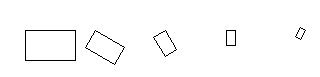
\includegraphics[width=0.75\textwidth]{../img/turtle/RectSeq.png}
%\caption Rotation av rektangel med koden nedan.
%\label{fig:classes:graphics:rollingrectangle}
\end{figure}
\noindent Bilden ovan kan skapas med hjälp av denna kod:
\begin{Code}
  def rectSeqExample(t: Turtle): Unit  = {
    val rect = Rect(pos = Point(200, 200), width = 50, height = 30)
    RectSeq(rect, n = 5, dist = 70, rot = -30, scale = 0.67).draw(t)
  }
\end{Code}

\noindent Nedan kod ritar bilden i fig. \ref{fig:classes:graphics:rectanglesequence} på sidan \pageref{fig:classes:graphics:rectanglesequence}. Använd gärna \code{setLineColor} i \code{SimpleWindow} för att göra en färggladare stjärna. Slumpvisa transformationer är också kul. 

\begin{Code}
val w = new SimpleWindow(500, 500, "Shapes")
val t = new Turtle(w, new Point(200, 200), 0, false)
val rect = Rect(pos = Point(225, 235), width = 50, height = 30)
val roll = RectSeq(rect, n = 100, dist = 2, scale = 0.98)
for (i <- 0 to 360 by 20) roll.rotatedLeft(i).draw(t)
\end{Code}


\begin{figure}
\centering
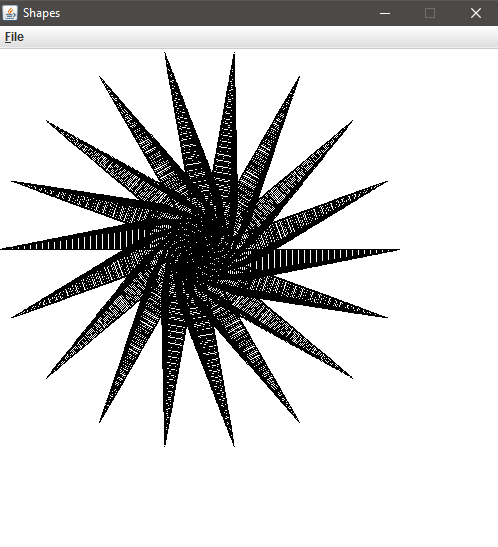
\includegraphics[width=0.5\textwidth]{../img/w06-lab/RectangleSequence.png}
\caption {En stjärna skapad med hjälp av \code{RectSeq}.}
\label{fig:classes:graphics:rectanglesequence}
\end{figure}

\noindent Nedan finns ett kodskellett som du kan utgå ifrån. Dokummentationskommentarerna innehåller fler detaljer om hur det är tänkt att klassen ska fungera. %De metoder som returnerar \code{RectSeq} ska returnera en referens till den egna instansen så att upprepad punktnotation möjliggörs.

\begin{figure}[H]
\scalainputlisting[numbers=left,basicstyle=\ttfamily\fontsize{9.9}{12}\selectfont]%
{../workspace/w05_turtle/src/main/scala/graphics/RectSeq.scala}
\label{code:classes:graphics:rectanglesequence}
\end{figure}



%\Task En riktig utmaning, för den som har lust: Implementera spelet ''Masken'' som beskrivs här: \url{https://sv.wikipedia.org/wiki/Snake}.


%%!TEX encoding = UTF-8 Unicode
\chapter{Sekvenser}\label{chapter:W06}
Begrepp som ingår i denna veckas studier:
\begin{multicols}{2}\begin{itemize}[noitemsep,label={$\square$},leftmargin=*]
\item översikt av Scalas samlingsbibliotek och samlingsmetoder
\item klasshierarkin i scala.collection
\item Traversable
\item Iterable
\item Seq
\item List
\item ListBuffer
\item ArrayBuffer
\item WrappedArray
\item sekvensalgoritm
\item algoritm: SEQ-COPY
\item in-place vs copy
\item algoritm: SEQ-REVERSE
\item registrering
\item algoritm: SEQ-REGISTER
\item linjärsökning
\item algoritm: LINEAR-SEARCH
\item tidskomplexitet
\item minneskomplexitet
\item sekvenser i Java vs Scala
\item for-sats i Java
\item java.util.Scanner
\item översikt strängmetoder
\item StringBuilder
\item ordning
\item inbyggda sökmetoder
\item find
\item indexOf
\item indexWhere
\item inbyggda sorteringsmetoder
\item sorted
\item sortWith
\item sortBy
\item variabelt argumentantal\end{itemize}\end{multicols}

%!TEX encoding = UTF-8 Unicode

%!TEX root = ../compendium1.tex

\Lab{\LabWeekSIX}

\begin{Goals}
%\item Kunna skapa en klass utifrån en textuell beskrivning. % av dess medlemmar.
%\item Kunna skapa en klass utifrån ofärdig kod och dokumentationskommentarer.
%\item Kunna införa privata attribut med lämpliga namn som representerar instansers förändringsbara tillstånd.
\item Kunna förklara skillnader och likheter mellan ett singelobjekt och objekt som är instanser av klasser.
\item Kunna förklara skillnaden mellan förändringsbara och oföränderliga objekt.
\item Kunna definiera och instansiera klasser och case-klasser, samt kunna beskriva när en case-klass är lämpligast och ge några exempel på vad en sådan erbjuder utöver en vanlig klass.
\item Kunna skapa och använda klasser vars instanser innehåller referenser till andra instanser (aggregering).
\item Förstå innebörden av instansreferensen \code{this}.
\item Kunna skapa enkla match-uttryck.
\end{Goals}

\begin{Preparations}
\item \DoExercise{\ExeWeekFIVE}{05}, speciellt uppgift \ref{exe:classes:labprep}.
\item \DoExercise{\ExeWeekSIX}{06}.
\item Läs igenom hela laborationen och planera ditt arbete.
\item Hämta given kod via \href{https://github.com/lunduniversity/introprog/tree/master/workspace/}{kursen github-plats} eller via hemsidan under \href{https://cs.lth.se/pgk/download/}{Download}.

\end{Preparations}

\subsection{Bakgrund}

{\raggedright%
\begin{minipage}{0.42\textwidth}
\begin{figure}[H]
  %\centering
  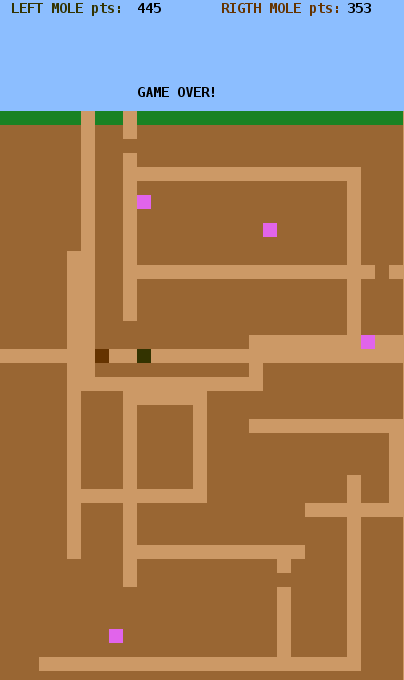
\includegraphics[width=1.0\textwidth]{../img/blockbattle.png}
  \caption{En duell om blockmaskar mellan två lundensiska blockmullvader fångade på bild under intensivt grävanade.}
  \label{lab:blockbattle:fig:game}
\end{figure}
\end{minipage}%
}%
\newlength{\currentparskip}%
\newlength{\currentparindent}%
{
\setlength{\currentparskip}{\parskip}% save the value
\setlength{\currentparindent}{\parindent}% save the value
\hfill%
\begin{minipage}{0.47\textwidth}
\setlength{\parskip}{\currentparskip}% restore the value
\setlength{\parindent}{\currentparindent}% restore the value
\noindent Under denna laboration ska du träna på att deklarera klasser och skapa flera instanser av samma klass. Du tränar även på att bygga ett större program från grunden.

Du ska utveckla ett spel för två spelare som sitter vid samma tangentbord, där den vänstra spelaren styr en blockmullvad med tangenterna A,S,D,W, och den högra spelaren styr en annan blockmullvad med piltangenterna.

I bilden till vänster ser du hur spelet kan se ut. Det finns en ljusbrun och en mörkbrun mullvad. Poängräkningen visas överst i himlen. Det finns fyra rosa blockmaskar (se uppgift \ref{lab:blockmole:task:blockworm} i laboration \code{blockmole}) som mullvadarna tävlar om att försöka fånga. När en blockmask teleporterar sig till en ny slumpmässig position lämnar den jord efter sig. När en mullvad gräver sig upp till gräsytan blir det hål i gräset.
Det ger poäng att gräva tunnlar och att fånga blockmaskar.

Du bestämmer själv hur poängsättningen ska ske och kriteriet för när spelet är slut etc.
\end{minipage}%
}



\subsection{Obligatoriska krav}

Följande funktionella krav ska uppfyllas av ditt program:
\begin{itemize}[nosep, label={$\square$},]
%\item Det ska finnas två blockmullvadar, en för vänster spelare och en för höger spelare, som styrs med ASDW resp. piltangerna.
\item Varje mullvad rör sig i sin aktuella riktning tills användaren ändrar riktning genom att trycka på ''sin'' motsvarande knapp, t.ex. W eller pil-upp.
\item Då en mullvad går i mörkbrun jord ska ljusbruna tunnlar grävas.
\item Då en blockmullvad når fönstrets kant eller himlen ska dess riktning reverseras.
\item Det ska ge poäng att gräva tunnlar.
\item Varje spelares poäng ska visas under spelets gång.
\item Ett spel ska avslutas och \emph{Game over} visas när något valfritt kriterium uppfyllts.
%\item Vid \emph{Game over} ska man kunna välja att avsluta programmet eller spela igen.
\end{itemize}

\noindent Din kod ska utformas enligt dessa design-krav:
\begin{itemize}[nosep, label={$\square$}]
\item Ett \code{Game} skapas i huvudprogrammet med metoden \code{start} som kör igång spelet.
\item Konstanter ska namnges och placeras i lämpligt kompanjonsobjekt.
\item Varje klass med ev. tillhörande kompanjonsobjekt ska finnas i en egen kodfil och tillhöra paketet \code{blockbattle}.
\item Du ska utgå från klasserna som du implementerat i uppgift \ref{exe:classes:labprep} i övning \texttt{\ExeWeekFIVE}.
\item Klassen \code{BlockWindow} omvandlar till interna fönsterkoordinater. Övriga klasser ska använda block-koordinater.
\end{itemize}


\subsection{Valbara krav -- välj minst ett}

Du ska implementera minst ett (gärna flera) av dessa krav:
\begin{itemize}[nosep, label={$\square$}]
\item Det ska finnas lagom många blockmaskar (se labb \code{blockmole} uppg. \ref{lab:blockmole:task:blockworm},  sid. \pageref{lab:blockmole:task:blockworm}).
\item Blockmullvadarna ska även ha ett attribut som representerar hälsan, t.ex. ett numeriskt värde mellan 0 och 100. Hälsan ska försvagas något när man gräver tunnlar. Hälsan ska synas i spelfönstret, t.ex. som en sekvens med röda block i himlen som indikerar andelen av maxhälsan för resp. spelare.
\item Att springa på gräset ska påverka poäng och/eller hälsa.
\item Att fånga blockmask ska påverka poäng och/eller hälsa.
\item Det ska finnas gula blockdiamanter som ger många poäng om man tar dem först.
\item Det ska vid spelstart gå att välja namn på respektive blockmullvad och namnet ska synas i spelet vid poängutskriften.
\item Det ska gå fortare att gå i gångar jämfört med att gräva i jord.
\item Om en blockmullvad fångar en blockmask ska dess grävhastighet öka.
\item Om en blockmullvad krockar med en annan blockmullvad ska något hända, t.ex. att dess riktning reverseras.
\item Visa \emph{highscore} vid \emph{Game Over}.  Highscore sparas med \code{introprog.IO} i en fil som skapas om den inte finns annars läses in vid uppstart om den finns och uppdateras vid behov. Spara hela highscore-listan eller bara högsta poäng hittills.
\end{itemize}

\subsection{Förebredelser inför redovisningen}
\Checkpoint\noindent Innan du redovisar din implementation ska du muntligt kunna redogöra för följande:
\begin{itemize}[nosep, label={$\square$}]
  \item Studera någon annans spel och ge din kamrat minst ett tips om hur kodens läsbarhet kan förbättras. Skriv ner dina tips och beskriv dem vid redovisningen.
  \item Beskriv vilka åtgärder du gjort för att din kod ska vara lätt att läsa och förstå.
  \item Beskriv hur du stegvis utvecklat ditt program från enklare till mer avancerad funktionalitet, samt vilka buggar du upptäckt och fixat.
  \item Beskriv vilket eller vilka valfria krav som din implementation uppfyller.
  \item Beskriv hur du hade behövt ändra i klassen \code{Mole} för att det ska gå att skriva\\\code{new Mole().move().move().reverseDir().move()}
\end{itemize}

\subsection{Tips och förslag}

\begin{enumerate}[leftmargin=*]
  \item \textbf{Många små steg.} Kör kompilering under ändringsbevakning med \code{--watch} i ett eget terminalfönster, så att du vid varje ändring kan rätta ev. kompileringsfel. Kör och testa ditt program ett annat terminalfönster.

  \item \textbf{Inför bra namn}. Din kod blir lättare att läsa och ändra i om du hittar på bra namn på medlemmar och lägger dem på lämpligt ställe. T.ex. kan du samla globala spel-konstanter i kompanjonsobjektet till klassen \code{Game}. Du kan bygga vidare på nedan kod och lägga till medlemmar allteftersom du upptäcker att de behövs. Nedan finns exempelvis en funktion som ger bakgrundsfärgen för en viss y-koordinat, vilken är användbar när du ska återställa bakgrunden efter att en mullvad har flyttat sig.
\scalainputlisting[basicstyle=\ttfamily\fontsize{10}{12}\selectfont]{../workspace/w06_blockbattle/Game.scala}
% \begin{CodeSmall}
% object Game {
%   val windowSize = (30, 50)
%   val windowTitle = "EPIC BLOCK BATTLE"
%   val blockSize = 14
%   val skyRange    = 0 to 7
%   val grassRange  = 8 to 8
%   object Color { ??? }
%   def backgroundColorAtDepth(y: Int): java.awt.Color = ???
% }
%
% class Game(
%   val leftPlayerName: String  = "LEFT",
%   val rightPlayerName: String = "RIGHT"
% ) {
%  import Game.* // direkt tillgång till namn på medlemmar i kompanjon
%
%  val window    = new BlockWindow(windowSize, windowTitle, blockSize)
%  val leftMole  = ???
%  val rightMole = ???
%
%  def drawWorld(): Unit = ???
%
%  def eraseBlocks(x1: Int, y1: Int, x2: Int, y2: Int): Unit = ???
%
%  def update(mole: Mole): Unit = ???  // update, draw new, erase old
%
%  def gameLoop(): Unit = ???
%
%  def start(): Unit = {
%    println("Start digging!")
%    println(s"$leftPlayerName ${leftMole.keyControl}")
%    println(s"$rightPlayerName ${rightMole.keyControl}")
%    drawWorld()
%    gameLoop()
%  }
% }
% \end{CodeSmall}

 \item \textbf{Dela upp din kod i funktioner.} Din kod blir lättare att läsa och ändra i om du delar upp den i många små funktioner med bra namn. I \code{Game}-klassen ovan finns exempel på några användbara funktioner. Allteftersom du utvidgar ditt program kan du lägga till fler funktioner som t.ex. heter \code{showPoints}, \code{gameOver}, etc.

\item \textbf{Tänk igenom den övergripande strukturen.} Programmet du ska skriva i denna laboration är större än det du gjort tidigare. Det är därför viktigt att tänka igenom strukturen på ditt program, vilka klasser som har hand om vad och hur de samarbetar. Diskutera gärna med handledare om du är osäker på hur de koddelar du utvecklat i föregående veckas övning \ref{exe:classes:labprep}, klasserna \code{Pos}, \code{KeyControl}, \code{Mole} och \code{BlockWindow}, är tänkt at samverka. Var noga med att testa så de olika klasserna och deras metoder fungerar var för sig.     

\item \textbf{Utformning av \texttt{gameLoop()}}. I ett spel behövs en s.k. spel-loop \Eng{game loop} som upprepar den kod som ska köras vid varje ny skärmbild, ofta kallad \emph{frame}. I varje runda i spel-loopen sker uppdatering av data och ritning i spelfönstret, samt en lämplig fördröjning. En skiss på en typisk spel-loop visas nedan:
\begin{CodeSmall}
  var quit = false
  val delayMillis = 80

  def gameLoop(): Unit = 
    while !quit do
      val t0 = System.currentTimeMillis
      handleEvents()    // ändrar riktning vid tangenttryck etc.
      update(leftMole)  // flyttar, ritar, suddar, etc.
      update(rightMole)

      val elapsedMillis = (System.currentTimeMillis - t0).toInt
      Thread.sleep((delayMillis - elapsedMillis) max 0)
    end while
  end gameLoop
\end{CodeSmall}

\item \textbf{Hantering av händelser.} Ett \code{BlockWindow}, som du implementerade i uppgift \ref{exe:classes:labprep} i övning \texttt{\ExeWeekFIVE}, kan via anrop av \code{nextEvent} ge   \code{KeyPressed(key)} vid knapptryck och \code{WindowClosed} vid fönsterstängning. Om ingen händelse finns att behandla returneras \code{Undefined}. Använd en loop som betar av alla händelser tills \code{Undefined} påträffas, enligt nedan:

\begin{CodeSmall}
  def handleEvents(): Unit = 
    var e = window.nextEvent()
    while e != BlockWindow.Event.Undefined do
      e match 
        case BlockWindow.Event.KeyPressed(key) =>
          ???  // ändra riktning på resp. mullvad

        case BlockWindow.Event.WindowClosed =>
          ???  // avsluta spel-loopen
      
      e = window.nextEvent()
    end while
  end handleEvent
\end{CodeSmall}

\item \textbf{Flimmerfri grafik.} För att minska mängden flimmer \Eng{flicker} är det bäst att i varje iteration i spel-loopen (1) bara rita om det som ändrats för att minimera tiden som spenderas på att rita, och (2) vid ändringar rita nya delar före att gamla delar raderas. För att slippa mullvadsflimmer kan du ''\emph{rita först -- sudda sen}'' enligt nedan.\footnote{Inom spelutveckling använder man oftast istället så kallad \emph{double buffering} (eller till och med \emph{triple buffering}) för att få helt flimmerfri grafik. Det ligger dock bortom kursen och stöds inte av \code{PixelWindow}.}

% \begin{CodeSmall}
% val oldMolePos = mole.pos                  // save
% mole.move()                                // update
% window.setBlock(mole.pos, mole.color)      // draw new
% window.setBlock(oldMolePos, Color.tunnel)  // erase old
% \end{CodeSmall}

\begin{CodeSmall}
window.setBlock(mole.nextPos, mole.color) // draw new
window.setBlock(mole.pos, Color.tunnel)   // erase old
mole.move()                               // update
\end{CodeSmall}

\end{enumerate}


%\chapter{Arv, Gränssnitt}
\begin{itemize}[nosep]
\item klasser
\item arv
\item polymorfism
\item likhet
\item equals
\item accessregler
\item private
\item public
\item protected
\item private[this]
\item trait
\item inmixning
\item Any
\item AnyVal
\item AnyRef
\item Nothing\end{itemize}
%!TEX encoding = UTF-8 Unicode

%!TEX root = ../compendium1.tex

\Lab{\LabWeekSEVEN}

\begin{Goals}
%!TEX encoding = UTF-8 Unicode
%!TEX root = ../compendium1.tex

\item Kunna skapa och använda sekvenssamlingar.
\item Kunna implementera sekvensalgoritmen SHUFFLE som modifierar innehållet i en array på plats.
\item Kunna registrera antalet förekomster av olika värden i en sekvens.

\end{Goals}

\begin{Preparations}
\item \DoExercise{\ExeWeekSEVEN}{07}
\item Läs igenom hela laborationen och säkerställ att du förstår hur SHUFFLE-algoritmen nedan fungerar.

\item Studera den givna koden i kursens workspace på GitHub här:\\
\url{https://github.com/lunduniversity/introprog/tree/master/workspace}

\end{Preparations}

\subsection{Bakgrund}\label{knuth-shuffle}

Denna uppgift handlar om kortblandning. Att blanda kort så att varje möjlig permutation (ordning som korten ligger i) är lika sannolik är icke-trivialt; en osystematisk blandning leder till en skev fördelning.

Givet en bra slumpgenerator går det att blanda en kortlek genom att lägga alla kort i en hög och sedan ta ett slumpvist kort från högen och lägga det överst i leken, tills alla kort ligger i leken. Fisher-Yates-algoritmen\footnote{\href{https://en.wikipedia.org/wiki/Fisher\%E2\%80\%93Yates_shuffle}{https://en.wikipedia.org/wiki/Fisher\%E2\%80\%93Yates\_shuffle}} (även kallad Knuth-shuffle), fungerar på det sättet. Här benämner vi denna algoritm SHUFFLE. Den återfinns i pseudokod nedan:

\begin{algorithm}[H]
 \SetKwInOut{Input}{Indata}
 \SetKwInOut{Output}{Utdata}
 \Input{Array $xs$ med $n$ st värden som ska blandas ''på plats''}
 \Output{$xs$ med sina värden omflyttade i slumpmässig ordning}
 \For{$i \leftarrow (n - 1)$ \KwTo $0$}{
  $r \leftarrow$ slumptal mellan $0$ och $i$ \\
  byt plats på $xs(i)$ och $xs(r)$
%  $temp \leftarrow xs(i)$ \\
%  $xs(i) \leftarrow xs(r)$ \\
%  $xs(r) \leftarrow temp$ \\
 }
\end{algorithm}

En kortlek \Eng{deck} har 52 kort, vart och ett med olika valör \Eng{rank} och färg (eng. \emph{suit}, på svenska även svit). Kortspelet poker handlar om att dra kort och få upp vissa kombinationer av kort, s.k. ''händer''\footnote{\href{https://sv.wikipedia.org/wiki/Pokerhand}{https://sv.wikipedia.org/wiki/Pokerhand}}. Dessa är ordnade från bättre till sämre; den spelare som får bäst hand vinner.
Det är därför intressant att veta med vilken sannolikhet en viss hand dyker upp vid dragning från en blandad kortlek.

De vanliga pokerhänderna är, i fallande värde, färgstege (straight flush), fyrtal, kåk (full house), färg (flush), stege (straight), triss, tvåpar och par. Dessa finns illustrerade i avsnitt \ref{shuffle:hands}.
Det finns ytterligare en hand, s.k. ''royal (straight) flush'' som betecknar en färgstege med ess som högsta kort, men dess sannolikhet är för låg för att man vid simulering kan förväntas påträffa den inom rimlig tid.

Under laborationen ska du börja med att göra klar den ofärdiga klassen \code{Deck} som visas nedan, och återfinns i workspace på GitHub.



Labbinstruktionerna i avsnitt \ref{subsection:lab:shuffle:tasks} ger tips om hur du ska ersätta \code{???} i givna kodskelett med med dina lösningar.
Med hjälp av klasserna \code{TestHand} och \code{TestDeck} kan du testa så att dina implementationer fungerar.

\begin{figure}
\scalainputlisting[numbers=left,basicstyle=\ttfamily\fontsize{10}{12}\selectfont]{../workspace/w07_shuffle/src/main/scala/cards/Card.scala}
\caption{Den färdigimplementerade, oföränderliga case-klassen \code{Card}.}
\label{shuffle:fig-card}
\end{figure}




När dina implementationer av metoderna \code{full} och \code{shuffle} fungerar ska du använda \code{Deck} i singelobjektet \code{PokerProbability} för att ta reda på sannolikheter för att olika pokerhänder uppkommer när man delar ut 5 kort ur en bra blandad kortlek.

Till din hjälp har du nedan kodfiler, där några har ofärdig kod som du ska färdigställa. All kod  ligger i ett paket med namnet \code{cards}.\footnote{Du kan bläddra bland klasserna i paketet cards här: \\
\href{https://github.com/lunduniversity/introprog/tree/master/workspace/w07_shuffle/src/main/scala/cards}{\mbox{\fontsize{9}{11}\selectfont  https://github.com/lunduniversity/introprog/tree/master/workspace/w07\_shuffle/src/main/scala/cards}}}

\begin{itemize}
\item \code{Card.scala} i fig. \ref{shuffle:fig-card} innehåller den färdigimplementerade case-klassen \code{Card} som representerar ett kort och har en koncis \code{toString} med valör och svit (färg).

\item \code{Deck.scala} i fig. \ref{shuffle:fig-deck} innehåller den förändringsbara klassen \code{Deck}, där du ska implementera kortblandning i metoden \code{shuffle}. Kompanjonsobjektet har metoder för att skapa kortlekar. Du ska implementera metoden \code{full} som skapar en fullständig kortlek med de 52 korten ordnade efter valör och färg.

\item \code{Hand.scala} i fig. \ref{shuffle:fig-hand} innehåller en case-klass \code{Hand} som representerar en pokerhand och har metoder för att avgöra vilken hand det är. I kompanjonsobjektet finns fabriksmetoder som kan skapa en ny hand från enskilda kort eller genom att dra kort ur en kortlek. Du ska implementera \code{tally} som registrerar antalet kort av en viss valör.

\item \code{PokerProbability.scala} i fig. \ref{shuffle:fig-pokerprob}  har en main-metod som räknar ut pokersannolikheter, samt hjälpmetoden \code{register} som du ska implementera.

\item \code{TestDeck.scala} ska du använda för att testa din implementation av \code{shuffle} med en kortlek som endast innehåller tre kort. Upprepade blandningar görs och förekomsten av varje möjlig permutation  registreras.

\item \code{TestHand.scala} har en \code{main}-metod som testar klassen \code{Hand}.

%\item \code{AsciiBarGraph.scala} innehåller enbart en metod som skapar ett stapeldiagram åt \code{TestingDeck}
\end{itemize}

\begin{figure}
\scalainputlisting[numbers=left,basicstyle=\ttfamily\fontsize{10}{12}\selectfont]{../workspace/w07_shuffle/src/main/scala/cards/Deck.scala}
\caption{Den ofärdiga klassen \code{Deck} med förändringsbar kortlek.}
\label{shuffle:fig-deck}
\end{figure}



\begin{figure}
\scalainputlisting[numbers=left,basicstyle=\ttfamily\fontsize{9}{10.5}\selectfont]{../workspace/w07_shuffle/src/main/scala/cards/Hand.scala}
\caption{Den ofärdiga, oföränderliga klassen \code{Hand} som representerar en pokerhand.}
\label{shuffle:fig-hand}
\end{figure}

\begin{figure}
\scalainputlisting[numbers=left,basicstyle=\ttfamily\fontsize{10}{12}\selectfont]{../workspace/w07_shuffle/src/main/scala/cards/PokerProbability.scala}
\caption{Det ofärdiga singelobjektet \code{PokerProbability} som tar reda på sannolikheter för olika pokerhänder.}
\label{shuffle:fig-pokerprob}
\end{figure}


\subsection{Obligatoriska uppgifter}\label{subsection:lab:shuffle:tasks}


\Task Implementera algoritmen SHUFFLE.

\Subtask Skapa din egen implementation av metoden \code{shuffle} i klassen \code{Deck}. Följ den givna algoritmen i stycke \ref{knuth-shuffle} noga. Du kan använd \code{cards.length} för att få fram längden på kortleken, men du kan gärna istället använda \code{cards.indices.reverse}. Implementera och använd metoden  \code{swap}.

\Subtask Kör \code{testShuffle} i \code{TestDeck} som kontrollerar att blandningen är jämnt fördelad genom att blanda en kortlek med tre kort och räkna hur ofta varje möjlig permutation dyker upp. Du bör få en utskrift med sex ($3!$) procentsatser som ska vara nästan lika.


\Task Skapa en fullständig, ordnad kortlek.

\Subtask Implementera metoden \code{full} som skapar en 52-korts standardlek ordnad efter färg och valör. Använd \code{Range}-värdena i kompanjonsobjektet \code{Card}.

\Subtask Kör \code{testCreate} i \code{TestDeck} och kontrollera så att du får kort av alla fyra färger, samt både ess och kungar.


\Task Gör färdigt och testa \code{Hand}.

\Subtask Implementera \code{tally} som ska ge en indexerbar sekvens med 14 platser där plats 1-13 innehåller antalet av respektive valör. (Plats 0 ska inte användas.)

\Subtask Testa klassen \code{Hand} med hjälp av \code{TestHand}.


\Task Ta fram sannolikheterna för ''straight flush'', ''straight'' och ''flush''.

\Subtask Implementera metoden \code{register} i \code{PokerProbability}. Använd \code{from} och \code{category} i \code{Hand} för att skapa och kategorisera en hand från en kortlek. Lagra frekvenserna i en lokal array som du, när resultatet är färdigt, gör om till en vektor med \code{toVector}.

\Subtask Kör \code{PokerProbability}, förslagsvis med en miljon iterationer. Du bör få ungefär dessa sannolikheter\footnote{\url{http://www.forum.gpcdata.se/pdf/poker.pdf}}:
\begin{figure}[H]\centering
\begin{tabular}{r|l}
\emph{hand} & $\emph{sannolikhet}$ \\ \hline
Straight flush & 0.00154\%  \\
Flush          & 0.197\%    \\
Straight       & 0.39\%     \\
\end{tabular}
\end{figure}

\Task Kopiera hela din lösning till en ny katalog och ändra implementationen så att du drar nytta av uppräknade datatyper med \code{enum} i stället för heltal och strängsekvenser. Diskutera med handledare för- och nackdelar med de två olika implementationerna. 

\subsection{Frivilliga extrauppgifter}


\Task Förbättra programmet så att simuleringen registrerar alla handkategorier utom Royal Flush. Kör sedan \code{PokerProbability} igen och notera sannolikheterna.

\Task Gör om alla metoder i case-klassen \code{Hand} till \code{lazy val} och undersök hur det påverkar exekveringstiden. Varför förändras prestanda med denna åtgärd? Hade denna optimering varit lämplig om klassen \code{Hand} vore förändringsbar? Varför?

\Task Gör så att även sannolikheten för Royal Flush kan simuleras. Det krävs i storleksordningen $10^8$ iterationer för en noggrannhet på 2 värdesiffror. Detta kan ta ca 5 minuter på en någorlunda snabb dator, så det kan vara läge före en paus under simuleringen...

\Task Implementera ett interaktivt kortspel, t.ex. någon enkel pokervariant. Börja med något mycket enkelt, till exempel högst-kort-vinner, och bygg vidare med sådant som du tycker verkar roligt.

Du kan t.ex. skapa en metod \code{def compareTo(other: Hand): Comparison} i case-klassen \code{Hand} som ger \code{Comparison.Worse} om \code{other} är sämre, \code{Comparison.Equal} om händerna är lika bra, och \code{Comparison.Better} om \code{other} är bättre. Du kan steg för steg göra så att det går att jämföra fler och fler händer enligt de specialregler som gäller för när olika händer anses bättre eller lika. Läs om reglerna här: \url{https://en.wikipedia.org/wiki/List_of_poker_hands}



\subsection{Bilder med exempel på olika pokerhänder}\label{shuffle:hands}

Figurerna \ref{lab:shuffle:first-picture} -- \ref{lab:shuffle:last-picture} visar bilder på olika korthänder i poker.

\newcommand{\CardWidth}{0.5\textwidth}
\newcommand{\CardCaptionWidth}{0.3\textwidth}

\begin{figure}[H]
 \begin{minipage}[c]{\CardWidth}
  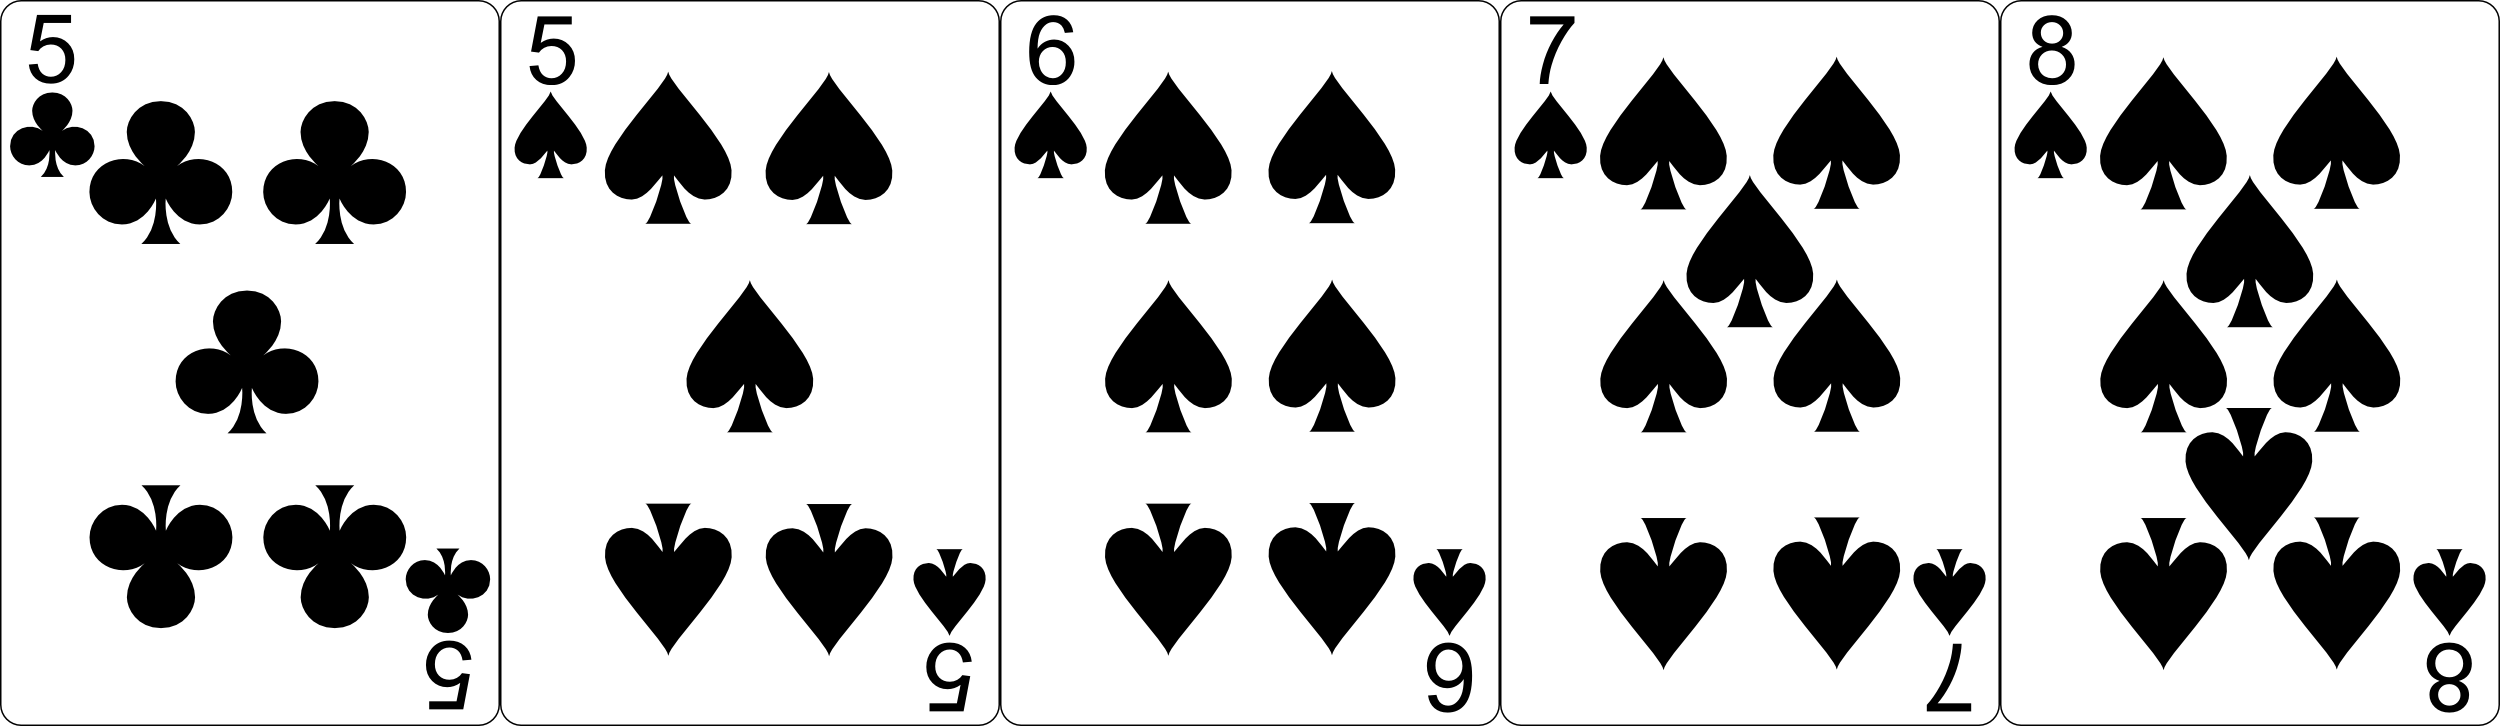
\includegraphics[width=\textwidth]{../img/w05-hands/pair.png}
 \end{minipage}
 \begin{minipage}[c]{\CardCaptionWidth}
  \caption{Par: två kort har samma valör.}
   \label{lab:shuffle:first-picture}
 \end{minipage}
\end{figure}

\begin{figure}[H]
 \begin{minipage}[c]{\CardWidth}
  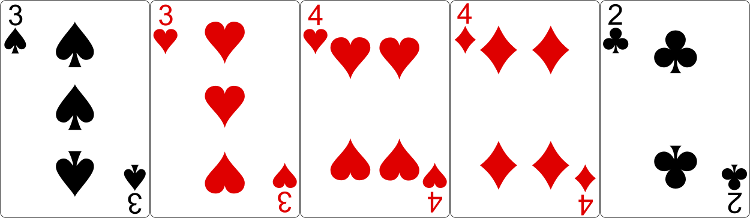
\includegraphics[width=\textwidth]{../img/w05-hands/twopair.png}
 \end{minipage}
 \begin{minipage}[c]{\CardCaptionWidth}
  \caption{Två par: handen har två \emph{olika} par.}
 \end{minipage}
\end{figure}

\begin{figure}[H]
 \begin{minipage}[c]{\CardWidth}
  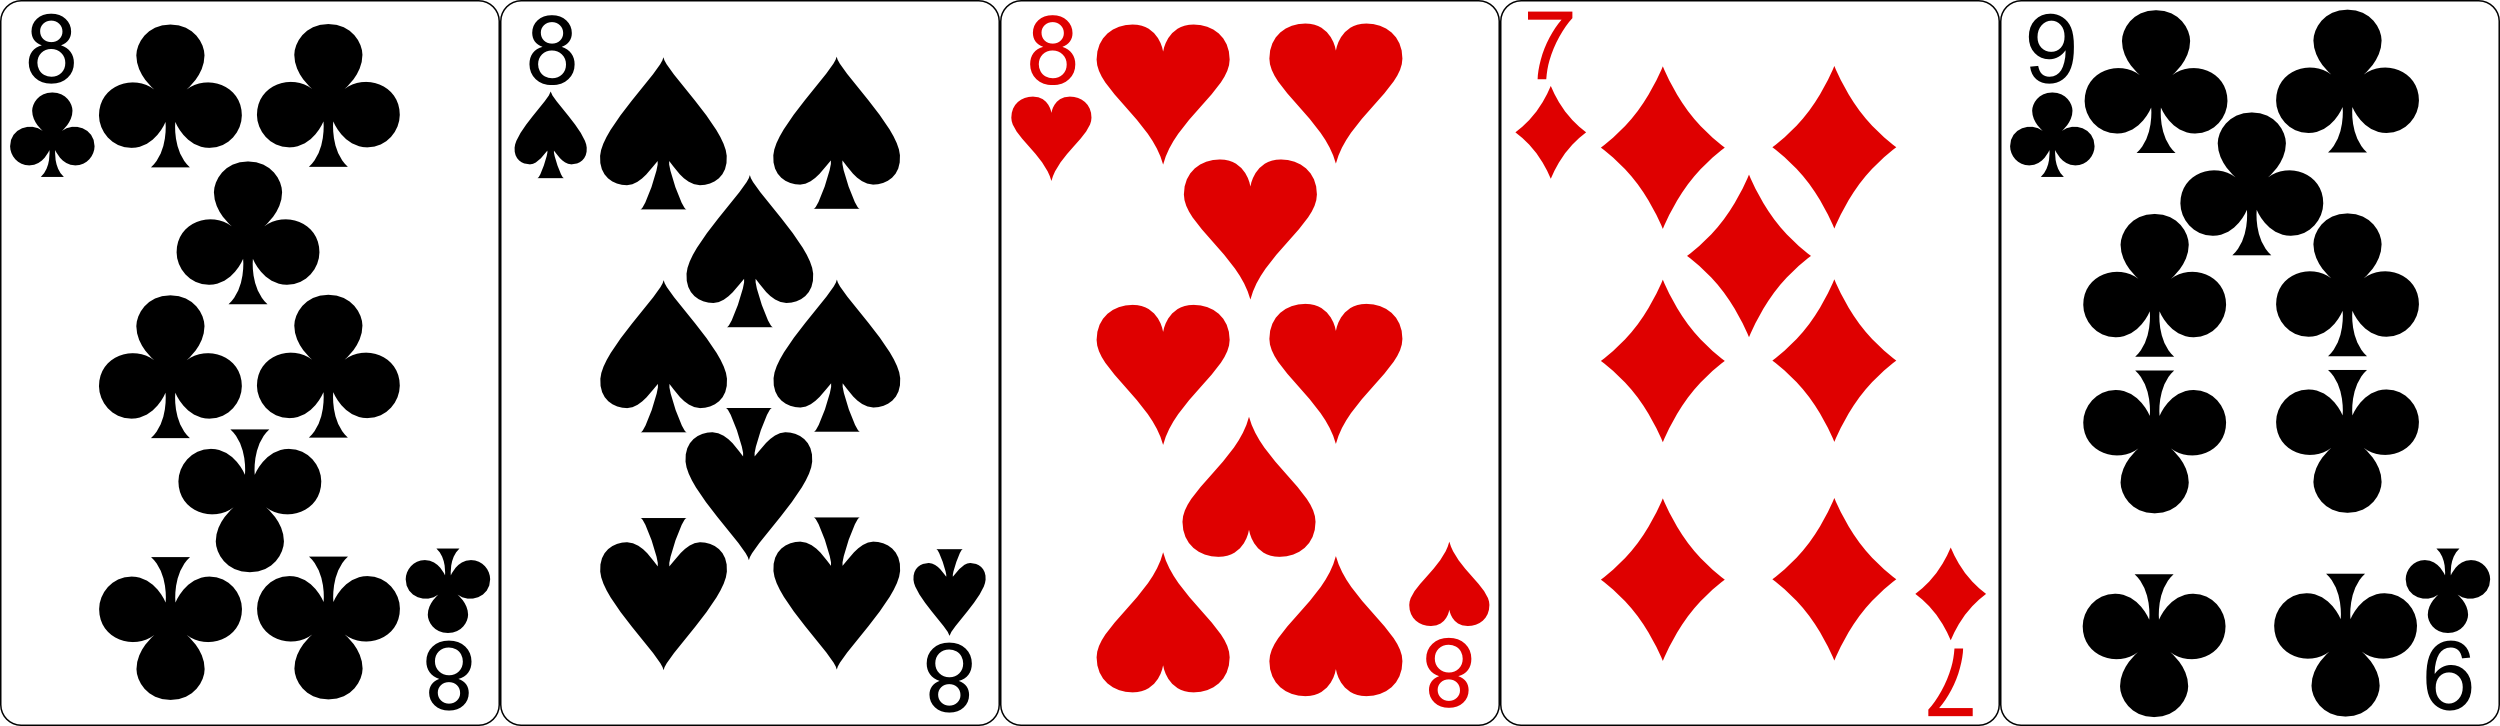
\includegraphics[width=\textwidth]{../img/w05-hands/trips.png}
 \end{minipage}
 \begin{minipage}[c]{\CardCaptionWidth}
  \caption{Triss: tre kort har samma valör.}
 \end{minipage}
\end{figure}

\begin{figure}[H]
 \begin{minipage}[c]{\CardWidth}
  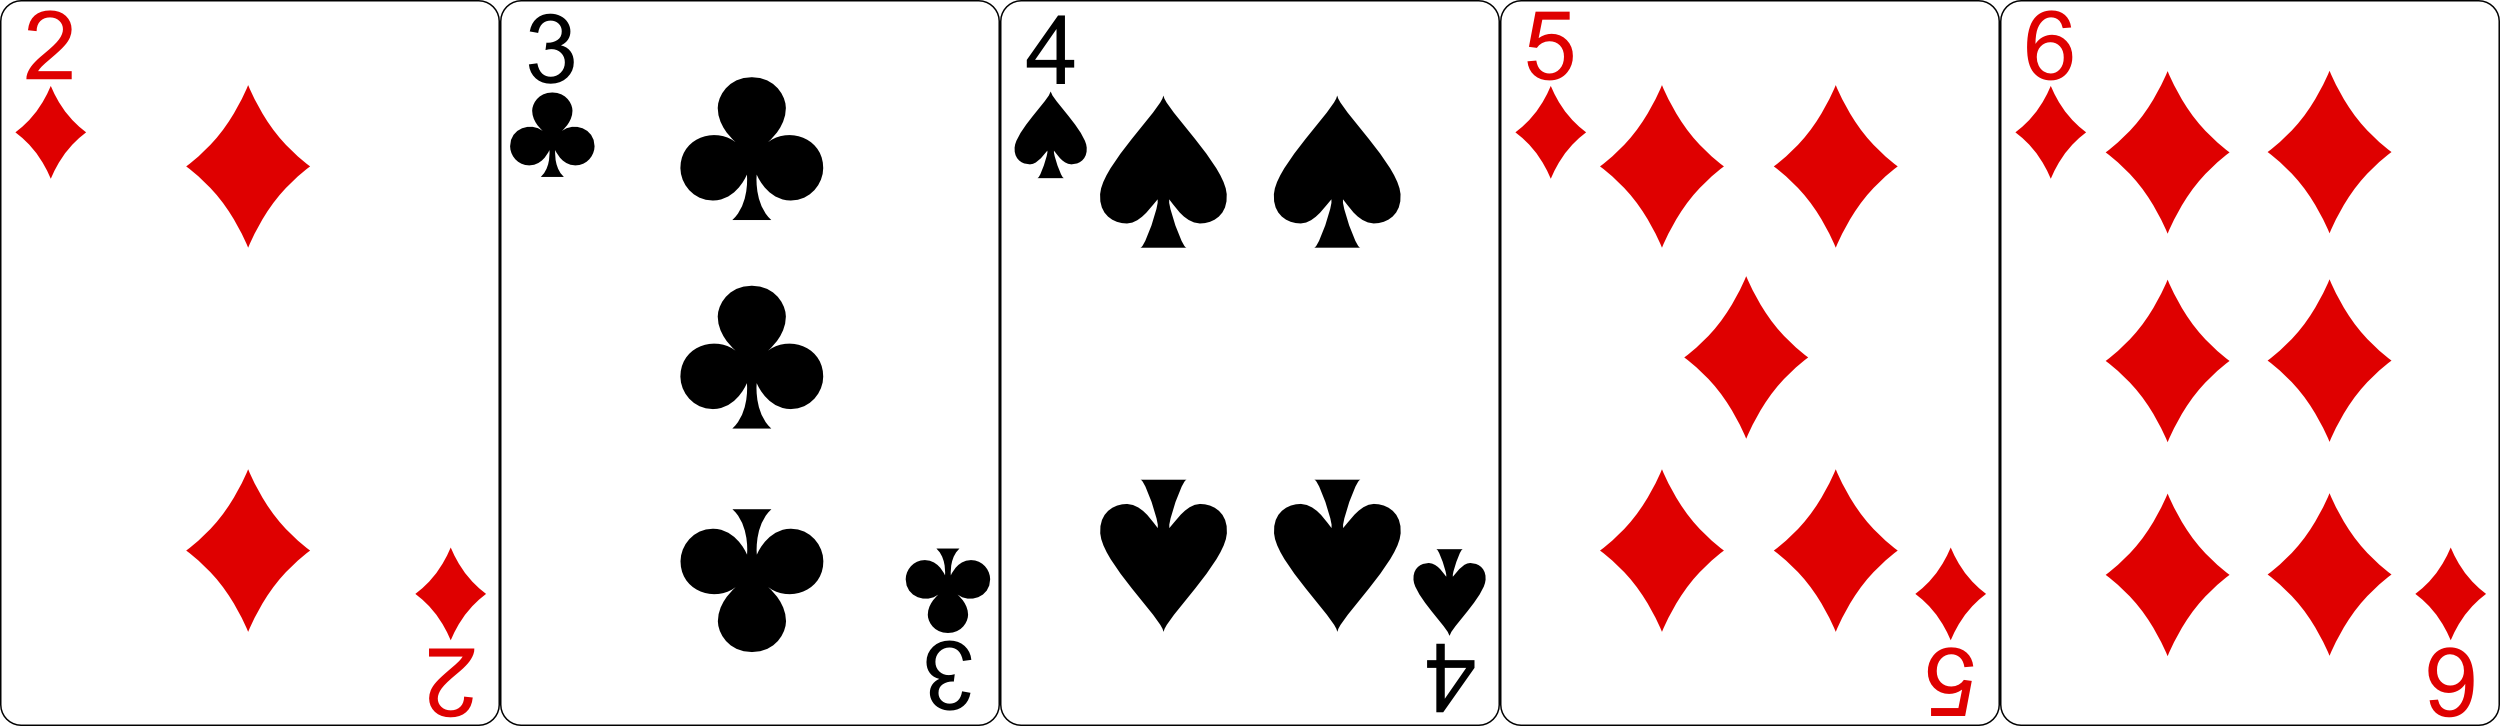
\includegraphics[width=\textwidth]{../img/w05-hands/straight.png}
 \end{minipage}
 \begin{minipage}[c]{\CardCaptionWidth}
  \caption{Stege: kortens valörer bildar en följd, ess kan vara antingen 1 eller 14.}
 \end{minipage}
\end{figure}

\begin{figure}[H]
 \begin{minipage}[c]{\CardWidth}
  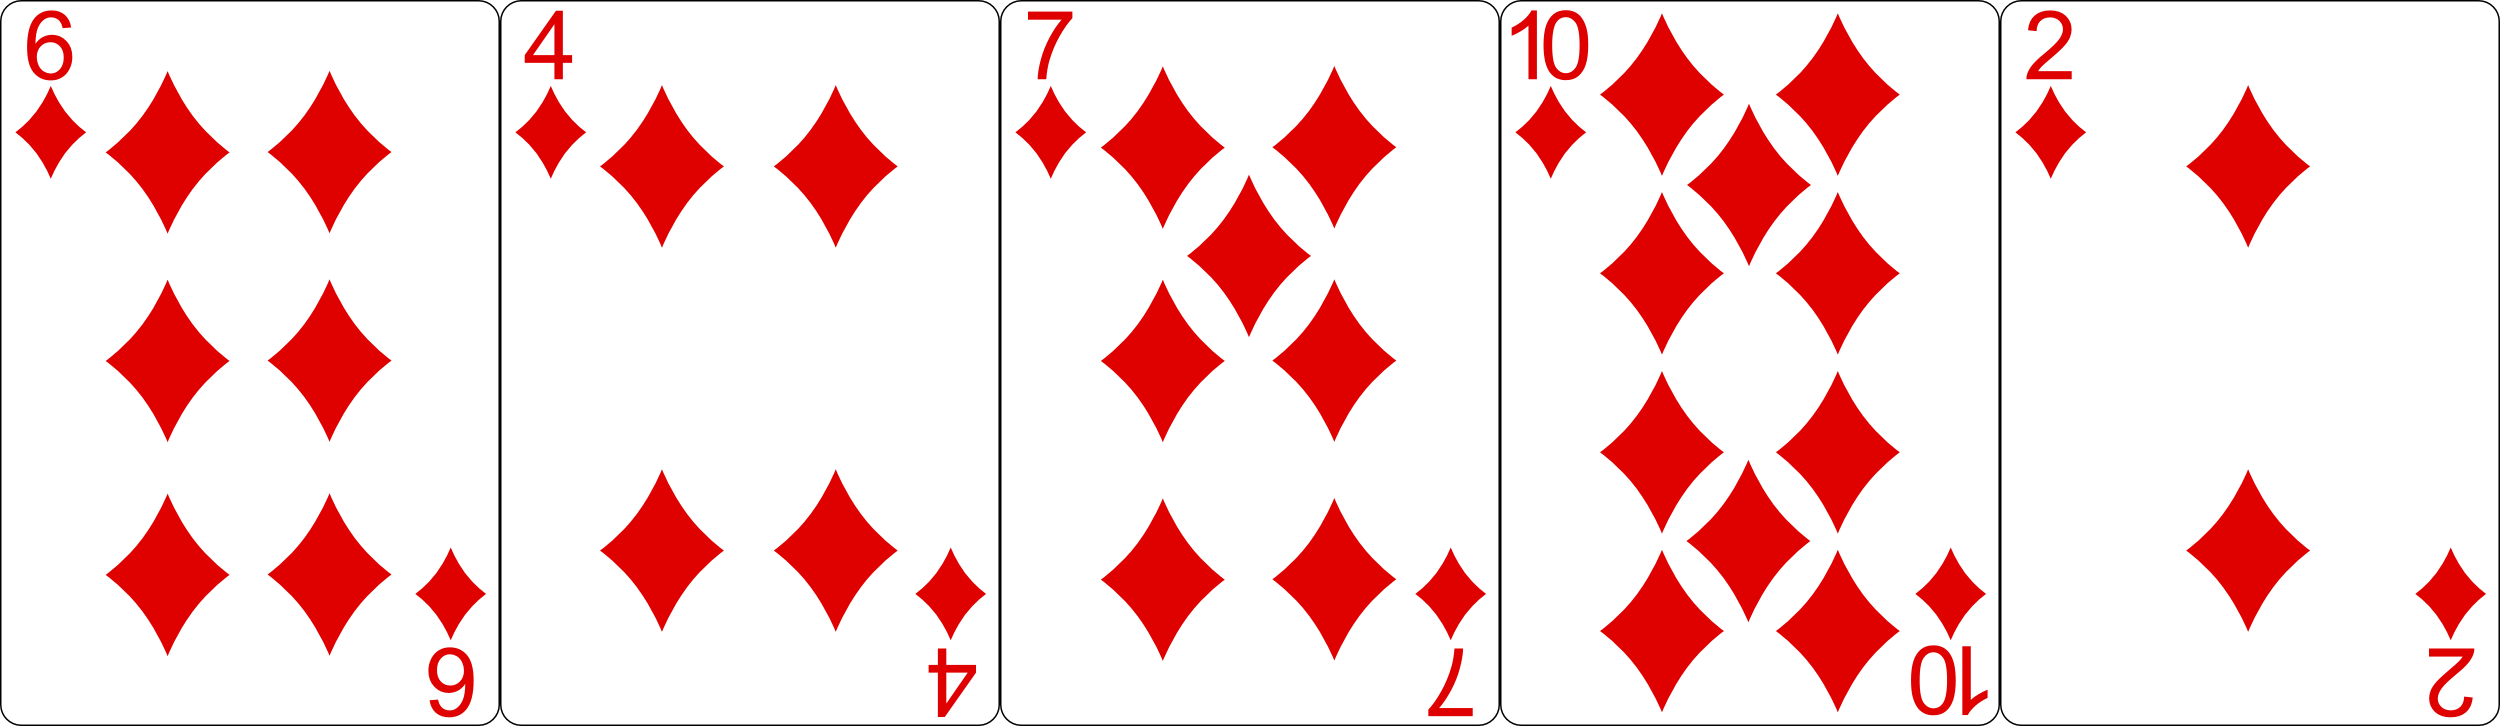
\includegraphics[width=\textwidth]{../img/w05-hands/flush.png}
 \end{minipage}
 \begin{minipage}[c]{\CardCaptionWidth}
  \caption{Färg: alla kort har samma färg.}
 \end{minipage}
\end{figure}

\begin{figure}[H]
 \begin{minipage}[c]{\CardWidth}
  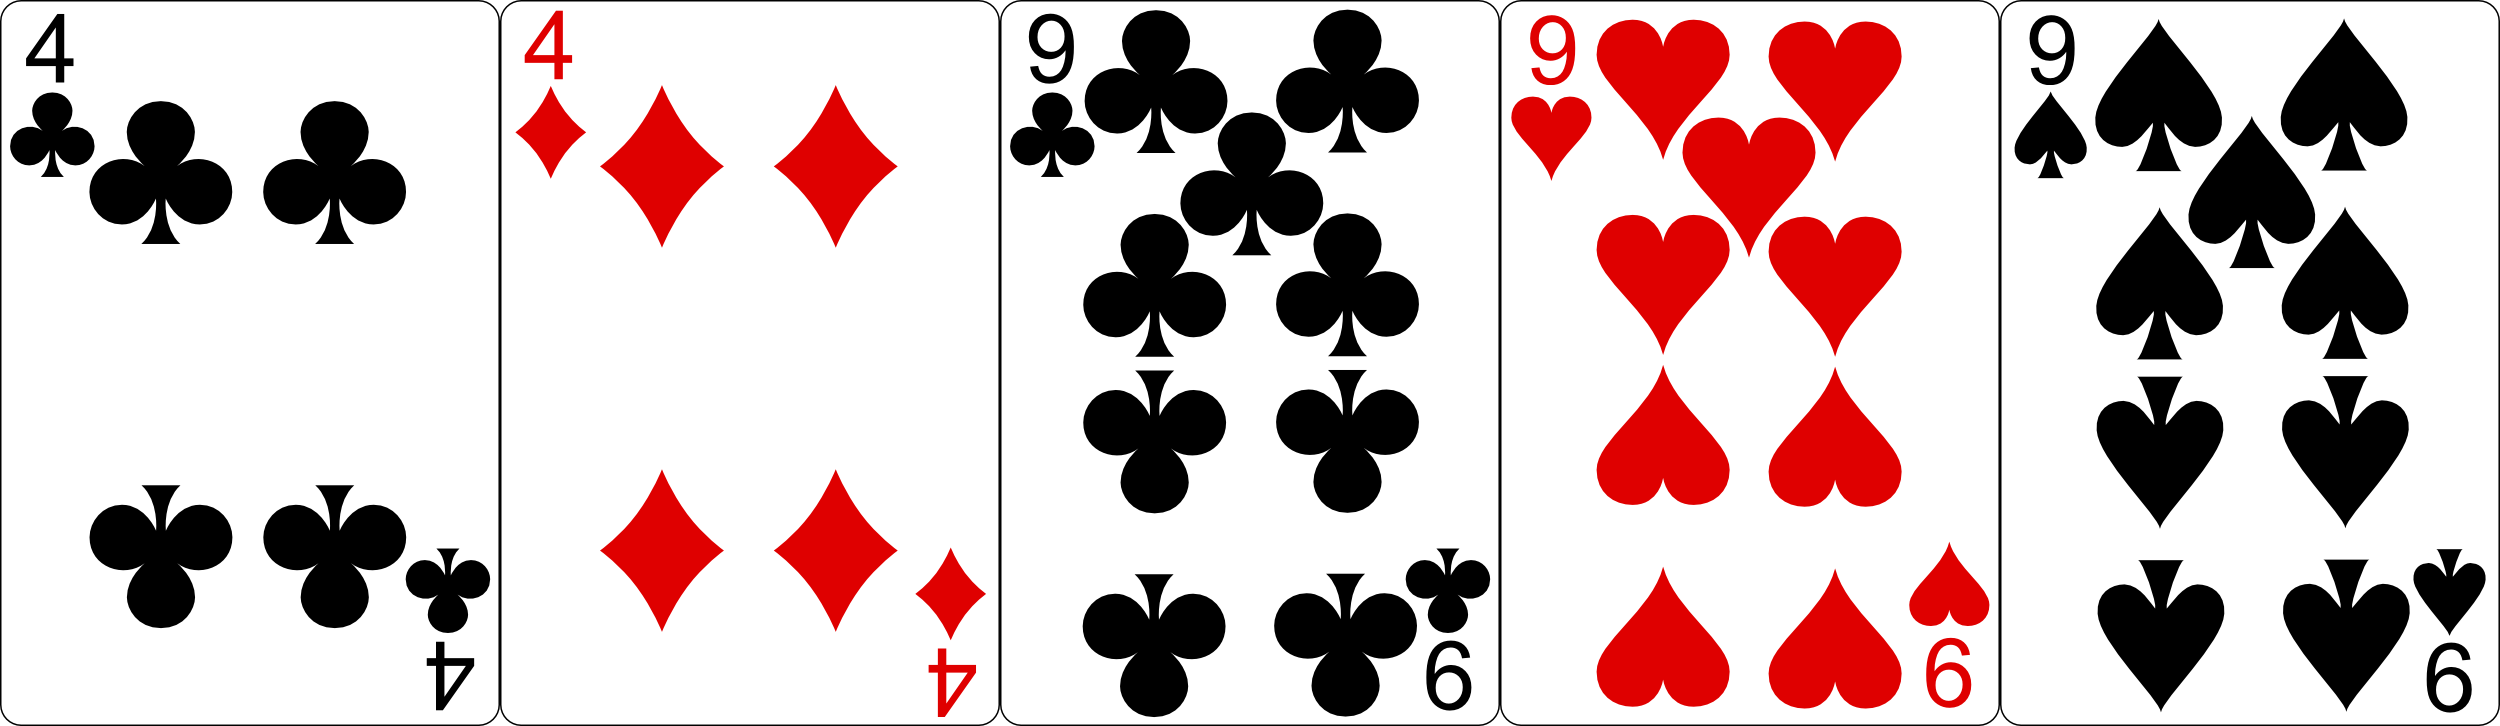
\includegraphics[width=\textwidth]{../img/w05-hands/fullhouse.png}
 \end{minipage}
 \begin{minipage}[c]{\CardCaptionWidth}
  \caption{Kåk: både triss och par.}
 \end{minipage}
\end{figure}

\begin{figure}[H]
 \begin{minipage}[c]{\CardWidth}
  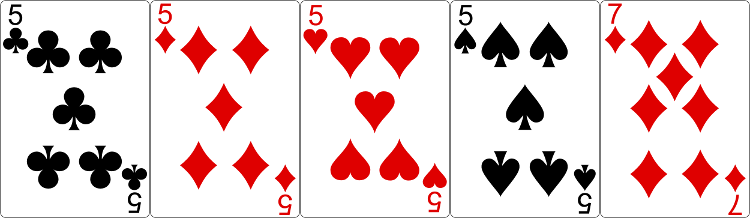
\includegraphics[width=\textwidth]{../img/w05-hands/fours.png}
 \end{minipage}
 \begin{minipage}[c]{\CardCaptionWidth}
  \caption{Fyrtal: fyra kort har samma valör.}
 \end{minipage}
\end{figure}

\begin{figure}[H]
 \begin{minipage}[c]{\CardWidth}
  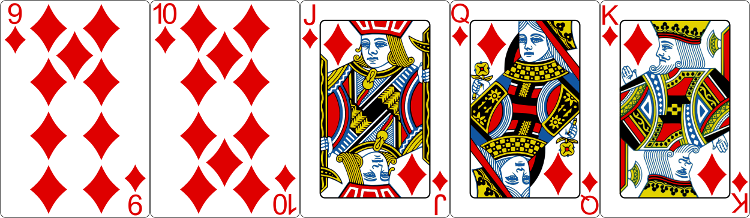
\includegraphics[width=\textwidth]{../img/w05-hands/straightflush.png}
 \end{minipage}
 \begin{minipage}[c]{\CardCaptionWidth}
  \caption{Färgstege: både stege och färg.}
 \end{minipage}
\end{figure}

\begin{figure}[H]
 \begin{minipage}[c]{\CardWidth}
  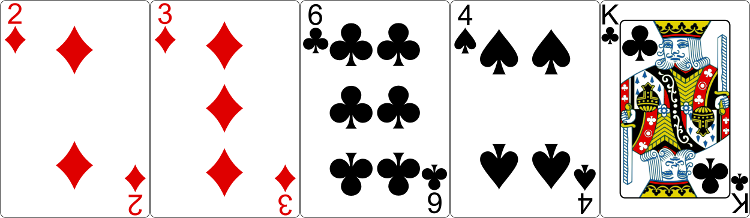
\includegraphics[width=\textwidth]{../img/w05-hands/none.png}
 \end{minipage}
 \begin{minipage}[c]{\CardCaptionWidth}
  \caption{Högt kort: inget mönster finns.}
 \label{lab:shuffle:last-picture}
  \end{minipage}
\end{figure}




\part{Andra läsperiodens laborationer och projekt}


%%!TEX encoding = UTF-8 Unicode
\chapter{Matriser, typparametrar}\label{chapter:W08}
Begrepp som ingår i denna veckas studier:
\begin{itemize}[noitemsep,label={$\square$},leftmargin=*]
\item matris
\item nästlad samling
\item nästlad for-sats
\item typparameter
\item generisk funktion
\item generisk klass
\item fri vs bunden typparameter
\item generiska datastrukturer
\item generiska samlingar i Scala\end{itemize}

%!TEX encoding = UTF-8 Unicode
%!TEX root = ../compendium2.tex

\Lab{\LabWeekEIGHT}

\begin{Goals}
\item Kunna skapa och använda matriser med hjälp av en generisk datatyp.
\item Kunna iterera över alla element i en matris.
\item Träna på algoritmkonstruktion.
\item Träna på hantering av både oföränderliga och förändringsbara objekt.
\item Använda en integrerad utvecklingsmiljö (IDE).
\end{Goals}

\begin{Preparations}
\item Gör övning {\tt \ExeWeekEIGHT} i kapitel \ref{chapter:W08}, speciellt uppgift \ref{exe:matrices:labprep}.

\item Läs igenom hela laborationen och studera den befintliga koden i \TODO \code{workspace}.

\item Läs appendix \ref{appendix:ide} och välj vilken IDE du ska använda (ScalaIDE/Eclipse eller IntelliJ IDEA). Säkerställ att du får igång en av dessa utvecklingsmijöer genom att köra hello-world-exemplet och sedan ladda ner och importera kursens \TODO workspace enligt instruktionerna i appendix \ref{appendix:ide}.
\end{Preparations}


\begin{figure}[H]
  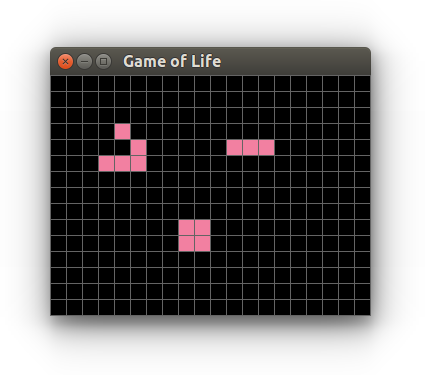
\includegraphics[width=0.8\textwidth]{../img/glider-blinker-block}

  \vspace{-2em}\caption{\label{lab:life:glider-blinker-block}Ett binärt, mörkt datauniversum av dimension $15  \times 20$. Cellkolonin innehåller tre cellgrupper: ett rymdskepp av typen \emph{glider}, en \emph{blinker} och ett \emph{block}.}
\end{figure}


\subsection{Bakgrund}

\emph{Game of Life} simulerar en koloni av encelliga organismer som lever, förökar sig och dör i en matris, enligt några enkla men väl valda regler som konstruerades av matematikern John Horton Conway på 1970-talet. Spelet går ut på att simulera flera generationer utifrån en startkonfiguration, även kallad \emph{cellkoloni}, där varje enskild cells överlevnad beror på dess omgivning. Spelet har inga medvetna spelare och om reglerna följs så kommer slutresultatet enbart bero på startkonfigurationen.

I \emph{Game of Life} består universum av en matris med celler som är antingen levande eller döda. Varje cell har 8 stycken \emph{grannar}, som utgörs av de närmsta omgivande cellerna vertikalt, horisontellt och diagonalt. Varje cells tillstånd i nästa generation bestäms av följande regler:
\begin{enumerate}[nolistsep]
    \item \textbf{Fortlevnad}. Om en levande cell har två eller tre grannar så lever den vidare.
    \item \textbf{Död}. Om en levande cell har mindre än två eller mer än tre grannar så dör den av underpopulation respektive överpopulation.
    \item \textbf{Födelse}. Om cellen är död och har exakt tre grannar så föds den och dess tillstånd ändras till levande, annars fortsätter den vara död.
\end{enumerate}

Flera cellkolonier uppvisar ett ''levande'' beteende där cellmatrisen koloniseras på intressanta vis när en sekvens av generationer visualiseras. Detta är ett exempel på \emph{emergent} beteende där komplexa, självorganiserade strukturer kan uppstå ur enkla förutsättningar.

Läs mer om \emph{Game of Life} på Wikipedia:
\begin{itemize}[noitemsep,topsep=0pt]
    	\item \url{https://en.wikipedia.org/wiki/Conway's_Game_of_Life}
    	\item \url{https://sv.wikipedia.org/wiki/Game_of_Life}
\end{itemize}


\subsection{Obligatoriska krav}

Följande funktionella krav ska uppfyllas av ditt program:
\begin{itemize}[nosep, label={$\square$},]
\item Levande celler ska ha den vackra rosa\footnote{\url{https://www.dsek.se/aktiva/grafiskprofil/farg.php}} RGB-färgen \code{(242, 128, 161)}.
\item Döda celler ska vara svarta som rymden.
\item Detta mörka universum med binära dataceller ska ritas i ett rutnät bestående av smala, stilfulla linjer, så som visas i fig. \ref{lab:life:glider-blinker-block}.
\item Tangenttryckningar och musklick ska fungera enligt följande hjälptext, som ska skrivas ut då programmet startas:
\begin{CodeSmall}
  val help = """
    Welcome to GAME OF LIFE!

    Click on cell to toggle.
    Press ENTER for next generation.
    Press SPACE to toggle play/stop.
    Press R to create random life.
    Press BACKSPACE to clear life.
    Close window to exit.
  """
\end{CodeSmall}
Då \emph{play} aktiveras med blankstegstangenten ska en kontinuerlig simulering av universum fortgå där varje ny generation visualiseras med en lagom fördröjning emellan generationer, tills simuleringen stoppas, t.ex. genom tryck ånyo på blankstegstangenten. Vid varje \emph{Enter}-tryck visas \emph{en} efterkommande generation och ev. pågående simulering stoppas. Vid musklick på en cell ska livstillståndet växlas från levande till död eller vice versa. Ett tryck på R ska ge slumpmässigt liv. Ett tryck på backstegstangenten ska rendera alla universums cellers död.

\end{itemize}

\vspace{1em}\noindent Din kod ska utformas enligt dessa design-krav:
\begin{itemize}[nosep, label={$\square$}]
\item Alla klasser och singelobjekt ska ligga i paketet \code{life}.
\item Det ska finnas en oföränderlig case-klass \code{Life} som representerar ett celluniversum med hjälp av en \code{Matrix[Boolean]} från uppgift \ref{exe:matrices:labprep} i veckans övning.
\item Det ska finnas en klass \code{LifeWindow} som visualiserar en  instans av klassen \code{Life} i ett  \code{introprog.PixelWindow} så som i fig. \ref{lab:life:glider-blinker-block}.
\end{itemize}


\subsection{Valbara krav -- välj minst ett}

Du ska implementera minst ett (gärna flera) av dessa krav:
\begin{itemize}[nosep, label={$\square$}]
\item Cellerna ska färgläggas i olika färger i enlighet med reglerna för nästa generation. Fortlevnad ska fortfarande vara vackert rosa och fortvarig död svart. Följande färger föreslås men välj andra om du tycker det blir finare:
\begin{CodeSmall}
  val UnderPopulated = java.awt.Color.cyan  // en giftig färg
  val OverPopulated  = java.awt.Color.red   // rödklämd av trängsel
  val WillBeBorn     = new java.awt.Color(40, 0, 0)  // snart levande
\end{CodeSmall}
Ge \code{LifeWindow} en klassparameter \code{isMultiColor} som styr om det blir mångfärgade celler eller om det bara finns rosa och svart som i grundkraven.

\item Om man trycker på \code{S} för \emph{Save} ska \code{introprog.Dialog.file("Save Life")} visas och, om användaren inte trycker \Button{Cancel}, det aktuella livet sparas med hjälp av \code{introprog.IO.saveString} i en textfil via metoden \code{toString} i \code{Life}.

\item Om man trycker på \code{O} för \emph{Open} ska \code{introprog.Dialog.file("Open Life")} anropas och ett nytt universum läsas in från textfil enligt lämpligt format. Inläsningen ska ske med hjälp av \code{introprog.IO.loadString} och tolkas till en \code{Life}-instans av en metod i kompanjonsobjektet med detta huvud:
\begin{CodeSmall}
def fromString(s: String, rowDelim: String="\n", alive: Char='0'): Life
\end{CodeSmall}
Testa med filen \texttt{glider-gun.txt} som ska ha följande innehåll på de första 11 raderna och totalt 32 rader där alla rader efter elfte raden innehåller tomt liv:
\begin{REPLnonum}
> head -11 glider-gun.txt
------------------------------------------
-------------------------0----------------
-----------------------0-0----------------
-------------00------00------------00-----
------------0---0----00------------00-----
-00--------0-----0---00-------------------
-00--------0---0-00----0-0----------------
-----------0-----0-------0----------------
------------0---0-------------------------
-------------00---------------------------
------------------------------------------
\end{REPLnonum}
\item Universum ska vara cirkulärt, d.v.s grannen vid kanten finns på andra sidan genom att indexeringen börjar om \Eng{wrapped} enligt modulo-räkning. Inför en klassparameter \code{isWrapped} i \code{Life} och en variabel \code{wrapped: Boolean} i kompanjonsobjektet \code{Life} som styr om fabriksmetoderna skapar ett universum som är cirkulärt eller ej, så att du lätt kan konfigurera detta. \emph{Tips:} Du har stor nytta av att använda \code|java.lang.Math.floorMod| i \code{apply}-metoden i \code{Life}; metoden \code{floorMod} räknar på lämpligt sätt med negativa värden, se dokumentationen för \code{Math}-paketet i JDK8.

\item Läs om varianter till \code{Game of Life} på Wikipedia och implementera alternativa regler som görs valbara genom konfigurering via \code{args}-parametern i \code{main}.

\item Skapa en klass \code{LifeStatistics} som genom väldigt många simuleringar ska ta reda på sannolikheten att en slumpmässig cellkoloni efter $n$ generationer fortfarande utvecklas, respektive är helt dött. Ingen visualisering med \code{PixelWindow} ska ske; endast antalet celler som lever vid generation $n$ och antalet celler som ändrades sedan generation $n - 1$ behöver registreras.

\end{itemize}




\subsection{Tips och förslag}

\begin{enumerate}[leftmargin=*]
\item Här är ett förslag på hur du kan utforma klassen \code{Life}:
\begin{CodeSmall}
package life

case class Life(val cells: Matrix[Boolean]) {

  /** Ger true om cellen på plats (row, col) är vid liv annars false.
    * Ger false om indexeringen är utanför universums gränser.
    */
  def apply(row: Int, col: Int): Boolean = ???

  /** Sätter status på cellen på plats (row, col) till value. */
  def updated(row: Int, col: Int, value: Boolean): Life = ???

  /** Växlar status på cellen på plats (row, col). */
  def toggled(row: Int, col: Int): Life = ???

  /** Räknar antalet levande grannar till cellen i (row, col).*/
  def nbrOfNeighbours(row: Int, col: Int): Int = ???

  /** Skapar en ny Life-instans med nästa generation av universum.
    * Detta sker genom att applicera funktionen \code{rule} på cellerna.
    */
  def evolved(rule: (Int, Int, Life) => Boolean = Life.defaultRule):Life = {
    var nextGeneration = Life.empty(cells.dim)
    cells.foreachIndex { (r,c) =>
      ???
    }
    nextGeneration
  }

  override def toString =
    cells.data.map(_.map(if (_) '0' else '-').mkString).mkString("\n")
}

object Life {
  /** Skapar ett universum med döda celler. */
  def empty(dim: (Int, Int)): Life = ???

  /** Skapar ett unviversum med slumpmässigt liv. */
  def random(dim: (Int, Int)): Life = ???

  /** Implementerar reglerna enligt Conways Game of Life. */
  def defaultRule(row: Int, col: Int, current: Life): Boolean = ???
}
\end{CodeSmall}
Du har nytta av metoden \code{copy} när du implementerar \code{updated} och \code{toggled}. Metoden \code{nbrOfNeighbours} har du nytta av när du ska implementera \code{defaultRule}. När du ska implementera \code{random} har du nytta av metoden \code{foreachIndex} i \code{Matrix[T]}.
Om du som i förslaget ovan låter \code{evolved} ta uppdateringsregeln som en funktionsparameter blir det lättare att konfigurera vilka regler som ska gälla och därmed blir det även lättare att skapa varianter av \emph{Game of Life} genom att införa nya regler i kompanjonsobjektet (se en av de valfria uppgifterna med vidare hänvisning till Wikipedia).

\item Här är ett förslag på hur du kan utforma klassen \code{LifeWindow}:
\begin{CodeSmall}
package life

import introprog.PixelWindow
import introprog.PixelWindow.Event

class LifeWindow(rows: Int, cols: Int){
  import LifeWindow._ // importera konstanter för cellstorlek, färger, etc.

  var life = Life.empty(rows, cols)
  val window: PixelWindow = ???
  var quit = false
  var play = false

  def drawGrid(): Unit = ???

  def drawCell(row: Int, col: Int): Unit = ???

  def update(newLife: Life): Unit = {
    val oldLife = life
    life = newLife
    life.cells.foreachIndex{ ??? }
  }

  def handleKey(key: String): Unit = ???

  def handleClick(pos: (Int, Int)): Unit = ???

  def loopUntilQuit(): Unit = while (!quit) {
    val t0 = System.currentTimeMillis
    if (play) update(life.evolved())
    window.awaitEvent(EventMaxWait)
    while (window.lastEventType != PixelWindow.Event.Undefined) {
      window.lastEventType match {
        case Event.KeyPressed  =>  handleKey(window.lastKey)
        case Event.MousePressed => handleClick(window.lastMousePos)
        case Event.WindowClosed => quit = true
        case _ =>
      }
      window.awaitEvent(EventMaxWait)
    }
    val elapsed = System.currentTimeMillis - t0
    Thread.sleep((NextGenerationDelay - elapsed) max 0)
  }

  def start(): Unit = { drawGrid(); loopUntilQuit() }
}
\end{CodeSmall}

\item \textbf{Dra nytta av den IDE du valt.} Det finns många användbara finesser i en integrerad utvecklingsmiljö. Orientera dig om grunderna genom att läsa appendix \ref{appendix:ide}. Lär dig några viktiga kortkommandon och studera hur du får igång debuggern. Prova att i debuggern sätta brytpunkter, stega dig fram och avläsa variablers värden.
\end{enumerate}

\noindent\TODO Är det för mycket tips? Eller behövs mer tips för att labben ska gå smidigt?


%\chapter{Matriser}
\begin{itemize}[nosep]
\item matriser
\item nästlade for-satser
\item designexempel: Tre-i-rad
\item matriser i Java vs Scala\end{itemize}
%!TEX encoding = UTF-8 Unicode

%!TEX root = ../compendium2.tex


\Lab{\LabWeekNINE}
\begin{Goals}
%!TEX encoding = UTF-8 Unicode
%!TEX root = ../compendium2.tex

%\item Kunna använda en integrerad utvecklingsmiljö (IDE).
%\item Kunna använda färdiga funktioner för att läsa till, och skriva från, textfil.
%\item Kunna använda enkla case-klasser.
%\item Kunna skapa och använda enkla klasser med föränderlig data.
\item Kunna skapa och använda nyckel-värde-tabeller med samlingstypen \code{Map}.
\item Kunna skapa och använda mängder med samlingstypen \code{Set}.
\item Förstå skillnaden mellan en ordnad sekvens och en mängd.
\item Förstå likheter och skillnader mellan en sekvens av par och en nyckel-värde-tabell. 
\item Kunna implementera algoritmer som använder nästlade strukturer. 
%\item Kunna skapa en ny samling från en befintlig samling.
%\item Förstå skillnaden mellan kompileringsfel och exekveringsfel.
%\item Kunna felsöka i små program med hjälp av utskrifter.
%\item Kunna felsöka i små program med hjälp av en debugger i en IDE.

\end{Goals}

\begin{Preparations}
\item \DoExercise{\ExeWeekSEVEN}{09}
%\item Läs om integrerade utvecklingsmiljöer i appendix \ref{appendix:ide}.
%\item Välj vilken IDE du vill använda på denna lab. %Om du inte vet vilken, välj \textbf{Eclipse} med ScalaIDE, som flest handledare känner väl till.
%\item Bekanta dig med utvecklingsmiljön genom att skapa ett nytt projekt och gör ett ''Hello World''-program.
%\item Ladda hem kursens \emph{workspace} enligt instruktioner i appendix \ref{subsubsection:download--import-workspace} och kontrollera så att du med \emph{Run} kan köra igång de båda ofärdiga \code{main}-metoderna i projektet \code{w04_pirates} inifrån din IDE. Om du inte får rätt på \emph{Run Configuration...} etc. så fråga någon om hjälp.
\item Läs igenom hela laborationen.
%\item {\"O}ppna Scala IDE i Eclipse enligt intruktionerna XX.
%\item Skapa ett projekt och skapa ett \code{object Hello} med en \code{main}-metod enligt XY.
%\item Skriv ut en h{\"a}lsning till terminalen med \code{println("...")} och testk{\"o}r programmet genom att markera filnamnet i projektmenyn och trycka p{\aa} den gr{\"o}na pilen. Kontrollera att h{\"a}lsningen skrivs ut!
\end{Preparations}


\subsection{Bakgrund}

Denna uppgift handlar om analys av naurligt språk \Eng{Natural Language Processing, NLP}. Språkanalys bygger ofta på statistik över förekomsten av olika ord i långa texter. Du ska skriva kod, som utifrån en lång text, till exempel en bok, kan hjälpa dig att svara på denna typ av frågor:
\begin{itemize}[noitemsep]
\item Hur vanligt är ett visst ord i en given text?
\item Vilket är det vanligaste ordet som följer efter ett visst ord?
\item Hur kan man generera ordsekvenser som liknar ordföljden i en given text?
\end{itemize}

\noindent För att kunna svara på sådana frågor ska du skapa frekvenstabeller och även så kallade \emph{n-gram}; sekvenser av $n$ ord som förekommer i följd i en text. Exempel på några 2-gram (kallas även \emph{bigram}) som finns i föregående mening: (för, att), (att, kunna), (kunna, svara), (svara, på), (på, sådana), och så vidare.\footnote{Du kan undersöka olika n-gram i en stor mängd böcker med hjälp av Googles n-gram-viewer: \url{https://books.google.com/ngrams/}}

\subsection{Obligatoriska uppgifter}

Du ska bygga ditt program med en editor, t.ex. VS \texttt{code}, och kompilera din kod i terminalen med \code{scalac} eller med hjälp av byggverktyget \code{sbt}. Medan du steg för steg utvecklar ditt program, ska du parallellt göra experiment i REPL för att undersöka hur du kan använda samlingsmetoder för att lösa uppgifterna.

Kod att utgå ifrån finns på github här: \url{https://github.com/lunduniversity/introprog/tree/master/workspace/w09_words}

Dessa ofärdiga kodfiler ligger i paketet \code{nlp}:
\begin{itemize}
  \item \href{https://github.com/lunduniversity/introprog/blob/master/workspace/w09_words/src/main/scala/nlp/FreqMapBuilder.scala}{\texttt{FreqMapBuilder.scala}} innehåller ett skelett till en klass för att, ord för ord, bygga en nyckel-värde-tabell som registrerar antalet förekomster av olika ord. Att implementera denna ingick i övningen du gjorde tidigare i veckan.

  \item \href{https://github.com/lunduniversity/introprog/blob/master/workspace/w09_words/src/main/scala/nlp/Text.scala}{\texttt{Text.scala}} innehåller ett skelett till en klass som kan göra textbehandling genom att analysera ord i en text.

  \item \href{}{\texttt{}} \href{https://github.com/lunduniversity/introprog/blob/master/workspace/w09_words/src/main/scala/nlp/Main.scala}{\texttt{Main.scala}} innehåller ett ofärdigt huvudprogramsexempel som du kan använda i laborationens senare del.
\end{itemize}

För att underlätta ditt arbetsflöde under det att du stegvis bygger upp din kod metod för metod, kan du med fördel använda byggverktyget \texttt{sbt} (se appendix \ref{appendix:build}) så här:

\begin{itemize}
  \item
    Med \code{sbt}-kommandot \code{console} startar du REPL innifrån \code{sbt} med dina klasser automatiskt  tillgängliga på classpath och du kan anropa de metoder som du gjort färdigt hittills medan du gör experiment inför nästa steg. När du ändrat något i din editor och vill experimentera med nya versionen så trycker du Ctrl+D och startar om REPL med \code{console} (pil-upp) och din kod kompileras om automatiskt.
  \item
    Med \code{sbt}-kommandot \code{~run} (notera tilde-tecknet) sker kompilering och körning av \code{main}-metoden automatiskt i terminalen varje gång du gör Ctrl+S i din editor.

\end{itemize}


\Task \emph{Skapa frekvenstabeller}. Du ska använda \code{FreqMapBuilder} från veckans övning för att skapa frekvenstabeller av typen \code{Map[String, Int]}, där nyckel-värde-paren i tabellen anger antalet förekomster av en viss sträng.

\Subtask Lägg klassen \code{FreqMapBuilder} i ett paket som heter \code{nlp} och kompilera.

\begin{figure}[H]
\scalainputlisting[numbers=left,basicstyle=\ttfamily\fontsize{10.5}{12.5}\selectfont]{../workspace/w09_words/src/main/scala/nlp/FreqMapBuilder.scala}
%\caption{Den ofärdiga klassen \code{FreqMapBuilder}.}
%\label{data:fig-freqmap}
\end{figure}

\Subtask Testa noga så att din \code{FreqMapBuilder} fungerar korrekt. Exempel på test i REPL:
\begin{REPL}
scala> import nlp._

scala> val fmb = FreqMapBuilder("hej", "på", "dej")
fmb: nlp.FreqMapBuilder = nlp.FreqMapBuilder@458f85ef

scala> fmb.add("hej")

scala> fmb.toMap
res0: Map[String,Int] = Map(på -> 1, hej -> 2, dej -> 1)

scala> (1 to Short.MaxValue).foreach(i => fmb.add(i.toString))

scala> fmb.toMap.size
res1: Int = 32770

scala> fmb.toMap
res2: Map[String,Int] = Map(10292 -> 1, 19125 -> 1, 26985 -> 1, 29301 -> 1, 5451 -> 1, 4018 -> 1, 31211 -> 1, 17319 -> 1, 20778 -> 1, 25285 -> 1, 17079 -> 1, 9936 -> 1, 13172 -
\end{REPL}

\noindent I kommande uppgifter ska du steg för steg skapa och testa case-klassen \code{Text}. %figur \ref{data:fig-text}.

\begin{figure}[H]
\scalainputlisting[numbers=left,basicstyle=\ttfamily\fontsize{10.4}{12.5}\selectfont]{../workspace/w09_words/src/main/scala/nlp/Text.scala}
%\caption{Den ofärdiga klassen \code{Text}.}
%\label{data:fig-text}
\end{figure}





\Task \emph{Dela upp en sträng i ord}. Du ska implementera medlemmen \code{words}. Den ska innehålla en vektor med alla ord i \code{source}, utan andra tecken än bokstäver.
Detta åstadkommer du genom att utgå ifrån strängen \code{source} och i tur och ordning göra följande:
\begin{enumerate}%[nolistsep, noitemsep]
\item byta ut alla tecken i \code{source} för vilka \code{isLetter} är falskt mot \code{' '}
\item dela upp strängen från föregående steg i en array av strängar med \code{split(' ')}
\item filtrera bort alla tomma strängar
\item gör om alla bokstäver i alla strängar till små bokstäver
\item gör om arrayen till en sekvens av typen \code{Vector[String]}.
\end{enumerate}

\noindent Testa så att \code{words}, och de värden som använder \code{words}, fungerar i REPL:
\begin{REPL}
scala> val t = Text("Gurka är ingen tomat, men gurka är en grönsak.")

scala> t.words
res1: Vector[String] =
  Vector(gurka, är, ingen, tomat, men, gurka, är, en, grönsak)

scala> t.distinct
res2: Vector[String] =
  Vector(gurka, är, ingen, tomat, men, en, grönsak)

scala> t.wordSet
res3: Set[String] = Set(grönsak, är, gurka, men, ingen, tomat, en)

scala> t.wordsOfLength(5)
res4: Set[String] = Set(gurka, ingen, tomat)

\end{REPL}



\Task Du ska nu skapa ordfrekvenstabellen \code{wordFreq} genom att registrera ordförekomster med hjälp av \code{FreqMapBuilder}. Tabellen \code{wordFreq} ska bestå av nyckelvärdepar \code{w -> f} där \code{f} är antalet gånger ordet \code{w} förekommer i \code{words}. Testa \code{wordFreq} genom att ladda ner boken ''Skattkammarön'' skriven av Robert Louis Stevenson\footnote{Copyright för denna bok har gått ut, så du gör dig inte skyldig till piratkopiering (i juridisk mening).} och undersök frekvensen för olika vanliga ord. Vilket ord är vanligast? Näst vanligast?

\begin{REPL}[basicstyle=\color{white}\ttfamily\fontsize{9}{11}\selectfont]
scala> val piratbok = Text.fromURL("https://fileadmin.cs.lth.se/pgk/skattkammaron.txt")
piratbok: nlp.Text = Text(Herr Trelawney, doktor Livesey och de övriga herrarna har bett mig att skriva ner alla omständigheter kring Skattkammarön, ...

scala> piratbok.words.size
res0: Int = 69438

scala> piratbok.wordFreq("pirat")
res1: Int = 7
\end{REPL}
Länkar till böcker i UTF-8-format som du kan använda i dina tester:
\begin{itemize}%[nolistsep,noitemsep]
\item ''Skattkammarön'' av R. L. Stevenson: \\\url{https://fileadmin.cs.lth.se/pgk/skattkammaron.txt}
\item ''Inferno'' av August Stringberg: \\\url{https://fileadmin.cs.lth.se/pgk/inferno.txt}
\item ''Pride and Prejudice'' av Jane Austen: \\\url{https://fileadmin.cs.lth.se/pgk/prideandprejudice.txt}
\item Projekt Gutenberg med många fritt tillgängliga böcker i textformat: \\\url{https://www.gutenberg.org/}
\end{itemize}






\Task Implementera metoden \code{ngrams} som ger en sekvens med alla ordföljder i $n$ steg. \emph{Tips:} På veckans övning ingick att undersöka hur metoden \code{sliding} fungerar, med vilken du kan skapa $n$-gram. Gör \code{toVector} på resultatet från \code{sliding}. Testa noga så att \code{ngrams} och \code{bigrams} fungerar korrekt innan du går vidare.
\begin{REPL}
scala> piratbok.ngrams(3).take(2)
res1: scala.collection.immutable.Vector[Vector[String]] =
Vector(Vector(herr, trelawney, doktor), Vector(trelawney, doktor, livesey))

scala> piratbok.bigrams.take(2)
res2: scala.collection.immutable.Vector[(String, String)] =
Vector((herr,trelawney), (trelawney,doktor))
\end{REPL}

\Task Implementera \code{followFreq}, som ska innehålla en nyckel-värde-tabell där värdet i sin tur är en frekvenstabell över de ord som kommer efter nyckeln.

Genom att analysera alla ordpar kan vi få fram vilket som är det vanligaste ordet som följer efter ett givet ord. Metoden \code{bigrams} ger oss alla ordpar \code{(w1, w2)} där \code{w2} följer efter \code{w1}. Vi kan spara statistiken över efterföljande ord i en nyckelvärdetabell med mappningarna \code{w -> f} där nyckeln \code{w} är ett ord  och värdet \code{f} är en frekvenstabell av typen \code{Map[String, Int]}. I frekvenstabellen lagrar vi frekvensen för alla de ord som följer efter \code{w}. Du ska alltså bygga en nästlad tabell av typen \code{Map[String, Map[String, Int]]}. Rita en bild av den nästlade strukturen.\Pen

Implementera metoden followFreq genom att utgå från nedan pseudokod:
\begin{Code}
val result = scala.collection.mutable.Map.empty[String, FreqMapBuilder]
for ((key, next) <- bigrams) {
  if (/* key finns redan definierad i result */)
    /* på "platsen" result(key): lägg till next i frekvenstabellen */
  else
    /* lägg till (key -> ny frekvenstabell med next) i result*/
}
result.mapValues(_.toMap).toMap // returnerar oföränderligt objekt
\end{Code}
Skriv uttryck för att ta reda på följande:\Pen

\Subtask Vilka ord brukar följa efter \emph{han} respektive \emph{hon} i Stevensons ''Skattkammarön''?

\Subtask Vilka ord brukar följa efter \emph{han} respektive \emph{hon} i Stringbergs ''Inferno''?

\Subtask Vilka ord brukar följa efter \emph{he} respektive \emph{she} i Austens ''Pride and Prejudice''?


\Task Skapa ett huvudprogram som rapporterar valfria, intressanta mått om orden i en text. Programmet ska ta textens källa som argument, givet som en URL eller ett filnamn. Skriv huvudprogrammet i filen \code{Main.scala} i ett singelobjekt med namnet \code{Main}. Exempel på en rapport som ditt huvudprogram kan generera finns nedan. Här ges även ett heltal som argument som styr topplistornas längd.
\begin{REPL}
> scala nlp.Main https://fileadmin.cs.lth.se/pgk/skattkammaron.txt 13

Källa: https://fileadmin.cs.lth.se/pgk/skattkammaron.txt

*** Antal ord: 69438

*** De 13 vanligaste orden och deras frekvens:
(och,3089), (jag,2007), (att,1594), (det,1382), (en,1262),
(i,1244), (som,1132), (på,1068), (han,1063), (var,990),
(med,854), (den,774), (av,740)

*** De 13 längsta orden och deras längd:
(besättningsmedlemmarnas,23), (befästningsanordningar,22),
(temperamentsuppvisning,22), (undsättningsexpedition,22),
(besättningsmedlemmarna,22), (försiktighetsåtgärder,21),
(undsättningsfartyget,20), (sjukdomsframkallande,20),
(husföreståndarinnans,20), (sjömansterminologin,19),
(parlamentärsflaggan,19), (bregravningsplatsen,19),
(tidvattenströmmarna,19)
\end{REPL}

\noindent Exempel på huvudprogram som kan skapa ovan utskrift:
\scalainputlisting[numbers=left,basicstyle=\ttfamily\fontsize{10.4}{12.5}\selectfont]{../workspace/w09_words/src/main/scala/nlp/Main.scala}

\subsection{Kontrollfrågor}

\begin{enumerate}
\item I vilken ordning hamnar elementen om man anropar \code{distinct} på en sekvens?

\item Om man itererar över en mängd, i vilken ordning behandlas elementen?

\item Ge exempel på när är det lämpligt att använda en mängd i stället för en sekvens av distinkta värden?

\item Är alla nycklar i en nyckel-värde-tabell garanterat unika?

\item Är alla värden i en nyckel-värde-tabell garanterat unika?

\item LTH-teknologen Oddput Clementin vill summera längden på varje sträng i en mängd och skriver:
\begin{REPL}
scala> Set("hej", "på", "dej").map(_.length).sum
res0: Int = 5
\end{REPL}
Varför blir det fel? Hur kan Oddput åtgärda problemet?
\end{enumerate}

\subsection{Frivilliga uppgifter}

\Task Bygg vidare på klassen \code{Text} och implementera nedan metod som ska ge ett slumpmässigt ord ur \code{wordSet}. Varje ord ska förekomma med lika stor sannolikhet.
\begin{Code}
def randomWord: String = ???
\end{Code}

\Task \label{task:words:randomSeq} Med NLP kan man generera slumpmässiga meningar som statistiskt sett liknar ''riktiga'', människoskapade meningar.

Implementera metoden \code{randomSeq(firstWord, n)} nedan i klassen \code{Text}. Den ska ge en sekvens $w_{1}, w_{2}, ..., w_{n}$  där $w_{1}$ är \code{firstWord} och $w_{i+1}$ är något slumpmässigt ord som är draget bland de ord som följer efter $w_{i}$. Detta kan du åstadkomma genom att varje efterföljande ord $w_{i+1}$ väljs ur \code{keys.toVector} för den \code{followFreq}-tabell som hör till $w_{i}$. Orden ska dras med rektangelfördelad sannolikhet ur efterföljandemängden.
\begin{Code}
def randomSeq(firstWord: String, n: Int): Vector[String] = ???
\end{Code}
%\emph{Tips:} Ett sätt att garanterat välja slumpmässigt element med rektangelfördelning ur en sekvens är att använda metoden \code{scala.util.Random.shuffle} som tar en sekvens som argument och genererar en ny sekvens av samma typ, men med elementen ordnade i slumpmässig ordning på ett välblandat sätt, där varje möjlig ordning är lika sannolik.

\Task \label{task:words:mostCommonSeq} För att dina datorgenererade meningar verkligen ska likna mänskilgt språk kan vi skapa de mest sannolika meningarna av olika längder ur vår analys av ordfrekvenser.

Lägg till metoden \code{mostCommonSeq} i klassen \code{Text} enligt nedan:
\begin{Code}
def mostCommonSeq(firstWord: String, n: Int): Vector[String] = ???
\end{Code}
\Subtask Implementera metoden så att resultatet blir en sekvens med \code{n} ord. Sekvensen ska börja med \code{firstWord} och därefter följas av det ord som är det \emph{vanligaste} efterföljande ordet efter \code{firstWord}, och därpå det vanligaste efterföljande ordet efter det, etc. \emph{Tips:} Använd en lokal variabel \code{val result} som är en ArrayBuffer till vilken du i en \code{while}-loop lägger de efterföljande orden.

\Subtask Jämför de slumpmässiga sekvenserna med sekvenser genererade med \code{randomSeq} i uppgift \ref{task:words:randomSeq}. Vilka sekvenser liknar mest ''riktiga'' meningar?


\Task Använd befintliga samlingsmetoder i stället för \code{FreqMapBuilder} för att registrera efterföljande ord.

\Subtask Undersök i REPL hur metoden \code{groupBy(x => x)} fungerar då den appliceras på en samling med strängar. Sök efter och studera dokumentationen för \code{groupBy}.

\Subtask Undersök i REPL hur metoden \code{mapValues} fungerar då den appliceras på en nyckel-värde-tabell där värdet är en samling. Sök efter och studera dokumentationen för \code{mapValues}.

\Subtask Inför värdet \code{lazy val wordFreq2}. Den ska ge samma resultat som \code{wordFreq} men men implementeras med hjälp av \code{groupBy} och \code{mapValues} i stället för \code{FreqMapBuilder}.

\Subtask\Uberkurs Jämför prestanda mellan \code{wordFreq2} och \code{wordFreq}. Vilken är snabbast för stora texter? Är skillnaden stor?

\Subtask Inför värdet \code{lazy val followsFreq2}. Den ska ge samma resultat som \code{followsFreq} men implementeras med hjälp av \code{groupBy} och \code{mapValues} i stället för \code{FreqMapBuilder}.
Denna uppgift är ganska knepig. Experimentera dig fram i REPL, och bygg upp en lösning steg för steg. \emph{Tips:}
\begin{Code}
bigrams
  .groupBy(???)
  .mapValues(_.map(???).groupBy(???).mapValues(???))
\end{Code}

\Subtask\Uberkurs Jämför prestanda mellan \code{followsFreq2} och \code{followsFreq}. Vilken är snabbast för stora texter? Är skillnaden stor?


\Task\Uberkurs \emph{Gör \code{FreqMapBuilder} generisk.} Senare i kursen ska vi se hur man kan skapa s.k. generiska datastrukturer med hjälp av typparametrar. Denna uppgift går händelserna i förväg och tjuvkikar på hur en generisk klass kan se ut.

\Subtask Studera \code{FreqMapBuilder} och identifiera allt i den klassen som är specifikt för typen \code{String}.

\Subtask Inför en typparameter \code{A} inom hakparenteser efter klassnamnet och använd sedan \code{A} i stället för \code{String} i alla metoder.

\Subtask Testa så att din generiska frekvenstabellbyggare fungerar på sekvenser som innehåller annat än strängar.


%\chapter{Sökning, Sortering}\label{chapter:W10}
\begin{itemize}[nosep]
\item algoritm: LINEAR-SEARCH
\item algortim: BINARY-SEARCH
\item algoritmisk komplexitet
\item sortering till ny vektor
\item sortering på plats
\item algoritm: INSERTION-SORT
\item algoritm: SELECTION-SORT
\end{itemize}
%!TEX encoding = UTF-8 Unicode
%!TEX root = ../compendium2.tex

\Teamlab{\LabWeekTEN}

\begin{Goals}
%!TEX encoding = UTF-8 Unicode
%!TEX root = ../compendium2.tex

\item Kunna använda arv.
\item Kunna göra överskuggning av medlemmar i en supertyp.
%\item Kunna referera till medlemmar i superklassen med \code{super} vid överskuggning.
\item Kunna förklara begreppet dynamisk bindning.
\item Kunna använda abstrakta klasser och skapa en klasshierarki.

\end{Goals}

\begin{Preparations}
\item Gör övning {\tt \ExeWeekNINE} i kapitel \ref{exe:W09}, speciellt uppgift \ref{exe:inheritance:labprep-pair}.
\item Läs dokumentationen för \code{introprog.BlockGame}.
\item Läs igenom hela laborationen och förbered dig inför första gruppmötet.
%!TEX encoding = UTF-8 Unicode
%!TEX root = compendium.tex
\item 
Diskutera i din samarbetsgrupp hur ni ska dela upp koden mellan er i flera olika delar, som ni kan arbeta med var för sig. En sådan del kan vara en klass, en trait, ett objekt, ett paket, eller en funktion. 
\item
Varje del ska ha en \emph{huvudansvarig} individ. 
\item
Arbetsfördelningen ska vara någorlunda jämnt fördelad mellan gruppmedlemmarna.
\item
När ni redovisar er lösning ska ni börja med att redogöra för handledaren hur ni delat upp koden och vem som är huvudansvarig för vad. 
\item
Den som är huvudansvarig för en viss del redovisar den delen.
\item 
Grupplaborationer görs i huvudsak som hemuppgift. Salstiden används primärt för redovisning.
\item Träffas i din samarbetsgrupp och diskutera ert arbetssätt utifrån följande frågeställningar:
\begin{itemize}[nolistsep]
  \item Vilka krav ska ni implementera?
  \item Hur ska ni jobba med gemensamma koddelar?
  \item Hur ska ni dela med er av de koddelar som ni utvecklar var för sig?
\end{itemize}

\end{Preparations}

\subsection{Bakgrund}

Spelet \emph{Snake}\footnote{Även kallat ''masken''. \url{https://sv.wikipedia.org/wiki/Snake}} blev mäkta populärt i Sverige redan på 1980-talet, ofta spelat på den legendariska datorn ABC80. Spelet finns i flera varianter, både för en spelare och som duell mellan två spelare. Varje spelare styr en mask med huvud och svans som hela tiden rör sig framåt. Det gäller att undvika att köra in i en masksvans och att samla poäng t.ex. genom att äta äpple.

Figur~\ref{fig:snake-game} visar en startdialog där man kan välja antal spelare, samt ett exempel på spel med en och två spelare. I varianten för en spelare närmar sig maskens huvud äpplet och lyckas kanske äta det om spelaren styr rätt.  I varianten för två spelare vinner grön mask eftersom den blåa masken råkade köra in i den gröna maskens svans.
\begin{figure}[H]
\begin{minipage}{0.45\textwidth}
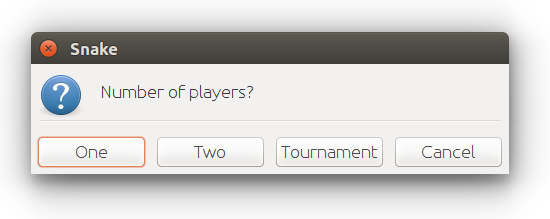
\includegraphics[width=1.0\textwidth]{../img/snake-start}

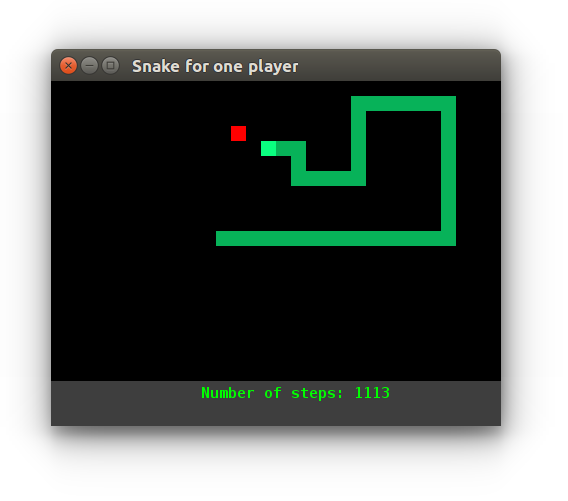
\includegraphics[width=1.0\textwidth]{../img/snake-oneplayer}
\end{minipage}
\begin{minipage}{0.5\textwidth}
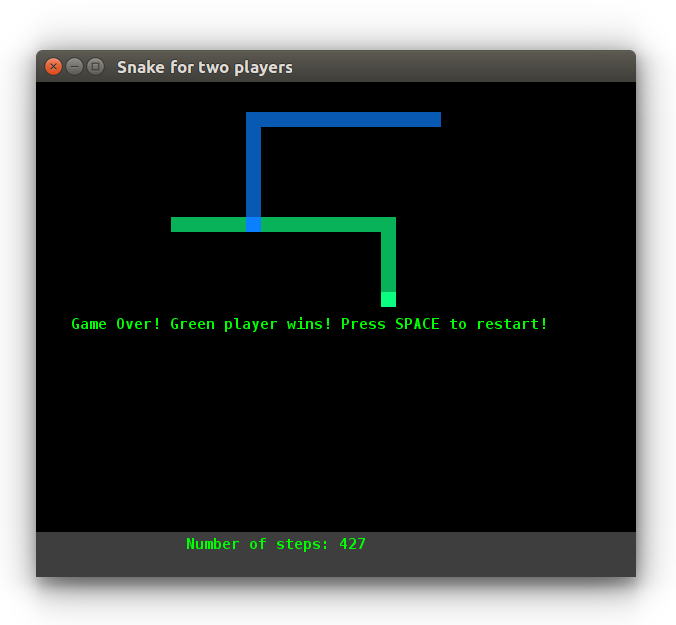
\includegraphics[width=1.0\textwidth]{../img/snake-twoplayer}
\end{minipage}
\caption{Spelet snake för en spelare med äpple och för två spelare utan äpple. \label{fig:snake-game}}
\end{figure}

\subsection{Obligatoriska funktionella krav}

Följande funktionella krav ska uppfyllas av ert program om ni är sex personer i gruppen. Om ni är färre ingår de obligatoriska krav som visas i tabell \ref{lab:snak:table-reqt}.
%\footnote{Om någon student, p.g.a. långvarig sjukdom eller annat giltigt skäl, genomför laborationen själv i efterhand som en individuell laboration ska följande krav implementeras på egen hand: \code{Player}, \code{OnePlayerGame}, \code{Snake}, \code{Apple}.}
\begin{itemize}[nosep, label={$\square$},]
\item \textbf{\texttt{Player}}. Det ska finnas spelare som motsvarar mänskliga användare och som har ett namn och fyra tangenter som den kan spela med. Varje spelare har en egen orm som den kan styra med sina tangenter.

\item \textbf{\texttt{Snake}}. Det ska finnas ormar. En orm består av ett antal block, där det främsta blocket kallas huvud och resten av blocken kallas svans. Huvudet har en ljusare färg än kroppen. Svansens längd ökar under spelets gång. En orm rör sig i en viss riktning och varje spelare kan ändra riktningen på sin orm med sina tangenter, i en av fyra riktningar \code{North}, \code{South}, \code{East} eller \code{West}.

\item \textbf{\texttt{Apple}}. Det ska finnas (minst ett) äpple. Ett äpple består av ett rött block och finns på en slumpvis position. Ett äpple kan ätas av en orm om ormens huvud träffar äpplet. Varje gång ett äpple äts upp av en orm så teleporteras äpplet till en ny position och kan ätas igen.

\item \textbf{\texttt{Banana}}. Det ska finnas (minst en) banan. En banan består av tre vertikala gula block och finns på en slumpvis position. En banan äts upp av en orm om ormens huvud träffar bananen. Varje gång en banan äts upp av en orm så teleporteras bananen till en ny slumpvis position och kan ätas igen.

\item \textbf{\texttt{Monster}}. Det ska finnas (minst ett) monster. Ett monster består av fem rosa block i kryssform.  Ett monster föds på en slumpvis position och rör sig i en riktning som bestäms vid monstrets födelse. Ett orm blir uppäten och dör om ormens huvud nuddar ett monsterblock .

\item \textbf{\texttt{OneplayerGame}}. Det ska gå att spela ensam. I varianten med en spelare finns en orm och minst ett äpple (och ev. även bananer och monster). Varje gång användarens orm lyckas äta en frukt får användaren poäng. När ormen ätit ett visst antal äpplen, eller om ormen blivit uppäten av ett monster, är spelet slut och poängen visas. En ormsvans ska bli längre vid jämna tidsintervall eller om den äter frukt.

\item \textbf{\texttt{TwoplayerGame}}. Det ska gå att spela två och två. I varianten med två spelare finns två ormar. Det finns också äpplen, bananer och monster. Om en orm äter en banan blir dess svans längre. När ormen ätit ett visst antal äpplen, eller om ormen blivit uppäten av ett monster, är spelet slut och poängen visas. En ormsvans ska bli längre vid jämna tidsintervall eller om den äter frukt.

\item \textbf{\texttt{Settings}}. Inställningar för spelet ska vara konfigurerbara genom en textfil som laddas i början av spelet. Inställningar ska vara en kontextparameter.  

\end{itemize}
\begin{table}[H]
  \centering
  \caption{Krav som minst ska implementeras vid respektive gruppstorlek. Om du har särskilda skäl kan du efter godkännande från kursansvarig göra labben enskilt.  \label{lab:snak:table-reqt}}

\begin{tabular}{r | c c c c c c}
  Krav / Antal personer & 1       & 2       & 3       & 4       & 5       & 6 \\ \hline
  \texttt{Player}       & $\surd$ & $\surd$ & $\surd$ & $\surd$ & $\surd$ & $\surd$ \\
  \texttt{OnePlayerGame}& $\surd$ &         &         &         & $\surd$ & $\surd$ \\
  \texttt{TwoPlayerGame}&         & $\surd$ & $\surd$ & $\surd$ & $\surd$ & $\surd$ \\
  \texttt{Snake}        & $\surd$ & $\surd$ & $\surd$ & $\surd$ & $\surd$ & $\surd$ \\
  \texttt{Apple}        & $\surd$ &         & $\surd$ & $\surd$ & $\surd$ & $\surd$ \\
  \texttt{Banana}       &         &         &         & $\surd$ &         & $\surd$ \\
  \texttt{Monster}      &         &         & $\surd$ &         &         & $\surd$ \\
  \texttt{Settings}     & $\surd$ & $\surd$ & $\surd$ & $\surd$ & $\surd$ & $\surd$ \\
\end{tabular}
\end{table}

\subsection{Obligatoriska design-krav}

\begin{enumerate}[label={$\square$}, leftmargin=*]

\item Snake-spel ska gå att starta med huvudprogrammet nedan. Huvudprogrammet får ändras vid behov i enlighet med minimikrav vad gäller gruppstorlek i tabell \ref{lab:snak:table-reqt}, samt valbara extrakrav i avsnitt \ref{lab:snake:extra-reqts}, och era egna ideer.
\scalainputlisting{../workspace/w10_snake/src/main/scala/snake/Main.scala}

\item Spelet ska bygga vidare på \code{introprog.BlockGame} enligt typhierarkin i fig.~\ref{snake:fig:game-hierarchy}.

\begin{figure}[H]
\begin{center}
\newcommand{\TextBox}[1]{\raisebox{0pt}[1em][0.5em]{#1}}
\tikzstyle{umlclass}=[rectangle, draw=black,  thick, anchor=north, text width=3cm, rectangle split, rectangle split parts = 3]
\begin{tikzpicture}[inner sep=0.5em,scale=1.0, every node/.style={transform shape}]

  \node [umlclass, rectangle split parts = 1, xshift=0cm, yshift=4.5cm] (BaseType)  {
              \textit{\textbf{\centerline{\TextBox{\code{BlockGame}}}}}
%              \nodepart[align=left]{second}\code{def x: T} \newline \code{def y: T}
          };


  \node [umlclass, rectangle split parts = 1, xshift=0cm, yshift=3.0cm] (SubType)  {
              \textit{\textbf{\centerline{\TextBox{\code{SnakeGame}}}}}
%              \nodepart[align=left]{second}\code{val x: Int} \newline \code{val y: Int}
          };

\node [umlclass, rectangle split parts = 1, xshift=-3cm, yshift=1.0cm] (SubSubType1)  {
            {\textbf{\centerline{\TextBox{\code{OnePlayerGame}}}}}
%            \nodepart[]{second}\TextBox{\code{val dim: Int}}
        };

\node [umlclass, rectangle split parts = 1, xshift=3cm, yshift=1.0cm] (SubSubType2)  {
            {\textbf{\centerline{\TextBox{\code{TwoPlayerGame}}}}}
%            \nodepart[]{second}\TextBox{\code{val dim: Int}}
        };

\draw[umlarrow] (SubType.north) -- ++(0,0.5) -| (BaseType.south);
\draw[umlarrow] (SubSubType1.north) -- ++(0,0.5) -| (SubType.south);
\draw[umlarrow] (SubSubType2.north) -- ++(0,0.5) -| (SubType.south);

\end{tikzpicture}
\end{center}
\caption{Arvshierarki med klassen \code{introprog.BlockGame} som bastyp.}
\label{snake:fig:game-hierarchy}
\end{figure}


\item Ormar, monster och frukt ska utgå från bastypen \code{Entity} enligt typhierarkin i ~\ref{snake:fig:entity-hierarchy}.

\begin{figure}[H]
\begin{center}
\newcommand{\TextBox}[1]{\raisebox{0pt}[1em][0.5em]{#1}}
\tikzstyle{umlclass}=[rectangle, draw=black,  thick, anchor=north, text width=2.5cm, rectangle split, rectangle split parts = 3]
\begin{tikzpicture}[inner sep=0.5em,scale=1.0, every node/.style={transform shape}]

  \node [umlclass, rectangle split parts = 1, xshift=0.0cm, yshift=4.5cm] (BaseType)  {
              \textit{\textbf{\centerline{\TextBox{\code{Entity}}}}}
%              \nodepart[align=left]{second}\code{def x: T} \newline \code{def y: T}
          };


  \node [umlclass, rectangle split parts = 1, xshift=-3.0cm, yshift=2.5cm] (SubType1)  {
              \textit{\textbf{\centerline{\TextBox{\code{CanMove}}}}}
%              \nodepart[align=left]{second}\code{val x: Int} \newline \code{val y: Int}
          };

\node [umlclass, rectangle split parts = 1, xshift=-4.75cm, yshift=0.5cm] (SubSubType01)  {
            {\textbf{\centerline{\TextBox{\code{Snake}}}}}
%            \nodepart[]{second}\TextBox{\code{val dim: Int}}
};

\node [umlclass, rectangle split parts = 1, xshift=-1.5cm, yshift=0.5cm] (SubSubType02)  {
            {\textbf{\centerline{\TextBox{\code{Monster}}}}}
%            \nodepart[]{second}\TextBox{\code{val dim: Int}}
};


\node [umlclass, rectangle split parts = 1, xshift=3.0cm, yshift=2.5cm] (SubType2)  {
            \textit{\textbf{\centerline{\TextBox{\code{CanTeleport}}}}}
%            \nodepart[]{second}\TextBox{\code{val dim: Int}}
        };

\node [umlclass, rectangle split parts = 1, xshift=1.75cm, yshift=0.5cm] (SubSubType1)  {
            {\textbf{\centerline{\TextBox{\code{Apple}}}}}
%            \nodepart[]{second}\TextBox{\code{val dim: Int}}
        };

\node [umlclass, rectangle split parts = 1, xshift=5.0cm, yshift=0.5cm] (SubSubType2)  {
            {\textbf{\centerline{\TextBox{\code{Banana}}}}}
%            \nodepart[]{second}\TextBox{\code{val dim: Int}}
        };


\draw[umlarrow] (SubType1.north) -- ++(0,0.5) -| (BaseType.south);
\draw[umlarrow] (SubType2.north) -- ++(0,0.5) -| (BaseType.south);
\draw[umlarrow] (SubSubType1.north) -- ++(0,0.5) -| (SubType2.south);
\draw[umlarrow] (SubSubType2.north) -- ++(0,0.5) -| (SubType2.south);
\draw[umlarrow] (SubSubType01.north) -- ++(0,0.5) -| (SubType1.south);
\draw[umlarrow] (SubSubType02.north) -- ++(0,0.5) -| (SubType1.south);

\end{tikzpicture}
\end{center}
\caption{Arvshierarki med klassen \code{Entity} som bastyp.}
\label{snake:fig:entity-hierarchy}
\end{figure}


\item \code{Entity} representerar en varelse i ett spel och ska se ut så här:
\scalainputlisting{../workspace/w10_snake/src/main/scala/snake/Entity.scala}
% \begin{Code}
% trait Entity {
%   def draw():   Unit
%   def erase():  Unit
%   def update(): Unit
%   def reset():  Unit
% }
% \end{Code}
Metoderna \code{draw} resp. \code{erase} anropas vid ritning resp. radering. Metoden \code{reset} återställer ursprungstillståndet. Metoden \code{update} anropas en gång i varje runda i spel-loopen. Predikatet \code{isOccupyingBlockAt} ger sant om positionen \code{p} finns bland de block som varelsen ockuperar på skärmen.

\item \code{CanMove} representerar en entitet som kan röra sig i en viss hastighet, enligt:
\scalainputlisting{../workspace/w10_snake/src/main/scala/snake/CanMove.scala}

% \begin{Code}
% trait MovingEntity extends Entity {
%   def move(): Unit
%
%   var movesPerSecond: Double = 20.0
%
%   final def millisBetweenMoves(): Int =
%     (1000 / movesPerSecond).round.toInt max 1
%
%   private var _timestampLastMove: Long = System.currentTimeMillis
%   final def timestampLastMove = _timestampLastMove
%
%   override final def update(): Unit =
%     if (System.currentTimeMillis > _
%           timestampLastMove + millisBetweenMoves) {
%       _timestampLastMove = System.currentTimeMillis
%       move()
%     }
% }
% \end{Code}

\item \code{CanTeleport} representerar en entitet som finns på en viss plats men som efter ett visst antal uppdateringar utan förvarning teleporterar sig till en ny position:
\scalainputlisting{../workspace/w10_snake/src/main/scala/snake/CanTeleport.scala}

\item Det ska finnas en enumeration \code{State} i singelobjektet \code{SnakeGame} som representerar spelets övergripande tillstånd enligt följande:
\begin{Code}
package snake 

object SnakeGame:
  enum State:
    case Starting, Playing, GameOver, Quitting
  export State.* // gör alla tillstånd synliga i SnakeGame
\end{Code}

\item Vid varje runda i spelloopen ska följande logik exekveras. Denna kod placeras förslagsvis i \code{gameLoopAction}, se vidare \code{SnakeGame} i avsnitt \ref{lab:snake:tips}.
\begin{Code}
    if state == Playing && !isPaused then
      _iterationsSinceStart += 1
      entities.foreach(_.erase())
      entities.foreach(_.update())
      entities.foreach(_.draw())
      onIteration()
      if isGameOver then enterGameOverState()
\end{Code}

\item Det ska finnas ett singelobjekt \code{Colors} där alla färger som används i spelet samlas.

\item Filen \code{pairs.scala} ska enligt laborationsförberedelser i övningsuppgift   \ref{exe:inheritance:labprep-pair} på sidan \pageref{exe:inheritance:labprep-pair} innehålla
\code{Pair[T]}, \code{Dim}, \code{Pos}, \code{Dir}, \code{North}, \code{South}, \code{East}, \code{West}. Se workspace här:\\
\url{https://github.com/lunduniversity/introprog/tree/master/workspace/}

\item Klassen \code{Player} ska se ut som följer:

\end{enumerate}

\scalainputlisting[basicstyle=\ttfamily\fontsize{10.5}{13}\selectfont]
{../workspace/w10_snake/src/main/scala/snake/Player.scala}




\subsection{Valbara krav -- varje person ska välja minst ett}\label{lab:snake:extra-reqts}

Varje person i gruppen ska implementera \emph{minst ett} (gärna flera) av kraven nedan. Vid implementation av flera av dessa krav blir spelet väsentligt roligare.
\begin{itemize}[nosep, label={$\square$}]

\item \textbf{\code{Points}}. Inför ett poängsystem, där poängen beror på t.ex. längden på svansen, antalet steg, antalet svängar, antal uppätna äpplen, etc.

\item \textbf{\code{Highscore}}. Spelet ska visa en lista med de spelare som fått flest poäng.

\item \texttt{\textbf{Äpple}}. Om inte redan ingår bland obl. krav enl.~ \ref{lab:snak:table-reqt}.

\item \textbf{\code{Monster}}. Om inte redan ingår bland obl. krav enl. 
\ref{lab:snak:table-reqt}.

\item \textbf{\code{Banan}}. Om inte redan ingår bland obl. krav enl. 
\ref{lab:snak:table-reqt}.

\item \textbf{\code{SelfTailCrash}}. Om en spelare kör in i sin egen orms svans så är spelet förlorat. (Om detta krav ej implementeras så \emph{får} man köra igenom sin egen svans utan att något händer.)

\item \textbf{\code{BoundaryCrash}}. Om en spelare kör utanför spelplanen så är spelet förlorat. (Om detta krav ej implementeras så ska ormen fortsätta på andra sidan spelplanen när man når kanten.)

\item \textbf{\code{EnterPlayerName}}. Spelare kan ange sitt namn, t.ex. via en dialog eller genom argument till \code{main}. Namnet används i meddelandefältet vid poängräkning och i meddelanden om vem som vunnit.

\item \textbf{\code{TwoPlayerComp extends Competition}}. Två spelare ska kunna tävla i en bäst-av-$n$-matcher-tävling i en sekvens av \code{TwoPlayerGame.play}, där den som vinner flest matcher blir blir totalvinnare.

\item \textbf{\code{SinglePlayerComp extends Competition}}. Flera spelare ska kunna tävla i en-persons-Snake, där den som får flest poäng av $n$ \code{OnePlayerGame}-spel blir totalvinnare.

\item \textbf{\code{Tournament extends Competition}}. Många spelare ska kunna spela en turnering.\footnote{\url{https://en.wikipedia.org/wiki/Tournament}} Namnen på spelarna läses in från en textfil. Valbara varianter:

\begin{itemize}[nosep, label={$\square$}]
\item \textbf{\code{KnockOut extends Tournament}}. Det ska gå att spela en utslagsturnering, som avslutas med final efter semi-final, etc., beroende på antal spelare.
\item \textbf{\code{RoundRobin extends Tournament}}. Det ska gå att spela en alla-möter-alla-turnering, där alla möjliga par av spelare möts i slumpvis ordning.
\end{itemize}

\end{itemize}


\subsection{Tips och förslag}\label{lab:snake:tips}

I detta stycke presenteras skisser till några av de klasser som behövs i enlighet med designkraven. Det är tillåtet att ändra, ta bort och lägga till, så länge de obligatoriska designkraven uppfylls. Koden finns här: \\
\url{https://github.com/lunduniversity/introprog/tree/master/workspace/}

% Här följer en skiss på klassen \code{Apple}:
% \scalainputlisting%[basicstyle=\ttfamily\fontsize{9.1}{12.2}\selectfont]
% {../workspace/w10_snake/src/main/scala/snake/Apple.scala}
% %
% Här följer en skiss på klassen \code{Banana}:
% \scalainputlisting%[basicstyle=\ttfamily\fontsize{9.1}{12.2}\selectfont]
% {../workspace/w10_snake/src/main/scala/snake/Banana.scala}
% Bananens ''kropp'' består av tre vertikalt ordnade blockpositioner i stället för en. Låt \code{pos}-attributet t.ex. betyda det översta av de tre bananblocken.

% Här följer en skiss på klassen \code{Banana}:
% \scalainputlisting%[basicstyle=\ttfamily\fontsize{9.1}{12.2}\selectfont]
% {../workspace/w10_snake/src/main/scala/snake/Monster.scala}
% Monsterkroppen består av fem blockpositioner ordnade som ett kryss. Låt \code{pos}-attributet t.ex. betyda det mittersta av de fem monsterblocken.


Här följer en skiss på klassen \code{Snake}:
\scalainputlisting[basicstyle=\ttfamily\fontsize{9}{12}\selectfont]
{../workspace/w10_snake/src/main/scala/snake/Snake.scala}


Här följer en skiss på den abstrakta klassen \code{SnakeGame} med de abstrakta metoderna \code{isGameOver} och \code{play} som överskuggas i de efterföljande underklasserna \code{OnePlayerGame} och \code{TwoPlayerGame}:
\scalainputlisting[basicstyle=\ttfamily\fontsize{9}{11.9}\selectfont]
{../workspace/w10_snake/src/main/scala/snake/SnakeGame.scala}


%%!TEX encoding = UTF-8 Unicode
\chapter{Scala och Java}\label{chapter:W11}
Koncept du ska lära dig denna vecka:
\begin{multicols}{2}\begin{itemize}[nosep,label={$\square$},leftmargin=*]
\item skillnader mellan Scala och Java
\item klasser i Scala vs Java
\item referensvariabler vs enkla värden i Java
\item referenstilldelning vs värdetilldelning i Java
\item alternativ konstruktor i Scala och Java
\item for-sats i Java
\item java for-each i Java
\item java.util.ArrayList
\item autoboxing i Java
\item primitiva typer i Java
\item wrapperklasser i Java
\item samlingar i Java vs Scala
\item scala.collection.JavaConverters
\item översiktligt om relationen mellan trait och interface
\item namnkonventioner för konstanter
\item enum i java ???\end{itemize}\end{multicols}

%!TEX encoding = UTF-8 Unicode
%!TEX root = ../compendium2.tex

\Lab{\LabWeekELEVEN}

\begin{Goals}
\item \TODO
\end{Goals}

\begin{Preparations}
\item \DoExercise{\ExeWeekELEVEN}{11}
\end{Preparations}

\subsection{Redovisning av grupplabb}

\begin{enumerate}
  \item \TODO
  \begin{enumerate}
    \item en kort förklaring av kodens struktur,
    \item en kort förklaring av koncept som du tränat på,
    \item en kort redogörelse för vad du lärt dig om svårigheterna med systemutveckling i grupp,
    \item en kort redogörelse för den återkoppling du fått från granskningar och hur du arbetat med att förbättra läsbarheten under dina stegvisa utvidgningar av din kod,
    \item en kort redogörelse för hur du givit andra feedback när du granskat,
  \end{enumerate}
\end{enumerate}



%\chapter{Trådar, Web, Android}
\begin{itemize}[nosep]
\item Thread
\item Future
\item HTML
\item Javascript
\item css
\item Scala.js
\item Android
\end{itemize}
%%!TEX encoding = UTF-8 Unicode
\chapter{Repetition}\label{chapter:W13}
Begrepp som ingår i denna veckas studier:
\begin{itemize}[noitemsep,label={$\square$},leftmargin=*]
\item göra extenta
\item förbereda projektredovisning
\item skapa dokumentation med scaladoc och javadoc\end{itemize}


\chapter{Projekt}
%\renewcommand{\Lab}[1]{\newpage\section{Laboration: {\tt #1}}\label{section:lab:#1}}
%\renewcommand{\Teamlab}[1]{\newpage\chapter{Grupplaboration: {\tt #1}}\label{section:lab:#1}}
%\renewcommand{\subsection}[1]{\subsection{#1}}

%\renewcommand{\section}{\section}
\renewcommand{\subsection}{\subsubsection}

%!TEX encoding = UTF-8 Unicode
%!TEX root = ../compendium2.tex

\Assignment{bank}

\subsection{Fokus}
\begin{itemize}[nosep,label={$\square$},leftmargin=*]
\item Kunna implementera ett helt program efter given specifikation
\item Kunna sätta samman olika delar från olika moduler
\item Förstå hur Java-klasser kan användas i Scala
\item Förstå och bedöma när immutable/mutable såväl som var/val bör användas i större sammanhang
\item Kunna använda sig av kompanjonsobjekt
\item Kunna läsa och skriva till fil
\item Kunna söka i olika datastrukturer på olika sätt
\end{itemize}

\subsection{Bakgrund}

I detta projekt ska du skriva ett program som håller reda på bankkonton och kunder i en bank. Programmet ska utöver att hålla reda på bankens nuvarande tillstånd även föra historik över alla tillståndsändringar. Historiken ska vara så pass detaljerad att det nuvarande tillståndet kan återskapas genom att återuppspela alla ändringar som finns lagrade i historiken.

Programmet ska vara helt textbaserat, man ska alltså interagera med programmet via terminalen där en meny skrivs ut och input görs via tangentbordet.

Du ska skriva större delen av programmet själv, utan någon färdig kod. Programmet ska dock följa de specifikationer som ges i uppgiften, såväl som de objektorienterade principer du lärt dig i kursen.

\subsection{Krav}

Kraven för bankapplikationen återfinns här nedan. För att bli godkänd på denna uppgift måste samtliga krav uppfyllas:

\begin{itemize}
\item Programmet ska ha följande menyval:

\begin{itemize}
\item 1. Hitta konton för en viss kontoinnehavare med angivet ID.
\item 2. Söka efter kunder på (del av) namn.
\item 3. Sätta in pengar på ett konto.
\item 4. Ta ut pengar på ett konto.
\item 5. Överföra pengar mellan två olika konton.
\item 6. Skapa ett nytt konto.
\item 7. Ta bort ett befintligt konto.
\item 8. Skriva ut bankens alla konton, sorterade i bokstavsordning efter innehavare.
\item 9. Skriva ut historiken över alla ändringar av bankens tillstånd.
\item 10. Återställa banken till tillståndet den hade vid ett givet datum. För enkelhetens skull får du permanent kassera all historik som skapades efter det datum banken återställs till.
\item 11. Avsluta.
\end{itemize}

\item När något av följande sker ska programmet notera det i historiken:
\begin{itemize}
\item Pengar sätts in på ett konto.
\item Pengar tas ut från ett konto.
\item Pengar överförs mellan två konton.
\item Ett konto skapas.
\item Ett konto tas bort.
\end{itemize}
\item Historiken ska sparas både i minnet och i en fil.
\item Då programmet startas ska det läsa in historikfilen för att återskapa tillståndet som banken hade tidigare.
\item Formatet för historikfilen ska vara detsamma som formatet för den bifogade exempelfilen.
\item Allt som berör användargränssnittet (såsom utskrifter till terminalen och inläsning från terminalen) ska ske i \code{BankApplication} eller hjälpklasser till \code{BankApplication}, inte i någon annan av klasserna som specificeras i uppgiften.
\item Alla metoder och attribut ska ha lämplig synlighet, så att interna, förändringsbara delar inte i onödan exponeras.
\item Valen av val/var och immutable/mutable måste vara lämpliga.
\item Programmet ska fungera som i de bifogade exemplen på körning av programmet.
\item Rimlig felhantering ska finnas. Det är alltså önskvärt att programmet inte kraschar då användaren matar in felaktig input, utan istället säger till användaren att input är ogiltig. Du kan dock anta att historikfilen alltid är i rätt format.
\item Programdesignen ska följa de specifikationer som är angivna nedan.
\item Det räcker med att banken ska kunna hantera heltal, men detta ska göras med klassen \code{BigInt} för att tillåta stora belopp. Om din bank hanterar decimaltal ska detta ske med \code{BigDecimal} för att undvika avrundningsfel.
\item Klassen \code{BankAccount} ska generera ett unikt kontonummer för varje konto. Dessa ska återställas om bankens tillstånd återställs till ett tidigare datum, d.v.s. att om en återställning av banken tar bort ett konto så ska dess kontonummer återigen bli tillgängligt.
\item Det enda sättet att förändra tillståndet för en \code{Bank} ska vara (förutom att anropa \code{returnToState}) att anropa \code{doEvent} med en \code{BankEvent} som beskriver tillståndsförändringen. Vid en första anblick kan detta kan verka lite väl bökigt, men när ändringshistoriken ska implementeras kommer det vara till stor hjälp att det finns en \code{BankEvent} som representerar varje ändring.
\item Du ska inför redovisningen generera automatisk dokumentation baserat på dokumentationskommentarer enligt instruktioner i Appendix \ref{appendix:doc}. Du ska skriva relevanta dokumentationskommentarer för minst hälften av dina publika metoder. Det är ofta användbart att skriva dokumentationskommentarerna \emph{före} implementationen av metodkroppen.
\end{itemize}

\subsection{Design}
Nedan följer beskriving av medlemmar som de olika klasserna bankapplikationen måste innehålla. Dessa påbörjade klasser finns i kursens workspace, tillsammans med de färdigskrivna klasserna \code{HistoryEntry} och \code{Date} samt \code{BankEvent} med tillhörande subtyper: \url{https://github.com/lunduniversity/introprog/tree/master/workspace/w13_bank_proj}

\scalainputlisting[basicstyle=\ttfamily\fontsize{10}{13}\selectfont]{../workspace/w13_bank_proj/src/main/scala/bank/Customer.scala}

\scalainputlisting[basicstyle=\ttfamily\fontsize{10}{13}\selectfont]{../workspace/w13_bank_proj/src/main/scala/bank/BankAccount.scala}

\scalainputlisting[basicstyle=\ttfamily\fontsize{10}{13}\selectfont]{../workspace/w13_bank_proj/src/main/scala/bank/Bank.scala}


\subsection{Tips}

\begin{itemize}
\item Använd ett \code{match}-uttryck för att hantera de olika subtyperna av \code{BankEvent} när du implementerar \code{doEvent}.
\begin{Code}
event match {
  case Deposit(account, amount) => ???
  case Withdraw(account, amount) => ???
  case Transfer(accFrom, accTo, amount) => ???
  case NewAccount(id, name) => ???
  case DeleteAccount(account) => ???
}
\end{Code}

\item För att skriva till fil på ett enkelt sätt kan man t.ex. använda sig av statiska metoder i klassen \code{Files} som finns tillgänglig i \code{java.nio.file}. För att undvika portabilitetsproblem kan man då använda sig av ett bestämt \code{Charset}, t.ex. \code{UTF_8}, som finns tillgänglig i \code{java.nio.charset.StandardCharsets.UTF_8}.

\item För att läsa ifrån en fil kan man t.ex. använda sig av \code{Source} som finns tillgänglig i \code{scala.io.Source}.

\item Var noggrann med att dina tester innehåller fler fall än de som givits i exempel (se \ref{bank:exempel}), vilka kan behövas för mer omfattande testning och avlusning och efterfrågas på redovisningen.
\end{itemize}

\subsection{Obligatoriska uppgifter}

\Task Implementera klassen \code{Customer}.

\Task Implementera klassen \code{BankAccount}.

\Task Skapa singelobjektet \code{BankApplication}, som ska innehålla \code{main}-metoden. Det kan vara bra att innan man fortsätter se till att denna skriver ut menyn korrekt och kan ta input från tangentbordet som motsvarar de menyval som finns.

\Task Implementera klassen \code{Bank}.

\Subtask Implementera menyval 6. När användaren väljer att skapa ett nytt konto ska \code{BankApplication} skapa ett \code{NewAccount}-objekt som den sedan använder som argument i ett anrop till \code{doEvent} i \code{Bank}. Det är i \code{doEvent} (eller en privat funktion som anropas från \code{doEvent}) som kontot faktiskt ska skapas.

\Subtask Implementera menyval 8. Kontrollera att både menyval 6 och 8 fungerar rätt.

\Subtask Implementera menyval 9. Varje gång \code{doEvent} exekveras utan fel ska dess \code{BankEvent}-argument läggas till i historiken tillsammans med det nuvarande datumet.

\Subtask Implementera alla andra menyval, förutom menyval 10. Testa de nya menyvalen noga efterhand som du implementerar dem, i synnerhet så att ändringshistoriken fungerar korrekt. Gör de utökningar du anser behövs.

\Task Implementera säkerhetskopiering av historiken.

\Subtask När något läggs till i historiken ska det också skrivas till en historikfil omedelbart. Banken ska ej behöva avslutas för att utskriften ska hamna på fil, om så vore fallet kan information gå förlorad om banken kraschar. Använd \code{toLogString}-metoden i \code{HistoryEntry} för att få utskrifter i rätt format.

\Subtask När programmet startar ska det läsa in alla händelser från historikfilen och återuppspela dem en efter en. På så sätt kan bankens tillstånd återställas, fastän vi bara har sparat ändringshistoriken och inte själva tillståndet. Använd \code{fromLogString}-metoden i \code{HistoryEntry} när du läser in strängar från filen.

\Task Implementera menyval 10 genom att först nollställa bankens tillstånd och sedan återuppspela allt i historiken som hände före det givna datumet. Resten av historiken bör tas bort permanent, både i minnet och i historikfilen.


\subsection{Frivilliga extrauppgifter}

Gör först klart projektets obligatoriska delar. Därefter kan du, om du vill, utöka ditt program enligt följande.

\Task Implementera ett nytt menyalternativ som skriver ut all kontohistorik för en given person. I historiken ska finnas typ av händelse med tillhörande parametrar, dåvarande saldo vid händelsen, såväl som datumet för händelsen. (Du kan ha nytta av denna funktion när du testar ditt program.)

\Task Skriv en eller flera av klasserna \code{Customer} och \code{BankAccount} i Java istället och använd dig av dessa i din Scala-kod. (Detta är en nyttig uppgift som förberedelse inför efterkommande fördjupningskurs, som har Java som huvudspråk.)

\subsection{Exempel på historikfil}

I workspace-katalogen för denna projektuppgift medföljer en historikfil. Inläsning och utskrift ska ske med dess format. Varje rad representerar en händelse, och formatet för en rad är: \textbf{År  Månad  Dag  Timme  Minut  BankEventTyp  Argument}. De olika sorternas \code{BankEvent} representeras med följande bokstäver: D för \code{Deposit}, W för \code{Withdraw}, T för \code{Transfer}, N för \code{NewAccount} och E för \code{DeleteAccount}.

\subsection{Exempel på körning av programmet}\label{bank:exempel}

Nedan visas möjliga exempel på körning av programmet. Data som matas in av användaren är markerad i fetstil.
Ditt program måste inte se identiskt ut, men den övergripande strukturen såväl som resultat av körningen ska vara densamma.
När det första exemplet börjar förutsätts det att banken inte har några konton.

Listan över val, som är markerad i kursiv stil i det första exemplet, är inte utskriven i senare exempel för att spara plats på pappret. Ditt program ska alltid skriva ut listan över val före användaren ska mata in ett val.

% This environment uses minipage to prevent column breaks from occurring in the middle of an example
\newenvironment{exampleblock}
	{\begin{minipage}{\columnwidth}
	 - - - - - - - - - - - - - - - - - - - - - - - - - - -\\}
	{\end{minipage}}

\begin{multicols}{2}
\noindent
\begin{exampleblock}
\textit{
1.   Hitta konton för en given kund\\
2.   Sök efter kunder på (del av) namn\\
3.   Sätt in pengar\\
4.   Ta ut pengar\\
5.   Överför pengar mellan konton\\
6.   Skapa nytt konto\\
7.   Radera existerande konto\\
8.   Skriv ut alla konton i banken\\
9.   Skriv ut ändringshistoriken\\
10.  Återställ banken till ett tidigare datum\\
11.  Avsluta\\
}
Val: \textbf{6}\\
Namn: \textbf{Adam Asson}\\
Id: \textbf{6707071234}\\
Nytt konto skapat med kontonummer: 1000\\
10:03 14/5-2016\\
\end{exampleblock}
\begin{exampleblock}
Val: \textbf{1}\\
Id: \textbf{6707071234}\\
Konto 1000 (Adam Asson, id 6707071234) 0 kr\\
10:04 14/5-2016\\
\end{exampleblock}
\begin{exampleblock}
Val: \textbf{6}\\
Namn: \textbf{Berit Besson}\\
Id: \textbf{8505255678}\\
Nytt konto skapat med kontonummer: 1001\\
10:12 14/5-2016\\
\end{exampleblock}
\begin{exampleblock}
Val: \textbf{8}\\
Konto 1000 (Adam Asson, id 6707071234) 0 kr\\
Konto 1001 (Berit Besson, id 8505255678) 0 kr\\
10:13 14/5-2016\\
\end{exampleblock}
\begin{exampleblock}
Val: \textbf{2}\\
Namn: \textbf{adam}\\
Adam Asson, id 6707071234\\
10:15 14/5-2016\\
\end{exampleblock}
\begin{exampleblock}
Val: \textbf{6}\\
Namn: \textbf{Berit Besson}\\
Id: \textbf{8505255678}\\
Nytt konto skapat med kontonummer: 1002\\
13:56 14/5-2016\\
\end{exampleblock}
\begin{exampleblock}
Val: \textbf{2}\\
Namn: \textbf{erit}\\
Berit Besson, id 8505255678\\
14:01 14/5-2016\\
\end{exampleblock}
\begin{exampleblock}
Val: \textbf{3}\\
Kontonummer: \textbf{1000}\\
Summa: \textbf{5000}\\
Transaktionen lyckades.\\
14:36 14/5-2016\\
\end{exampleblock}
\begin{exampleblock}
Val: \textbf{5}\\
Kontonummer att överföra ifrån: \textbf{1000}\\
Kontonummer att överföra till: \textbf{1001}\\
Summa: \textbf{1000}\\
Transaktionen lyckades.\\
14:37 14/5-2016\\
\end{exampleblock}
\begin{exampleblock}
Val: \textbf{8}\\
Konto 1000 (Adam Asson, id 6707071234) 4000 kr\\
Konto 1001 (Berit Besson, id 8505255678) 1000 kr\\
Konto 1002 (Berit Besson, id 8505255678) 0 kr\\
14:52 14/5-2016\\
\end{exampleblock}
\begin{exampleblock}
Val: \textbf{7}\\
Ange konto att radera: \textbf{1002}\\
Transaktionen lyckades.\\
14:54 14/5-2016\\
\end{exampleblock}
\begin{exampleblock}
Val: \textbf{8}\\
Konto 1000 (Adam Asson, id 6707071234) 4000 kr\\
Konto 1001 (Berit Besson, id 8505255678) 1000 kr\\
14:55 14/5-2016\\
\end{exampleblock}
\begin{exampleblock}
Val: \textbf{9}\\
10:03 14/5-2016: Skapade ett konto tillhörandes Adam Asson, id 6707071234\\
10:12 14/5-2016: Skapade ett konto tillhörandes Berit Besson, id 8505255678\\
13:56 14/5-2016: Skapade ett konto tillhörandes Berit Besson, id 8505255678\\
14:36 14/5-2016: Satte in 5000 kr i konto 1000\\
14:37 14/5-2016: Överförde 1000 kr från konto 1000 till konto 1001\\
14:54 14/5-2016: Raderade konto 1002\\
14:58 14/5-2016\\
\end{exampleblock}
\begin{exampleblock}
Val: \textbf{10}\\
Vilket datum vill du återställa banken till?\\
År: \textbf{2016}\\
Månad: \textbf{5}\\
Datum (dag): \textbf{14}\\
Timme: \textbf{10}\\
Minut: \textbf{5}\\
Banken återställd.\\
15:00 14/5-2016\\
\end{exampleblock}
\begin{exampleblock}
Val: \textbf{9}\\
10:03 14/5-2016: Skapade ett konto tillhörandes Adam Asson, id 6707071234\\
15:00 14/5-2016\\
\end{exampleblock}
\begin{exampleblock}
Val: \textbf{8}\\
Konto 1000 (Adam Asson, id 6707071234) 0 kr\\
15:01 14/5-2016\\
\end{exampleblock}
\begin{exampleblock}
Val: \textbf{3}\\
Kontonummer: \textbf{1001}\\
Summa: \textbf{5000}\\
Transaktionen misslyckades. Inget sådant konto hittades.\\
15:06 14/5-2016\\
\end{exampleblock}
\begin{exampleblock}
Val: \textbf{4}\\
Kontonummer: \textbf{1000}\\
Summa: \textbf{1000}\\
Transaktionen misslyckades. Otillräckligt saldo.\\
15:23 14/5-2016\\
\end{exampleblock}

\end{multicols}

%!TEX encoding = UTF-8 Unicode
%!TEX root = ../compendium2.tex

\Assignment{tabular}

% \begin{Goals}
% \item Kunna använda mönstermatchning.
% \item Kunna förklara hur \code{Option} användas för att hantera saknde värden.
% \item Kunna använda \code{scala.util.Try} för att hantera undantag.
% %\item Känna till att undantag kan hanteras med \code{try catch}.
% %\item Kunna använda inbyggda sorteringsfunktioner \code{sortBy} och \code{sortWith}.
% %\item Kunna implementera insättningssortering till ny sekvens.
% \item Känna till hur strängar ordnas.
% \item Kunna implementera registrering (frekvensräkning).
% %\item Kunna använda matriser med strängar.
% \end{Goals}

\begin{Preparations}
\item Fyll i denna enkät: \url{https://goo.gl/forms/hC6JK2UQXVpbGECc2}  \\
I enkäten ska du för olika flervalsalternativlistor besvara frågan: \\ \textit{Vilket är ditt favoritalternativ?}
\item Studera den givna koden i \code{src/main/scala/tabular} här: \url{https://github.com/lunduniversity/introprog/tree/master/workspace/w13_tabular}
\end{Preparations}


\subsection{Bakgrund}

Detta projekt innefattar en terminalapplikation som analyserar data i tabeller och ritar statistiska grafer. Indata utgörs av text med \textbf{kolumnseparerade värden}, där varje rad följs av \code{`\n`} och innehåller kolumner som är separerade med ett valfritt s.k. separator-tecken, till exempel \code{','}, \code{'\t'} eller \code{';'}. Din app ska förutsätta att första indataraden innehåller kolumnrubriker.

Du ska använda din app till att analysera svar på enkäter med flervalsfrågor, där varje persons svar finns på en egen rad och varje svarsrad innehåller svarsalternativ i kolumner.
Exempelindata finns i filen \code{favorit.csv} i mappen resources och ser ut som följer. Kolumnseparator i tabellen nedan är \code{","}. Första raden är en rubrikrad som anger kolumnernas respektive rubrik.
\lstinputlisting[basicstyle=\ttfamily\fontsize{10}{12}\selectfont]{../workspace/w13_tabular/src/main/resources/favorit.csv}

\subsection{Krav}\label{tabular:requirements}

\begin{enumerate}[leftmargin=*]
\item Din applikation ska kunna behandla kolumndata i en tabell kallad \code{currentTable}.

\item Den aktuella tabellen ska kunna laddas från disk via filnamn eller från en webbadress som börjar med \code{http}.

\item Din applikation ska acceptera noll, ett eller två argument vid uppstart, där man kan styra ev. textkälla och ev. kolumnseparator.

\item Din applikation ska interagera med användaren genom terminalen och acceptera textkommandot \code{help} som ska ge följande utskrift. Körningen visar utskrift efter uppstart utan argument och resultatet av att användaren skrivit kommandot \code{help} efter prompten \code{"> "}.

\begin{REPLnonum}
Welcome to tabular: an app for analysis of data in tables
Current dir: /home/bjornr/pgk/labs/w13_tabular
No args given. Starting with empty table.
Type 'help' for help on commands and 'quit' to exit app.
> help
Commands:
help                 Print this list of commands
ls                   List files in current directory
load                 Load a file using introprog.Dialog.file
load filename|url    Load a table from <location> using current separator
save                 Save
save filename        Save current table to <filepath>
sep                  Show current column separator
sep c                Change current column separator to char c
show                 Print current table to the console
sort h               Sort current table on heading h
filter h a b c ...   Keep rows where heading h has values a b c ...
pie h                Draw a pie chart of current table's heading h
bar h                Draw a bar chart of current table's heading h
quit, Ctrl+D         Terminate app
\end{REPLnonum}
Följande kommandon är redan implementerade i given kod i modulen \code{Command}: \code{help}, \code{quit}, \code{Ctrl+D} och \code{ls}. Efter listorna nedan med obligatoriska och valfria krav finns en exempelkörning där utdata från olika kommando illustreras.

\item Du ska implementera följande \textbf{obligatoriska} funktioner:
\begin{itemize}[nosep, label={$\square$},]
\item \code{load filename|url} -- laddar \code{currentTable} från fil eller url
\item \code{show} -- visar tabellen i ett inramat rutnät i terminalen (se exempel)
\item \code{sep} -- visar aktuell kolumnseparator
\item \code{sep c} -- ändrar aktuell kolumnseparator till första tecknet i strängen \code{c}
\item \code{sort h} -- sorterar tabellens rader så att kolumnen med rubriken \code{h} är sorterad i bokstavsordning.
\item \code{filter h a b c ...} -- gör så att aktuell tabell bara innehåller de rader där kolumnen med rubriken \code{h} har något av angivna värdena \code{a b c ...}. Värdena ska var minst ett och separeras med blanktecken efter kolumnnamnet \code{h}.
\item \code{load} -- laddar tabell från fil som anges av användaren i en filväljardialog med hjälp av \code{introprog.Dialog.file}
\item \code{save} -- sparar tabell som text till fil som anges av användaren i en filväljardialog med hjälp av \code{introprog.Dialog.file}
\item \code{pie h} -- ritar ett tårtdiagram över antalet förekomster av olika värden i kolumnen med rubriken \code{h} med hjälp av givna koden i \code{Graph.scala}.
\item \code{bar h} -- ritar ett stapeldiagram över antalet förekomster av olika värden i kolumnen med rubriken \code{h} med hjälp av givna koden i \code{Graph.scala}.

\end{itemize}

\item Valfria funktioner:
\begin{itemize}[nosep, label={$\square$},]
\item Implementera funktioner för att göra beräkningar på \emph{numeriska} data i kolumner, t.ex. 
\begin{itemize}
  \item summa för kolumn, \item medelvärde för kolumn, \item standardavvikelse för kolumn.
\end{itemize}
\item Implementera fler statistiska diagram, t.ex. scatterplot i 2 dimensioner för två valda kolumner. \\\url{https://en.wikipedia.org/wiki/Scatter_plot} 
\end{itemize}

\end{enumerate}

\subsection{Design}

Du ska bygga vidare på den delvis färdiga koden i \code{workspace/w13_tabular} enligt denna design:
\begin{itemize}

\item Alla abstraktioner ska ligga i paketet \code{tabular}.

\item Den färdiga modulen \code{Main} hanterar ev. argument och sätter igång användarinteraktionen och gör så att appen inte avbryts om något ej hanterat undantag uppstår.

\item Den påbörjade modulen \code{Command} sköter läs-evaluera-skriv-loopen i programmet. Du ska för varje kommando som du implementerar utöka matchningen i metoden \code{doCommand} med ett mönster som passar med kommandot och ev. argument. Utöka \code{Command} med fler metoder som exekverar resp. kommando som i sin tur tar hjälp av egna eller givna abstraktioner.

\item Den färdiga modulen \code{Graph} ritar diagram i ett \code{PixelWindow}.

\item Den nästan färdiga bastypen \code{Cell} med kompanjonsobjekt och subklasser som representerar en cell i en matris som kan innehålla strängvärden eller numeriska värden. %ingick i uppgift \ref{task:labprep-patterns-tabular} på veckans övning.

\item Den nästan färdiga modulen \code{Table} som representerar en matris med celler. %ingick i uppgift \ref{task:labprep-patterns-tabular} på veckans övning.
\end{itemize}


\subsection{Implementation}

\Task  Bastypen \code{Cell} i koden nedan har två subtyper \code{Str} och \code{Num}.

\begin{CodeSmall}
sealed trait Cell { def value: String }
case class Str(value: String) extends Cell
case class Num(num: BigDecimal) extends Cell { def value = num.toString }
\end{CodeSmall}
\code{BigDecimal} används för att representera decimaltal med bättre precision än vanliga flyttal av typen \code{Double}.

\Subtask Studera dokumentationen för \code{BigDecimal}: \url{https://www.scala-lang.org/api}\\
Vad gör fabriksmetoden \code{def apply(x: String): BigDecimal} (se kompanjonsobj.).


\Subtask Vad är fördelen med att \code{Cell} är förseglad?

\Subtask Kör igång REPL med koden för \code{Cell}-hierarkin tillgänglig på classpath, t.ex. med \code{sbt console}. Vad ger koden nedan för resultat? Ange värde och typ för varje rad.

\begin{REPL}
scala> val xs = Seq[Cell](Str("!"), Num(BigDecimal("100000000.000000001")))
scala> val ys = xs.map(_ match { case Num(n) => Some(n) case _ => None })
scala> val b = ys.flatten.headOption.getOrElse(BigDecimal(0))
\end{REPL}

\Subtask Lägg till ett kompanjonsobjekt enligt nedan. Gör klart den saknade implementationen. Använd \code{Try} och matcha på \code{Success} och \code{Failure}. Testa så att alla metoder i kompanjonsobjektet fungerar.

\Subtask Gör om implementation så att du i stället använder \code{Try} och \code{getOrElse}. Testa så att det fungerar som innan. Vilken implementation är smidigast?
\begin{CodeSmall}
object Cell {
  import scala.util.{Try, Success, Failure}

  /** Ger en Num om BigDecimal(s) lyckas annars en Str. */
  def apply(s: String): Cell =  ???

  def apply(i: Int): Num = Num(BigDecimal(i))

  def empty: Str = Str("")

  def zero: Num = Num(BigDecimal(0))
}
\end{CodeSmall}

\Subtask I given kod och nedan finns en nästan färdig klass för tabelldatahantering. Implementera de saknade delarna enligt beskrivning i dokumentationskommentarerna. Testa så att dina implementationer fungerar och försök förstå hur övriga delar av \code{Table} fungerar.

\scalainputlisting[numbers=left,basicstyle=\ttfamily\fontsize{9}{11.5}\selectfont]{../workspace/w13_tabular/src/main/scala/tabular/Table.scala}

\noindent Tips vid färdigställande av \code{Table}:
\begin{itemize}[leftmargin=*]
  \item Nyckel-värde-tabeller har en metod \code{withDefaultValue} som är smidig om man vill undvika undantag vid uppslagning med nyckel som inte finns och det i stället för undantag är möjligt/lämpligt att erbjuda ett vettigt defaultvärde vid \code{apply}. Notera dock att om du itererar över alla nyckel-värdepar med t.ex. \code{map} eller \code{for}, så kommer enbart existerande nycklar att ingå\footnote{Se kommentar om du expanderar dokumentationen för \code{Map.withDefualtValue} här: \url{https://www.scala-lang.org/api/3.1.2/scala/collection/immutable/Map.html\#withDefaultValue-bec}}.
  \item Metoderna \code{getOrElse} och \code{toOption} på en \code{Try} är smidiga när man vill ge resultat som beror av om det är \code{Success} eller \code{Failure} utan att man behöver göra en \code{match}.
\item Skiss på implementation av \code{load} i kompanjonsobjektet:
\begin{CodeSmall}
def load(fileOrUrl: String, separator: Char): Table = {
  val source = fileOrUrl match {
    case /* använd gard och startsWith*/ => scala.io.Source.fromURL(url)
    case path  => scala.io.Source.fromFile(path)
  }
  val lines = try source.getLines.toVector finally source.close
  val rows = ??? // kör split(separator).toVector på alla rader i lines
  Table(rows.head, rows.tail.map(_.map(Cell.apply)), separator)
}
\end{CodeSmall}
En webbadress börjar med \code{http}.
Med \code{try sats1 finally sats2} så kan man garantera att \code{sats2} alltid görs även om \code{sats1} ger undantag. Detta används typiskt för att frigöra resurser som annars förblir allokerade vid undantag. I koden ovan används det för att undvika att filer inte stängs även om något går fel under läsningen.
\end{itemize}

\Task Implementera de obligatoriska och ev. de valfria kraven i avsnitt \ref{tabular:requirements}.

\Task Använd ditt program för att analysera enkätsvar med avseende på t.ex. vilket språk som är populärast på resp. program. Enkätsvar årsvis sedan 2016 finns här \url{http://cs.lth.se/pgk/favorit}

Nedan visas exempelkörning.
\begin{figure}
\begin{REPLnonum}[basicstyle=\color{white}\ttfamily\fontsize{9}{11}\selectfont]
> sep
Current separator: ','
> load favorit.csv
Table loaded with (nCols, nRows) == (17,7)
> sort Program
Current table sorted on column Program
> show
----------------------------------------------------------------------
|Program|Indent|UI      |Lang      |OS        |Browser |DE           |
----------------------------------------------------------------------
|C      |Spaces|Terminal|Javascript|Windows 7 |Chrome  |Notepad++    |
|C      |Spaces|GUI     |Java      |Windows 8 |Firefox |Eclipse      |
|C      |Tabs  |Terminal|C#        |Windows 10|Edge    |Visual Studio|
|D      |Spaces|Terminal|C         |BSD       |Firefox |Emacs        |
|D      |Spaces|GUI     |Java      |macOS     |Safari  |Gedit        |
|D      |Spaces|Terminal|Java      |Windows 8 |Edge    |Eclipse      |
|D      |Spaces|GUI     |C         |Linux     |Firefox |Vim          |
|D      |Tabs  |GUI     |Javascript|macOS     |Chrome  |Emacs        |
|D      |Spaces|GUI     |Python    |Windows 7 |Chrome  |Notepad++    |
|D      |Tabs  |GUI     |C         |Linux     |Chrome  |Gedit        |
|E      |Spaces|Terminal|Java      |Linux     |Chromium|Eclipse      |
|F      |Spaces|Terminal|C         |Linux     |Chrome  |Emacs        |
|F      |Spaces|Terminal|C         |Linux     |Firefox |Vim          |
|I      |Tabs  |Terminal|PHP       |Windows 10|Edge    |Notepad++    |
|I      |Tabs  |Terminal|Python    |Windows 10|Chrome  |Notepad++    |
|K      |Tabs  |GUI     |C#        |Windows 7 |Firefox |Visual Studio|
|Nano   |Tabs  |Terminal|Javascript|macOS     |Safari  |Vim          |
----------------------------------------------------------------------
 (nRows, nCols) == (17,7)

> filter program D C
Filter error.
> filter Program D C
Current table filtered on values Vector(D, C) of column Program
> show
---------------------------------------------------------------------
|Program|Indent|UI      |Lang      |OS        |Browser|DE           |
---------------------------------------------------------------------
|D      |Spaces|Terminal|C         |BSD       |Firefox|Emacs        |
|C      |Spaces|Terminal|Javascript|Windows 7 |Chrome |Notepad++    |
|D      |Spaces|GUI     |Java      |macOS     |Safari |Gedit        |
|C      |Spaces|GUI     |Java      |Windows 8 |Firefox|Eclipse      |
|D      |Spaces|Terminal|Java      |Windows 8 |Edge   |Eclipse      |
|D      |Spaces|GUI     |C         |Linux     |Firefox|Vim          |
|C      |Tabs  |Terminal|C#        |Windows 10|Edge   |Visual Studio|
|D      |Tabs  |GUI     |Javascript|macOS     |Chrome |Emacs        |
|D      |Spaces|GUI     |Python    |Windows 7 |Chrome |Notepad++    |
|D      |Tabs  |GUI     |C         |Linux     |Chrome |Gedit        |
---------------------------------------------------------------------
(nRows, nCols) == (10,7)

> pie Lang
pie chart of heading Lang drawn in another window
> load http://cs.lth.se/pgk/favorit
Table loaded with (nCols, nRows) == (192,8)
> bar Program
bar chart of heading Program drawn in another window
> sep ;
Current separator: ';'
> save data.csv
Table saved to file: data.csv
> ls
/home/bjornr/git/cs/pgk-solutions/solutions-2018/w13_tabular
.classpath favorit-snapshot.csv .settings src project build.sbt data.csv t.csv bin .idea target scp-favorit-snapshot.sh .project favorit.csv lib w13_survey.iml
> quit
Goodbye!

$ cat data.csv  #visa filen och kolla att den har semikolonseparator
\end{REPLnonum}
\end{figure}

Exempel på tårt- och stapeldiagram visas nedan.

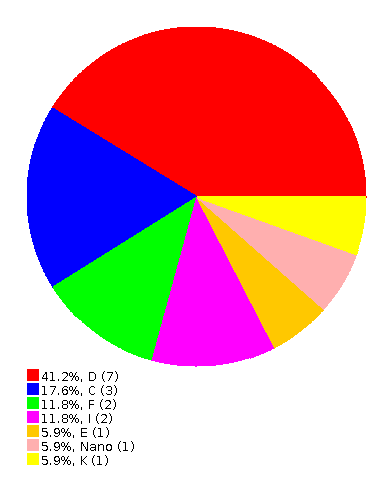
\includegraphics[scale=0.5]{../img/survey/pie.png}

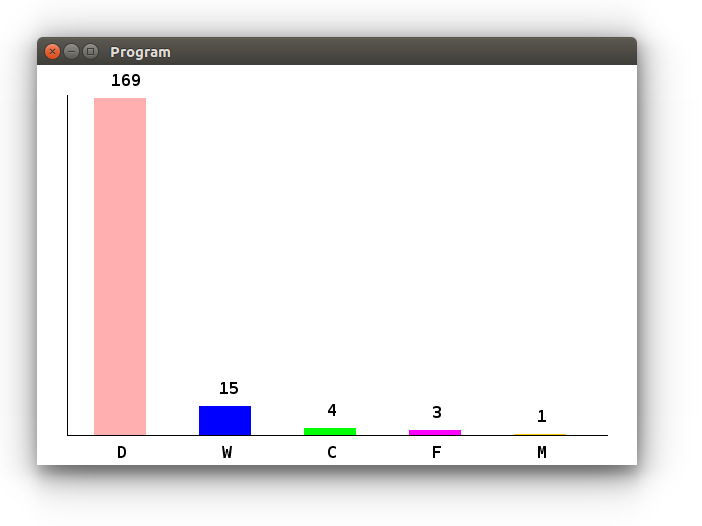
\includegraphics[scale=0.5]{../img/survey/bar.png}

%!TEX encoding = UTF-8 Unicode

%!TEX root = ../compendium2.tex

\Assignment{music}

\begin{Preparations}
\item Testa så att datorn du ska använda på redovisningen kan spela upp ljud med \code{javax.sound.midi} genom att köra igång \code{Main} i den givna koden.
\item Det är bra om du kan ta med hörlurar till datorsalen så att du inte stör andra.
\item Hämta given kod via \href{https://github.com/lunduniversity/introprog/tree/master/workspace/}{kursen github-plats} eller via hemsidan under \href{https://cs.lth.se/pgk/download/}{Download}.
\end{Preparations}

\subsection{Bakgrund}
När man skriver program skapar man ofta modeller av en viss verklig \emph{domän}, som kan vara t.ex. försäkringskassans regelverk eller en fysiksimulering i ett datorspel. För att kunna skapa sådana modeller behöver man ofta skaffa sig  \emph{domänkunskap} genom att noga sätta sig in i vad olika koncept i domänen innebär och hur de är relaterade. Med denna kunskap kan du skapa kod som modellerar domänen, utifrån noga valda förenklingar av den komplexa verkligheten. Förmåga att kunna skapa domänmodeller utgör en viktig grund för konsten att utveckla bra programvarusystem, och du kommer lära dig mer om detta i kommande kurser.

I denna laboration ska du skapa ett program baserat på en förenklad modell av domänen \emph{musik}. Du får färdig kod som modellerar hur toner är uppbyggda, samt hur olika stränginstrument fungerar.
Med denna domänmodell ska du skapa ditt eget musikprogram som använder \emph{ackord} som är uppbyggda av flera toner som spelas tillsammans.

\subsection{Domänmodell}


\subsubsection{Tonhöjd}

En \textbf{ton} \Eng{note} som spelas på ett instrument, t.ex. ett piano eller en gitarr, har en \textbf{tonhöjd} \Eng{pitch} som är relaterad till den specifika  grundfrekvens som tonens ljud har. I vår modell av musikdomänen tillordnar vi olika distinkta tonhöjder ett unikt heltal. En tonhöjd kan då beskrivas av en \code{case class Pitch(nbr: Int)} där vi använder \code{nbr} i intervallet \code{(0 to 127)}. Heltalet \code{60} motsvarar en viss ton, som även har namnet  \code{"C5"}, och som ligger ungefär i mitten av tangentbordet på ett piano.

Inom (västerländsk) musik utgår man från 12 olika \emph{tonklasser} \Eng{pitch classes}.
Dessa tolv tonklasser är ordnade i en sekvens av så kallade \emph{halva tonsteg} och har följande \textbf{tonklassnamn}:
\begin{Code}
  val pitchClassNames: Vector[String] =
    Vector("C","C#","D","D#","E","F","F#","G","G#","A","A#","B")
\end{Code}
Efter tonklassen med namnet \code{B} återkommer tonklassen med namnet \code{C}.
Symbolen \code{#} representerar en höjning ett halvt tonsteg. Tonklassen \code{C#} uttalas \emph{siss} på svenska, och \emph{see sharp} på engelska.\footnote{Man använder även b-förtecknet $\flat$, som uttalas \emph{flat} på engelska, för sänkning av en ton ett halvt tonsteg, men för enkelhetens skull bortser vi i vår modell från detta sätt att namnge toner.}
 Notera att det är ett halvt tonsteg mellan \code{E} och \code{F}, samt mellan \code{B} och \code{C} (det finns därför varken \code{E#} eller \code{B#} i listan med tonklassnamn.\footnote{Varför det är på detta viset kan du läsa mer om på t.ex. Wikipedia, men du kan också nöja dig med att det helt enkelt är så på grund av historiska skäl.})

På ett piano motsvaras de vita tangenterna av tonklassnamen \code{C D E F G A B} och de svarta tangenterna motsvaras av tonklassnamnen \code{C# D# F# G# A#}.

En s.k. \textbf{tonklass} är ett positivt heltal i intervallet \code{0 until 12} som motsvaras av index för tonklassnamnet i \code{pitchClassNames}. En tonhöjd  \code{Pitch(nbr)} tillhör tonklassen \code{nbr % 12}.

Med hjälp av heltalsdivision med 12 får man fram tonhöjdens så kallade \textbf{oktav}, alltså \code{nbr / 12}. Ett piano har normalt toner som spänner över 7 eller 8 oktaver.
En tonhöjd \code{Pitch(nbr)} kan även namnges med en kombination av tonklassnamnet och tonens oktav, t.ex. \code{"C5"}.

Med denna domänbeskrivning kan vi skapa en mer detaljerad modell av konceptet tonhöjd med hjälp av en case-klass och tillhörande kompanjonsobjekt:

\scalainputlisting[basicstyle=\ttfamily\fontsize{10}{13}\selectfont]{../workspace/w13_music_proj/src/main/scala/music/Pitch.scala}

\noindent Kompanjonsobjektet har två fabriksmetoder som kan skapa \code{Pitch}-objekt från en strängrepresentation av en tonhöjd.

\begin{itemize}[noitemsep]
  \item Metoden \code{fromString} omvandlar en sträng till en \code{Option[Pitch]}.

  \item Metoden \code {apply} kastar ett undantag om det inte går att omvandla en sträng till ett \code{Pitch}-objekt.
\end{itemize}

\Task\label{music:exceptions}\Pen Vilka två uttryck i \code{Try}-blocket kan ge undantagen \code{NumberFormatException} respektive \code{NoSuchElementException}? Undersök liknande uttryck i REPL som ger dessa undantag. Hur kan fabriksmetoden \code{fromString} skrivas om så att den använder \code{toIntOption} i stället för \code{toInt} på strängen och \code{get} i stället för \code{apply} på nyckelvärde-tabellen och utan att använda \code{scala.util.Try}? Vad finns det för nackdelar med att gå omvägen via \code{scala.util.Try} i stället för metoder som direkt ger \code{Option}?


\Task Undersök klassen \code{Pitch} i REPL.

\begin{REPL}
> sbt
sbt> console
Welcome to Scala 2.13.3 (OpenJDK 64-Bit Server VM, Java 11.0.8).
Type in expressions for evaluation. Or try :help.

scala> import music._
import music._

scala> Pitch("C#5").nbr
res0: Int = 61

scala> Pitch("C") + 1
res1: music.Pitch = Pitch("C#5")
\end{REPL}


\Subtask\Pen Ge ett exempel på argument till \code{Pitch.apply} som gör att undantag kastas.

\Subtask\Pen Ge ett exempel på argument till \code{Pitch.fromString} som ger \code{None}.

\Subtask\Pen Ge ett exempel på argument till \code{Pitch.+} som gör att undantag kastas.


\Task Ändra i implementationen av \code{fromString} så att du i stället för \code{.toOption} gör en mönstermatchning med \code{match} på \code{Try}-resultaten \code{Success} och \code{Failure} i varsin case-klausul på formen \code{case Success(x) => } och \code{case Failure(e: ???) => ???} och returnera lämpligt värde. Ta endast hand om de två förväntade undantagstyperna som du identifierade i uppgift \ref{music:exceptions}. Gör så att alla övriga eventuella undantag kastas genom denna klausul: \code{case Failure(e) => throw e}

\Subtask Testa så att din lösning fungerar i både normalfall och vid felaktigt tonhöjdsnamn.

\Subtask\Pen Undersök vad som händer om du kommenterar bort olika case-klausuler. När ger kompilatorn varning? Varför?

\Subtask\Pen Finns det någon fördel resp. nackdel med att bara fånga vissa undantag?

\subsubsection{Ackord}

Ett ackord består av flera toner som spelas tillsammans. Man kan spela ett ackord på ett stränginstrument genom att slå an en mängd toner samtidigt eller en sekvens av toner i snabb följd. Man väljer att kalla en av tonerna i ackordet (oftast den lägsta/första tonen) för \textbf{grundton} \Eng{root}.

Ett \textbf{intervall} är en tons relativa tonhöjdsavstånd från grundtonen. Ackord har olika namn beroende på vilka intervall som ingår i ackordet. Det finns väldigt många olika ackordnamn, men här begränsar vi oss för enkelhetens skull till fyra olika typer av ackord: \footnote{Om du vill veta mer om ackordnamn läs här: \url{https://en.wikipedia.org/wiki/Chord_(music)}}
\begin{itemize}
  \item dur-ackord, betecknas t.ex. \code{"C"},
  \item moll-ackord, betecknas t.ex. \code{"Cm"}
  \item sju-ackord, betecknas t.ex. \code{"C7"}
  \item maj-sju-ackord som betecknas t.ex. \code{"Cmaj7"}.
\end{itemize}

I case-klassen \code{Chord} nedan finns en metod \code{name} som definerar vilka intervall som ingår i de olika ackordtyperna ovan, utom maj-sju-ackord. Den krångliga modulo-12-omräkningen innan matchningen gör så att intervall i olika oktaver behandlas lika, även för negativa intervall.

\scalainputlisting[basicstyle=\ttfamily\fontsize{10}{13}\selectfont]{../workspace/w13_music_proj/src/main/scala/music/Chord.scala}

\Task

\Subtask Maj-sju-ackord har samma intervall som sju-ackord, förutom att det fjärde intervallet ska vara \code{11} halva tonsteg från grundtonen i stället för \code{10}. Lägg till en case-klausul i \code{Chord.name} så att maj-sju-ackord ges namn som slutar med ändelsen \code{"maj7"}.

\Subtask Testa din kod och kontrollera så att ackordet \code{Chord("D4","F#4","A4","C#5")} får namnet \code{"Dmaj7"}

\begin{REPL}
scala> Chord("D4","F#4","A4","C#5").name()
res2: String = "Dmaj7"
\end{REPL}

\Subtask Vilka fyra toner har ett \code{Cmaj7}-ackord med grundtonen \code{"C5"}?

\subsubsection{Stränginstrument}

Ett stränginstrument, t.ex. ett piano eller en gitarr, kännetecknas av att det kan spela ackord genom att flera strängar kan sättas i svängning så att många toner spelas tillsammans. I vår modell fångar vi denna egenskap med en trait \code{StringInstrument} som har en metod \code{toChordOpt} som ger något ackord om minst en sträng spelas.

Gitarr och ukulele är exempel på stränginstrument som har en greppbräda \Eng{fret board}. Man spelar på ett stränginstrument med greppbräda \Eng{fretted instrument} genom att trycka strängar mot greppbrädan med en hand, samtidigt som man knäpper på strängarna med den andra handen. Olika instanser av dessa  instrument kan skilja sig åt vad gäller antalet strängar och hur dessa strängar är stämda. En normal gitarr har 6 strängar, medan en normal ukulele bara har 4 strängar. Dessa egenskaper modelleras i koden nedan.

Varje sträng har en stämskruv med vilken kan man ändra strängens spänning,  strängens s.k. \textbf{stämning} \Eng{tuning}.  Om man knäpper på alla lösa strängarna på en gitarr med standardstämning spelas tonerna E3, A3, D4, G4, B4, E5, räknat från den tjockaste till den tunnaste strängen.

\scalainputlisting[basicstyle=\ttfamily\fontsize{10}{12.9}\selectfont]{../workspace/w13_music_proj/src/main/scala/music/instruments.scala}

Om man trycker på greppbrädans olika positioner får man olika toner, beroende på vilken position man trycker på. Positionerna på greppbrädan räknas från ett och uppåt. Position \code{0} motsvarar \textbf{lös sträng}, alltså att man slår an en sträng utan att trycka på greppbrädan över denna sträng. En negativ position, tex. \code{-1}, anger att en sträng inte spelas alls; många gitarrackord spelas genom att bara en delmängd av strängarna slås an.
Ett exempel på ett gitarrackord  visas i figur \ref{music:fig:guitar-chord}.

\Task\Pen Studera modellen av stränginstrument ovan och använd REPL för att svara på dessa frågor:

\Subtask Vad är namnet på detta pianoackord om vi väljer att lägsta tonen i ackordet är grundton: \code{Piano(Set(60, 64, 67, 70))}

\Subtask Vad heter tonerna som ingår i ackordet \code{Guitar(3,3,2,0,1,0)}.

\Subtask Vad heter detta ackord om vi väljer ett A som grundton: \code{ Ukulele(0,2,1,2)}


\begin{figure}
  \centering
  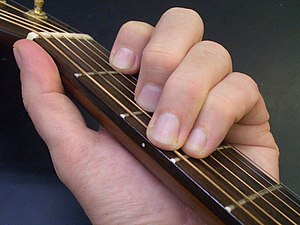
\includegraphics{../img/chords/guitar-C-major-chord.jpg}
  \caption{Ett C-dur-ackord på en gitarr motsvarande \code{Guitar(3,3,2,0,1,0)}.}
  \label{music:fig:guitar-chord}
\end{figure}


\subsubsection{Elektroniska instrument}

Ett elektroniskt instrument syntetiserar ljud med hjälp av analog och/eller digital elektronik, och kallas därför \textbf{synthesizer}, ofta förkortat \emph{synt} \Eng{synth}.

De flesta moderna PC-operativsystem inkluderar mjukvaruimplementerade syntar som följer den så kallade MIDI-standarden. Java-paketet \code{javax.sound.midi} innehåller klasser som kan få en sådan MIDI-synt att spela musik.

MIDI-standarden baseras på en modell av ett pianotangentbord där olika toner kan vara ''på'' eller ''av'' beroende på om en tangent är nedtryckt eller ej. Dessa toners höjd är modellerade på samma sätt som i vår klass \code{Pitch}, där alltså tonhöjden \code{60} motsvarar tonen \code{"C5"}, etc. En tangent kan tryckas ner olika hårt, vilket representeras av ett heltalsvärde i \code{Range(0,128)} kallat \code{velocity}. Ett högt värde ger en stark ton, medan ett litet värde motsvarar en svag (tyst) ton.

En synt som följer MIDI-standarden kan spela upp ljud via 16 olika så kallade \textbf{kanaler} \Eng{channel}, numrerade \code{(0 until 16)},  där varje kanal kan ställas in så att den spelar ett ljud som t.ex. liknar ett visst verkligt instrument, så som piano eller gitarr.

I kursens workspace i paketet \code{music} finns en \code{Synth}-modul som förenklar användningen av Java-paketet \code{javax.sound.midi}. I modulen \code{Synth} finns metoden \code{playBlocking} som kan spela flera toner under en viss tid med hjälp av synten på ditt ljudkort. Exekveringen av ditt program  blockeras tills tonerna spelats klart, därav \emph{''blocking''} i namnet.

Metoden \code{playBlocking} har följande parametrar, default-argument och returtyp:
\footnote{Om du är nyfiken kan du studera implementationen av \code{Synth}-modulen här:
\\\url{https://github.com/lunduniversity/introprog/tree/master/workspace/w13_music_proj}
 Koden blir lättare att förstå om du samtidigt läser api-dokumentationen av paketet \code{javax.sound.midi} och även lära dig mer om MIDI-standarden med hjälp av t.ex. wikipedia.}

\begin{Code}
def playBlocking(
  noteNumbers: Seq[Int] = Seq(60), // en sekvens av tonhöjder
  velocity: Int         = 60,      // hur hårt anslag i Range(0, 128)
  duration: Long        = 300,     // hur länge i millisekunder
  spread:   Long        = 50,      // millisekunder mellan tonerna
  after:    Long        = 0,       // millisekunder innan första tonen
  channel:  Int         = 0        // MIDI-kanal som spelar tonerna
): Unit
\end{Code}


\Task Anropa \code{playBlocking()} i REPL och undersök om din dator kan spela tonen \code{"C5"}. Använd gärna lurar så att du inte stör dina labbkamrater. Prova vad som händer när du ger olika argument till \code{playBlocking}.

\Task Gör klart modulen \code{ChordPlayer} enligt nedan så att metoden \code{play} kan spela ett ackord. Case-klassen \code{Strike} representerar ett ackordanslag.

\scalainputlisting[basicstyle=\ttfamily\fontsize{10}{13}\selectfont]{../workspace/w13_music_proj/src/main/scala/music/ChordPlayer.scala}

\Task Implementera ett singelobjekt med namnet \code{Test} med en \code{main}-metod som med hjälp av din \code{play}-metod från föregående uppgift spelar några olika ackord.

% \Task\Checkpoint Inför redovisningen: förbered en förklaring av koden du skrivit, med fokus på hur mönstermatchningen och undantagshanteringen fungerar.


%\clearpage

% \subsection{Frivilliga extrauppgifter}

\Task Gör en terminalapp som kan spela ackord. I kursens workspace i \code{w13_music_proj} finns en påbörjad terminalapp som du kan bygga vidare på. Den har redan en \code{Main.main}-metod som startar en loop där användaren kan ge kommando \Eng{Command Line Interface, CLI}. Kommandot \code{?} ger hjälp och kommandot \code{:q} avslutar.

\begin{REPL}
*** Welcome to music!
music> ?
?         print help
:q        quit this app
!         play chord TODO
music> !
play chord TODO
music> :q
Goodbye music!
\end{REPL}

Det finns, som syns ovan, också ett påbörjat kommando \code{!} som är tänkt att spela ett ackord, men som än så länge bara skriver ut ett TODO-meddelande. Gör så att användaren med \code{!} kan spela ackord från olika instrument enligt nedan:

\begin{REPL}
music> ! p 60 64 67
Play Piano(Set(60, 64, 67)) Chord(C5,E5,G5)
music> ! g 0 2 2 0 0 0
Play Guitar((0,2,2,0,0,0)) Chord(E3,B3,E4,G4,B4,E5)
\end{REPL}

% \noindent\emph{Tips och förslag:} Du kan i stället för \code{scala.io.StdIn.readLine} använda \code{jline} och då får du kommandohistorik med pil upp samt Ctrl+A, Ctrl+E etc. helt automatiskt. Gör helt enkelt så här i \code{Main} i stället för vanliga \code{readLine}:
% \begin{CodeSmall}
%   val console = new jline.console.ConsoleReader // skapa kommandoläsare
%   console.setExpandEvents(false) // stäng av hantering av specialtecken
%   def readLine(): String = console.readLine("music> ")
% \end{CodeSmall}
% Du behöver då lägga till jar-filen\footnote{\url{https://repo1.maven.org/maven2/jline/jline/2.14.6/jline-2.14.6.jar}} med \code{jline} till ditt bygge. Om du använder sbt kan du göra det enkelt med denna rad i filen \code{build.sbt}:
% \begin{CodeSmall}
% libraryDependencies += "jline" % "jline" % "2.14.6"
% \end{CodeSmall}
% Lägg till nedan rader i din \code{build.sbt} så att ditt program körs i en separat JVM, annars blir det konstiga initialiseringsfel av MIDI-systemet om du kör med \code{sbt run}.

% \begin{CodeSmall}
% fork                := true // https://stackoverflow.com/questions/18676712
% connectInput        := true // http://www.scala-sbt.org/1.x/docs/Forking.html
% outputStrategy      := Some(StdoutOutput)
% \end{CodeSmall}


\Task Skapa ett kommando som låter användare definierar egna namn på kommandon som sedan enkelt kan köras med hjälp av det definierade namnet. Vid definition med tidigare existerande namn så ska den gamla definitionen ersättas
\begin{REPL}
music> def Em = ! g 0 2 2 0 0 0
defined Em = ! g 0 2 2 0 0 0
music> Em
Play Guitar((0,2,2,0,0,0)) Chord(E3,B3,E4,G4,B4,E5)
\end{REPL}
Det ska fungera att föra nästlade def-kommando. Testa att definiera en hel låt som i sin tur består av definierade ackord.

\Task Du ska inför redovisningen generera automatisk dokumentation baserat på dokumentationskommentarer enligt instruktioner i Appendix \ref{appendix:doc}. Du ska skriva relevanta dokumentationskommentarer för minst hälften av dina publika metoder. Det är ofta användbart att skriva dokumentationskommentarerna \emph{före} implementationen av metodkroppen.


\subsection{Valfria uppgifter}

\Task Gör så att definitioner sparas mellan körningar.

\Task Implementera fler valfria kommandon. Du kan t.ex. 
\begin{itemize} 
\item skapa kommando som ritar en grepptabell för gitarrackord eller fingersättning på piano med \code{introprog.PixelWindow}.
\item skapa kommando för att göra drumbeats, t.ex. \code{drum mygrove x x o x} för 2 hihat + basatrumma + 1 hihat och \code{start mygrove} och \code{stop mygrove} för uppspelning av beat i bakgrunden med \code{playConcurrently}. Se i \code{Synth.scala} för vilka instrument som ger trumljud med ledning av deras namn \\\code{music.Synth.instruments.map(_.getName)}, t.ex \code{Standard Kit} eller \code{Synth Drum}. Använd kanal 10 för att spela upp trumljuden.
\end{itemize}

\Task Använd öppen-källkodsprokjektet \code{jline} i stället för \code{scala.io.StdIn.readLine} för att automatiskt få pil-upp-historik, Ctrl+A Ctrl+K etc. Se exempel på användning av \code{jline} här: \url{https://github.com/bjornregnell/termut}


% ...
%
% \vspace{7em}{\TODO OLD TEXT FROM HERE:}
%
%
% \Task ChordDraw
%
% \Subtask Rita upp en greppbräda liknande bilden nedan (kryssen läggs till i kommande uppgifter). Antalet strängar ska variera beroende på instrument.
%
% 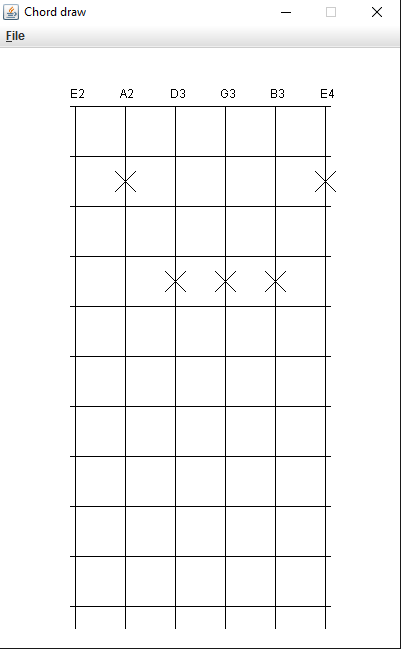
\includegraphics[width=0.5\textwidth]{../img/chords/ChordDraw}
%
% \Subtask Skapa en hjälpmetod \code{cross} som tar in två heltal $x$ och $y$. Metoden ska rita upp ett kryss som är 20x20 pixlar och har sitt centrum i den angivna koordinaten.
%
% \Subtask Rita ut ett kryss där en sträng trycks ner. \textbf{Tänk på att -1 och 0 anger att en sträng inte trycks ner}.
%
% \Subtask Implementera metoden \code{play} som börjar med att vänta på ett event från \code{SimpleWindow}, sedan kollar om eventet är av typen \code{SimpleWindow.MOUSE_EVENT}. Sedan ska man kolla om användaren tryckte på någon sträng (ett intervall på -10 till +10 i förhållande till strängens x-koordinat kan anses vara på strängen). Om användaren tryckt på en sträng ska denna spelas med hjälp av \code{SimpleNotePlayer}. Metoden \code{play} ska köras tills användaren kryssar ner fönstret, vilket motsvarar \code{SimpleWindow.CLOSE_EVENT}.
%
% \Subtask Lägg till menyvalet \code{draw} i \code{textui}. Använd \code{match} för att ta hand om felfallen att inget argument eller fler än ett argument angivits. Argumentet motsvarar ackordets plats i den filtrerade litan. Använd \code{Try} och \code{match} för att ta hand om felet att användaren anger något annat än en siffra. Använd \code{ChordDraw} för att rita upp ackord. \textbf{Kom ihåg att lägga till kommandot i listan med kommandon i \code{doCommand}}

%!TEX encoding = UTF-8 Unicode
%!TEX root = ../compendium2.tex

\Assignment{photo}

\subsection{Bakgrund}

En digital bild består av ett rutnät (en matris) av pixlar. Varje pixel har en färg, och om man har många pixlar flyter de samman för ögat så att de tillsammans skapar en bild.

Det finns olika system för hur man färgsätter de olika pixlarna. T.ex. så används CMYK-systemet (cyan, magenta, gul, svart) vid blandning av färg som ska tryckas på papper eller annat material. På en dator, däremot, används vanligtvis RGB-systemet. RGB-systemet har tre grundfärger: röd, grön och blå. Mättnaden av varje grundfärg anges av ett heltal som vi i fortsättningen förutsätter ligger i intervallet [0, 255]. 0 anger ''ingen färg'' och 255 anger ''maximal färg''. Man kan därmed representera 256 × 256 × 256 = 16 777 216 olika färgnyanser. Man kan också representera gråskalor; det gör man med färger som har samma värde på alla tre grundfärgerna: (0, 0, 0) är helt svart, (255, 255, 255) är helt vitt.

I detta projektet använder vi oss av \code{introprog.Image} för att representera en bild. Läs på om klasserna i introprog här: 
\url{https://cs.lth.se/pgk/api/}

\subsection{Uppgiften}
Du ska skriva ett program där du implementerar olika filter som ska manipulera en given bild på ett flertal olika sätt. 
Filterklasserna ska ärva från en abstrakt \code{ImageFilter}-klass.

Följande specifikation beskriver klassen \code{ImageFilter}:

\begin{ScalaSpec}{abstract class ImageFilter}
	/**
	* Create a filter object with a given name and argument descriptions.
	* @param name
	*            the name of the filter.
	* @param args
	*            optional array of strings with argument descriptions.
	*/
	abstract class ImageFilter(val name: String, val argDescriptions: String*):

		/**
		The number of args this filter needs.
		*/
		def nbrOfArgs: Int

		/**
		* Apply the filter on `img` and return the result as a new 
		* Image using the arguments in `args`.
		* 
		* @param img
		*            the original image.
		* @param args
		*            arguments
		* @return 
		*			 the resulting image.
		*/
		def apply(img: Image, args: Double*): Image

		/**
		* Calculate the intensity in each pixel of `img`.
		* 
		* @param img
		*           the image
		* @return intensitymatrix, values ranging from 0 to 255
		*/
		protected def computeIntensity(img: Image): Array[Array[Short]] = 
		   val intensity: Array[Array[Short]]

		/**
		* Convolute `p[i][j]` with the convolutionkernel `kernel`.
		* 
		* @param p
		*            matrix with numbervalues
		* @param i
		*            current row index
		* @param j
		*            current coloumn index
		* @param kernel
		*            convolutionkernel, a 3x3-matrix
		* @param weight
		*            the sum of the element in `kernel`
		* @return result of the convolution
		*/
		protected def convolve(p: Array[Array[Short]], i: Int, j: Int, 
		kernel: Array[Array[Short]], weight: Int): Short

\end{ScalaSpec}

Utöver filterklasserna ska du även skapa ett program som låter användaren välja en bild som olika filter sedan kan appliceras på.
För att åstadkomma detta ska du implementera klassen \code{ImageEditor}, som hanterar applicering av filter samt ritar bilden med hjälp av \code{PixelWindow}.



\code{ImageEditor}-klassen ska använda sig av en Stack[Image] för att hantera historiken. 
Läs dokumentationen här: \url{https://www.scala-lang.org/api/3.0.1/scala/collection/mutable/Stack.html}

\begin{ScalaSpec}{class ImageEditor}
	class ImageEditor(filters: Array[ImageFilter]):

		val history = ???

		/** 
		 * Show which filters are available and let the user choose a filter to apply. 
		 * Draw edited image in PixelWindow.
		 * User can then add more filters, undo, save image or exit.
		 *  
		 *  Example: 
		 *  0. för Blått-filter
		 *	2. för Kontrast-filter
		 * 	3. för Gauss-filter
		 *	4. för Sobel-filter
		 *	a. AVBRYT
		 *	s. SPARA
		 *	z. UNDO
		*/
		def edit(im: Image): Unit = ???

		/**Ask for arguments if required and apply filter with index `i`*/
		private def applyFilter(index: Int) = ???
\end{ScalaSpec}

Studera Scala-koden som är given här: \url{https://github.com/lunduniversity/introprog/tree/master/workspace/w13_photo}
Till din hjälp får du ett \code{ImageChooser}-objekt som hjälper dig att ladda in en bild. 
I projektet används flera klasser från kursens introprog-bibliotek. Särskilt används \code{Image, PixelWindow} och \code{IO}.
Du hittar dokumentationen till klasserna här: \url{https://cs.lth.se/pgk/api/} och du kan läsa koden här: \url{https://github.com/lunduniversity/introprog-scalalib}

\begin{ScalaSpec}{object ImageChooser}
	object ImageChooser:

		/**
		* Returns a chosen image from the images folder.
		* Prints:	
		*
		*	Välj en av följande bilder genom att mata in en siffra
		*
		*	0. boy.jpg
		*	1. car.jpg
		*	2. duck.jpg
		*	3. jay.jpg
		*	4. moon.jpg
		*	5. shuttle.jpg
		*	Ditt val: 
		*/
		def getImage: Image
\end{ScalaSpec}


\Task \textbf{Blåfilter.} Skriv en klass \code{BlueFilter} som skapar en blå version av bilden. 
Det vill säga skapa ett filter där varje pixel bara innehåller den blå komponenten. 
Testa filtret genom att skapa ett \code{Application}-object som ska innehålla en 
\code{main}-metod (\code{Application} ska användas och utökas i senare uppgifter). 
Använd \code{ImageChooser} för att välja en bild på följande sätt:
\begin{Code}
	val im = ImageChooser.getImage
\end{Code}
\begin{enumerate}
	\item Visa bilden genom att i \code{imageEditor.edit()} använda \code{pixelWindow.drawImage()}. 
	\item Alla \code{Filter}-klasser kan placeras i samma fil \code{Filters.scala}.
	\item Om du har problem med att ärva från den abstrakta \code{ImageFilter}-klassen kan du använda dig av detta exempel som endast kopierar bilden.
\end{enumerate}
\begin{ScalaSpec}{class IdentityFilter}
	class IdentityFilter(name: String) extends ImageFilter(name):
	
		def apply(im: Image, args: Double*): Image = 
			val outIm = Image.ofDim(im.width, im.height)
			outIm.update((i, j) => im(i, j))
			outIm
\end{ScalaSpec}



\Task \textbf{Inverteringsfilter.} Skriv en klass \code{InvertFilter} som inverterar en bild, dvs skapar en ''negativ'' kopia av bilden. Ljusa färger ska alltså bli mörka och mörka färger ska bli ljusa.
Fundera över vad som kan menas med en inverterad eller negativ kopia: de nya RGB-värdena är inte ett dividerat med de gamla värdena (då skulle de nya värdena kunna bli flyttal) och inte de gamla värdena med ombytt tecken (då skulle de nya värdena bli negativa).

\Task \textbf{Gråskalningsfilter.} Skriv en klass \code{GrayScaleFilter} som gör om bilden till en gråskalebild. Använd \code{ImageFilter}s \code{computeIntensity}-metod för att bestämma vilken intensitet varje pixel ska ha. Om intensiteten i en pixel till exempel är 105 så ska ett nytt \code{Color}-objekt med värdena (105, 105, 105) skapas.

\Task \textbf{Krypteringsfilter.} Skriv en klass \code{XORCryptFilter} som krypterar bilden med xor-operatorn ˆ. Denna operator gör binär xor mellan bitarna i ett heltal. Exempelvis ger 8 ˆ 127 värdet 119. Om man gör xor igen med 127, alltså 119 ˆ 127, får man tillbaka värdet 8. Varje pixel krypteras genom att använda xor-operatorn med ursprungsvärdena för rött, grönt och blått tillsammans med slumpmässiga heltalsvärden som genereras av Scalas \code{Random}-klass (tre nya slumptal för varje pixel). Låt användaren ge ett argument som seed för \code{Random}. På så sätt kan du återskapa bilden genom att applicera krypteringsfiltret igen, med samma parametervärde, på den numera krypterade bilden.

\Task \textbf{Gaussfiltrer.} Gaussfiltrering är ett exempel på så kallad faltningsfiltrering. Filtreringen bygger på att man modifierar varje bildpunkt genom att titta på punkten och omgivande punkter.

För detta utnyttjar man en så kallad faltningskärna K som är en liten kvadratisk heltalsmatris. Man placerar K över varje element i intensitetsmatrisen och multiplicerar varje element i K med motsvarande element i intensitetsmatrisen. Man summerar produkterna och dividerar summan med summan av elementen i K för att få det nya värdet på intensiteten i punkten. Divisionen med summan gör man för att de nya intensiteterna ska hamna i rätt intervall.

Exempel:

\begin{minipage}{5cm}
\begin{displaymath}
\mathit{intensity} = \left(
\begin{array}{ccccc}
5 & 4 & 2 & 8 & \ldots \\
4 & 3 & 4 & 9 & \ldots \\
9 & 8 & 7 & 7 & \ldots \\
8 & 6 & 6 & 5 & \ldots \\
\vdots & \vdots & \vdots & \vdots & \ddots
\end{array}
\right)
\end{displaymath}
\end{minipage}\hspace{2cm}
\begin{minipage}{5cm}
\begin{displaymath}
K = \left(
\begin{array}{ccc}
0 & 1 & 0 \\
1 & 4 & 1 \\
0 & 1 & 0
\end{array}
\right)
\end{displaymath}
\end{minipage}

Här är summan av elementen i $K$ $1+1+4+1+1 = 8$. För att räkna ut det nya värdet på intensiteten i punkten med index \code{(1)(1)} (det nuvarande värdet är 3) beräknar man:

\begin{displaymath}
\mathit{newintensity} = \frac{0 \cdot 5 + 1 \cdot 4 + 0 \cdot 2 + 1 \cdot 4 + 4 \cdot 3 + 1 \cdot 4 + 0 \cdot 9 + 1 \cdot 8 + 0 \cdot 7}{8} = \frac{32}{8} = 4
\end{displaymath}


Man fortsätter med att flytta K ett steg åt höger och beräknar på motsvarande sätt ett nytt värde för elementet med index \code{(1)(2)} (där det nuvarande värdet är 4 och det nya värdet blir 5). Därefter gör man på samma sätt för alla element utom för ”ramen” dvs elementen i matrisens ytterkanter.

Skriv en klass \code{GaussFilter} som implementerar denna algoritm. Varje färg ska behandlas separat. Gör på följande sätt:
\begin{enumerate}
	\item Bilda tre \code{short}-matriser och lagra pixlarnas red-, green- och blue-komponenter i matriserna.
	\item Utför faltningen av de tre komponenterna för varje element och updatera outIm med de uträknade värdena.
	\item Elementen i ramen behandlas inte, men i \code{outIm} måste också dessa element få värden. Enklast är att flytta över dessa element oförändrade från \code{im} till \code{outIm}. Man kan också sätta dem till \code{Color.WHITE}, men då kommer den filtrerade bilden att se något mindre ut.
\end{enumerate}

Använd \code{ImageFilter}s \code{convolve}-metod för att utföra faltningen. Metoden behöver en faltningsmatris, \code{kernel}, som input och ska anropas med red-, green- och blue-matrisen. Faltningsmatrisen kan vara ett attribut i klassen och ska ha följande utseende:

\begin{displaymath}
\begin{pmatrix}
  0 & 1 & 0 \\
  1 & 4 & 1 \\
  0 & 1 & 0 \\
\end{pmatrix}
\end{displaymath}

Det kan vara intressant att prova med andra värden än 4 i mitten av faltningsmatrisen. Med värdet 0 får man en större utjämning eftersom man då inte alls tar hänsyn till den aktuella pixelns värde. Låt användaren mata in argument för mittvärdet via terminalen.

Anmärkning: det kan ibland vara svårt att se någon skillnad mellan den filtrerade bilden och originalbilden. Om man vill ha en riktigt suddig bild så måste man använda en större matris som faltningskärna.


\Task  \textbf{Sobelfiltrer.} Sobelfiltrering är, precis som Gaussfiltrering, en typ av faltningsfiltrering. Med Sobelfiltrering får man dock motsatt effekt i jämförelse med Gaussfiltrering, dvs man förstärker konturer i en bild. I princip deriverar man bilden i x- och y-led och sammanställer resultatet.

\begin{figure}[H]
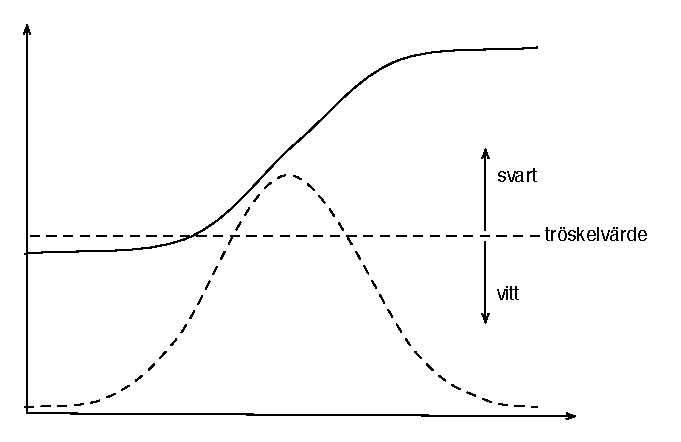
\includegraphics[width=0.9\textwidth]{../img/w12-assignment-photo/derivatabild2.pdf}
\caption { En funktion (heldragen linje) och dess derivata (streckad linje).}
\label{fig:photo:sobelfilter:derivatabild}
\end{figure}

I figur~\ref{fig:photo:sobelfilter:derivatabild} visas en funktion $f$ (heldragen linje) och funktionens derivata $f'$ (streckad linje). Vi ser att där funktionen gör ett ''hopp'' så får derivatan ett stort värde. Om funktionen representerar intensiteten hos pixlarna längs en linje i x-led eller y-led så motsvarar ''hoppen'' en kontur i bilden. Om man sedan bestämmer sig för att pixlar där derivatans värde överstiger ett visst tröskelvärde ska vara svarta och andra pixlar vita så får man en bild med bara konturer.

Nu är ju intensiteten hos pixlarna inte en kontinuerlig funktion som man kan derivera enligt vanliga matematiska regler. Men man kan approximera derivatan, till exempel med följande formel:

\begin{displaymath}
f'(x) \approx \frac{f(x+h) - f(x-h)}{2h}
\end{displaymath}

(Om man här låter $h$ gå mot noll så får man definitionen av derivatan.) Uttryckt i Scala och matrisen \code{intensity} så får man:

\begin{Code}
val derivative = (intensity(i)(j+1) - intensity(i)(j-1)) / 2
\end{Code}

Allt detta kan man uttrycka med hjälp av faltning.

\begin{enumerate}
	\item Beräkna intensitetsmatrisen med metoden \code{computeIntensity}.
	\item Falta varje punkt i intensitetsmatrisen med två kärnor:
$$
X\_SOBEL =
\begin{pmatrix}
  -1 & 0 & 1 \\
  -2 & 0 & 2 \\
  -1 & 0 & 1 \\
\end{pmatrix}
Y\_SOBEL =
\begin{pmatrix}
  -1 & -2 & -1 \\
  0 & 0 & 0 \\
  1 & 2 & 1 \\
\end{pmatrix}
$$
	Använd metoden \code{convolve} med vikten 1. Koefficienterna i matrisen $X\_SOBEL$ uttrycker derivering i x-led, i $Y\_SOBEL$ faltning i y-led. För att förklara varför koefficienterna ibland är 1 och ibland 2 måste man studera den bakomliggande teorin noggrant, men det gör vi inte här.
	\item Om resultaten av faltningen i en punkt betecknas med \code{sx} och \code{sy} så får man en indikator på närvaron av en kontur med \code{math.abs(sx) + math.abs(sy)}. Absolutbelopp behöver man eftersom man har negativa koefficienter i faltningsmatriserna.
	\item  Sätt pixeln till svart om indikatorn är större än tröskelvärdet, till vit annars. Låt tröskelvärdet bestämmas av ett argument som användaren kan ange.
\end{enumerate}

Skriv en klass \code{SobelFilter} som implementerar denna algoritm.

\begin{figure}[H]
\begin{center}
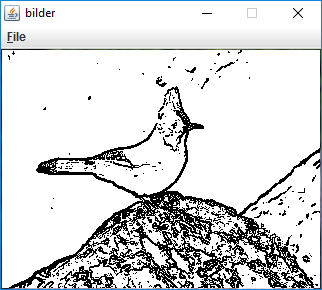
\includegraphics[width=0.6\textwidth]{../img/w12-assignment-photo/sobeljay.png}
\caption { Exempel på en bild där ett Sobelfilter applicerats med ett parametervärde på 150.}
\label{fig:photo:sobelfilter:sobel}
\end{center}
\end{figure}


\Task Implementera \code{ImageEditor} enligt specifikationerna ovan.

\Task Knyt ihop allt i \code{Application}-objektet som du skapade innan. Utskrifterna ska se ut på följande sätt:\newline

{\setlength{\parindent}{0cm}

 Välj en av följande bilder genom att mata in en siffra\newline

0. boy.jpg\newline
1. car.jpg\newline
2. duck.jpg\newline
3. jay.jpg\newline
4. moon.jpg\newline
5. shuttle.jpg\newline
Ditt val: \textbf{1}\newline
Bild car.jpg laddad\newline
\textit{//Bilden visas i ett PixelWindow}\newline

Välj ett alternativ\newline

0. för Blåfilter\newline
1. för Inverterat\newline
2. för Krypterat\newline
3. för Inverterat\newline
4. för Grått\newline
5. för Kontrast\newline
6. för Gauss\newline
7. för Sobel\newline
8. för Intervall\newline
9. för Change\newline
a. AVBRYT\newline
s. SPARA\newline
z. UNDO\newline

Ditt val: \textbf{6}\newline
Till detta filter behöver du ange [1] argument.\newline

Ange argument för Gauss: \newline
Argument 1: [Styrka (0-50) där 0 är max]: \textbf{0}\newline
\textit{//Bilden uppdateras och ritas i samma PixelWindow}\newline

Välj ett alternativ\newline
...
}

Tänk på att användaren kan mata in otillåtna värden. Detta ska hanteras på lämpligt sätt.

\subsection{Frivilliga extrauppgifter}

\Task \textbf{Kontrastfilter.} Om man applicerar kontrastfiltrering på en färgbild så kommer bilden att konverteras till en gråskalebild (Man kan naturligtvis förbättra kontrasten i en färgbild och få en färgbild som resultat. Då behandlar man de tre färgkanalerna var för sig). Många bilder lider av alltför låg kontrast. Det beror på att bilden inte utnyttjar hela det tillgängliga området 0–255 för intensiteten. Man får en bild med bättre kontrast om man ''töjer ut'' intervallet enligt följande formel (linjär interpolation):

\begin{Code}
val newIntensity = 255 * (intensity - 45) / (225 - 45)
\end{Code}

Som synes kommer en punkt med intensiteten 45 att få den nya intensiteten 0 och en punkt med intensiteten 225 att få den nya intensiteten 255. Mellanliggande punkter sprids ut jämnt över intervallet \code{[0, 255]}. För punkter med en intensitet mindre än 45 sätter man den nya intensiteten till 0, för punkter med en intensitet större än 225 sätter man den nya intensiteten till 255. Vi kallar intervallet där de flesta pixlarna finns för \code{[lowCut, highCut]}. De punkter som har intensitet mindre än \code{lowCut} sätter man till 0, de som har intensitet större än \code{highCut} sätter man till 255. För de övriga punkterna interpolerar man med formeln ovan (45 ersätts med \code{lowCut}, 225 med \code{highCut}).

Det återstår nu att hitta lämpliga värden på \code{lowCut} och \code{highCut}. Detta är inte något som kan göras helt automatiskt, eftersom värdena beror på intensitetsfördelningen hos bildpunkterna. Man börjar med att beräkna bildens intensitetshistogram, dvs hur många punkter i bilden som har intensiteten 0, hur många som har intensiteten 1, . . . , till och med 255.

I de flesta bildbehandlingsprogram kan man sedan titta på histogrammet och interaktivt bestämma värdena på \code{lowCut} och \code{highCut}. Så ska vi dock inte göra här. I stället bestämmer vi oss för ett procenttal \code{cutOff}, som användaren kan ange som argument från terminalen, och som  beräknar \code{lowCut} så att \code{cutOff} procent av punkterna i bilden har en intensitet som är mindre än \code{lowCut} och \code{highCut} så att \code{cutOff} procent av punkterna har en intensitet som är större än \code{highCut}.

Exempel: antag att en bild innehåller 100 000 pixlar och att \code{cutOff} är 1.5. Beräkna bildens intensitetshistogram i en array
\begin{Code}
val histogram = Array[Int](256)
\end{Code}

Beräkna \code{lowCut} så att \code{histogram(0)} + \ldots + \code{histogram(lowCut)} = 0.015 * 100000 (så nära det går att komma, det blir troligen inte exakt likhet). Beräkna \code{highCut} på liknande sätt.

Sammanfattning av algoritmen:
\begin{enumerate}
	\item Beräkna intensiteten hos alla punkterna i bilden, lagra dem i en \code{short}-matris. Använd den färdigskrivna metoden \code{computeIntensity}.
	\item Beräkna bildens intensitetshistogram.
	\item Argument från användaren användas som \code{cutOff}.
	\item Beräkna \code{lowCut} och \code{highCut} enligt ovan.
	\item Beräkna den nya intensiteten för varje pixel enligt interpolationsformeln och lagra de nya pixlarna i \code{outIm}.
\end{enumerate}
Skriv en klass \code{ContrastFilter} som implementerar algoritmen. I katalogen \emph{images} kan bilden \emph{moon.jpg} vara lämplig att testa, eftersom den har låg kontrast. Anmärkning: om \code{cutOff} sätts = 0 så får man samma resultat av denna filtrering som man får av \code{GrayScaleFilter}. Detta kan man se genom att studera interpolationsformeln.

\Task \textbf{Eget filter.} Skapa ett eget filter som utnyttjar att \code{apply}-metoden tar emot en sekvens av värden. Till exempel så kan du skicka in en array med fem värden där de två första värdena representerar ett intesitetsintervall och de tre sista värdena representerar röd-, grön- och blåkomponenterna till en färg som ska stoppas in där intensiteten hamnar utanför det givna intervallet. Ett annat alternativ kan vara att använda sig av metoder i \code{PixelWindow} för att välja specifika pixlar på originalbilden som sedan kan användas för att manipulera bilden i filtrets \code{apply}-metod. Valet är ditt!


%\renewcommand{\section}{\chapter}
%\renewcommand{\subsection}{\section}
%%!TEX encoding = UTF-8 Unicode
\chapter{Muntlig examen}\label{chapter:W14}


\end{document}
